\chapter{Empirical Results and Evaluation}
\label{ch:empirical_results_evaluation}

This chapter presents empirical results from executing the demonstration scenarios defined in Section \ref{sec:prototype_scenarios}.
The evaluation compares development workflow performance across native, containerized, and virtualized environments, examining both toolchain switching efficiency and comprehensive build performance.
All quantitative measurements followed the statistical methodology outlined in Section \ref{sec:methodology_evaluation}, with 30 repetitions per operation to ensure statistical robustness.
Two-tailed independent samples t-tests validated the statistical significance of observed performance differences, with complete results documented in Appendix~\nameref{appendix:statistical_tests}.

\section{Scenario 1: Toolchain switching performance}

This scenario evaluates the time required to switch between different development toolchains, addressing the practical challenge of developers needing to work with multiple compiler versions or validate cross-distribution compatibility.
The scenario measures the overhead associated with changing the development environment configuration across the three deployment approaches.
Where direct comparisons were possible (Docker Desktop vs native Linux containers), statistical testing confirmed significant performance differences for image pull operations ($p < 0.001$) and container start times ($p = 0.031$); detailed results are available in Appendix~\nameref{appendix:statistical_tests}.

\subsection{Overview of toolchain switching results}

Before examining the detailed breakdown of each environment, Figure~\ref{fig:scenario1_wall_time_overview} presents a comparative overview of wall-clock times across all measured operations.

\begin{figure}[htbp]
    \centering
    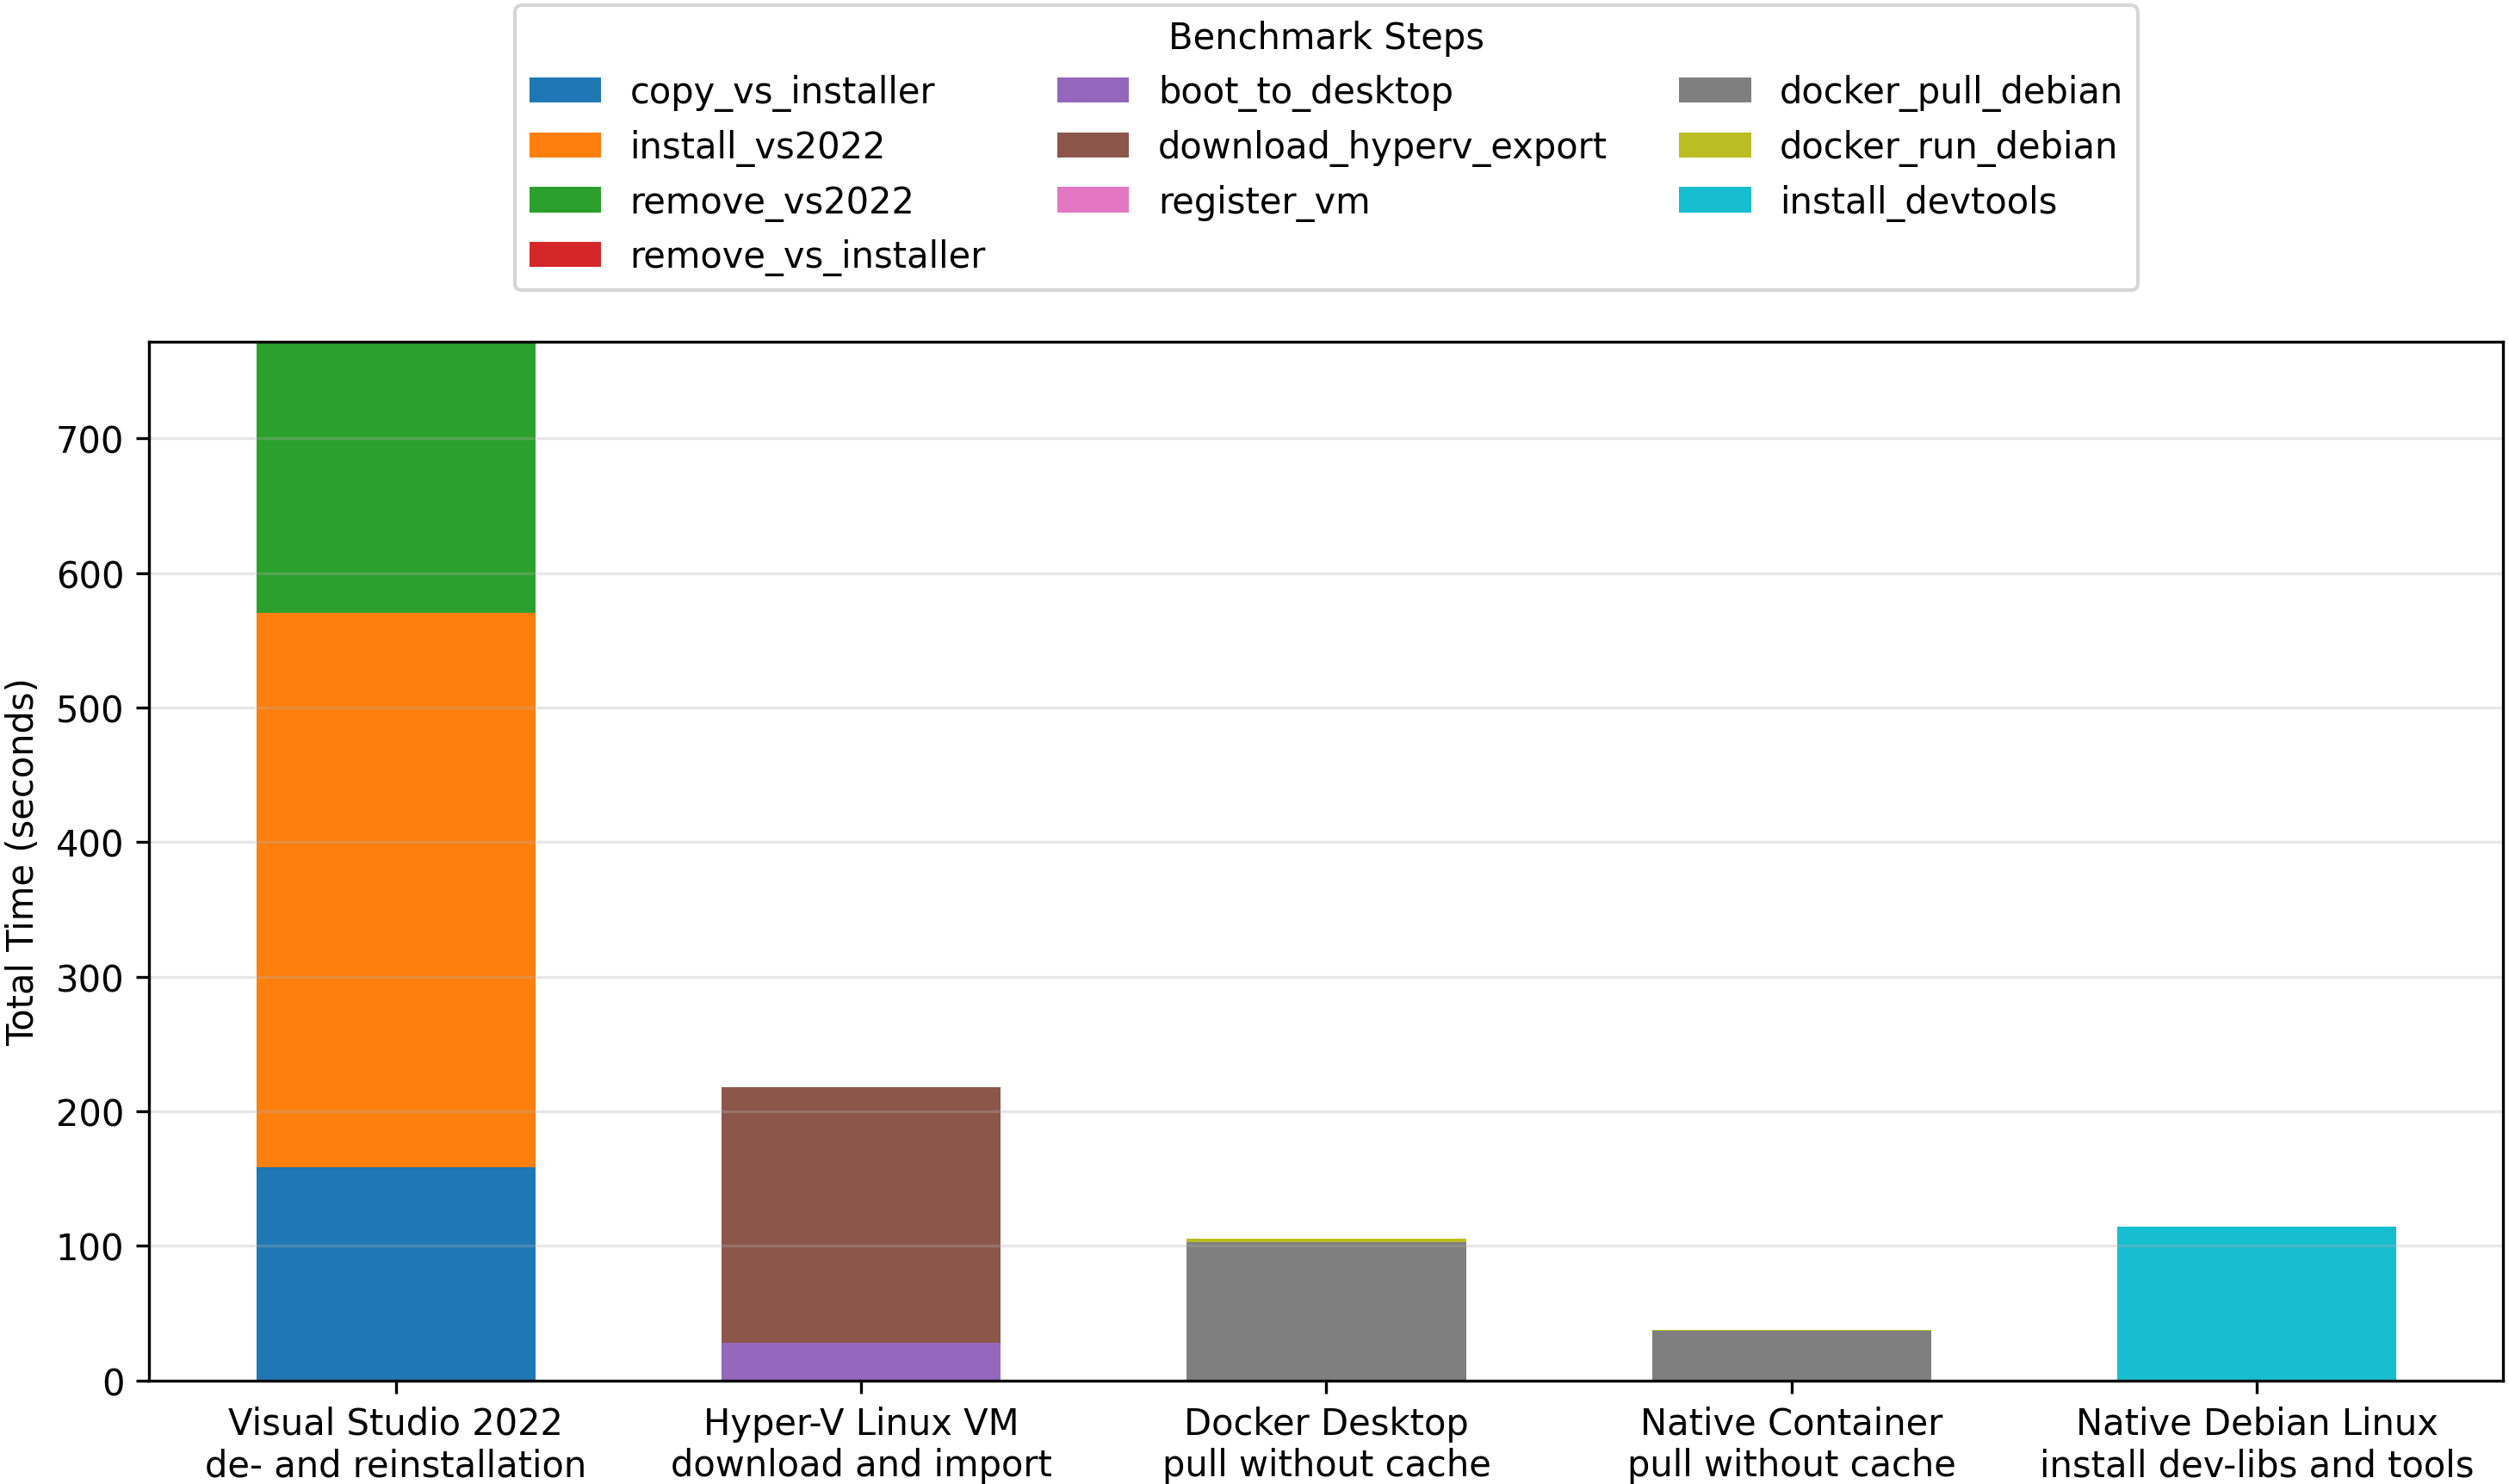
\includegraphics[width=\linewidth]{figures/scenario_1_wall_time.png}
    \caption{Wall time comparison (mean) across all toolchain switching operations (n=30)}
    \label{fig:scenario1_wall_time_overview}
\end{figure}

The figure, based on mean values, shows a clear performance hierarchy: native Windows toolchain switching via Visual Studio de- and reinstallation requires approximately 12.9 minutes, while containerized approaches complete in under 2 minutes---native containers on Linux at 37.5 seconds and Docker Desktop on Windows at approximately 1.7 minutes.
The Hyper-V virtualized approach falls between these at approximately 3.6 minutes.
Following subsections examine each environment's performance characteristics in detail, with a comprehensive statistical comparison presented in Section \ref{subsec:toolchain_switching_comparison}.

\subsection{Native Windows: Visual Studio toolchain switching}

This test measures the time required to switch between Visual Studio 2022 Latest and Visual Studio 2022 LTS versions on native Windows installations.
The process involves complete uninstallation of the existing version followed by installation of the target version, representing the traditional approach to toolchain management.

\begin{table}[htbp]
    \centering
    \begin{tabular}{|l|c|c|c|c|c|}
        \hline
        \textbf{Operation} & \textbf{Mean (s)} & \textbf{Median (s)} & \textbf{Std Dev} & \textbf{Min (s)} & \textbf{Max (s)} \\
        \hline
        VS2022 Uninstall & 201.02 & 201.10 & 4.91 & 189.72 & 210.52 \\
        Installer Removal & 0.44 & 0.44 & 0.10 & 0.29 & 0.65 \\
        Installer Copy & 158.45 & 158.62 & 1.61 & 155.15 & 160.92 \\
        VS2022 Install & 411.84 & 413.07 & 6.58 & 398.90 & 422.22 \\
        \hline
        \textbf{Total} & \textbf{771.75} & \textbf{772.25} & \textbf{8.77} & \textbf{758.69} & \textbf{789.92} \\
        \hline
    \end{tabular}
    \caption{Visual Studio 2022 toolchain switching breakdown (n=30)}
    \label{tab:native_vs_breakdown}
\end{table}

\begin{figure}[htbp]
    \centering
    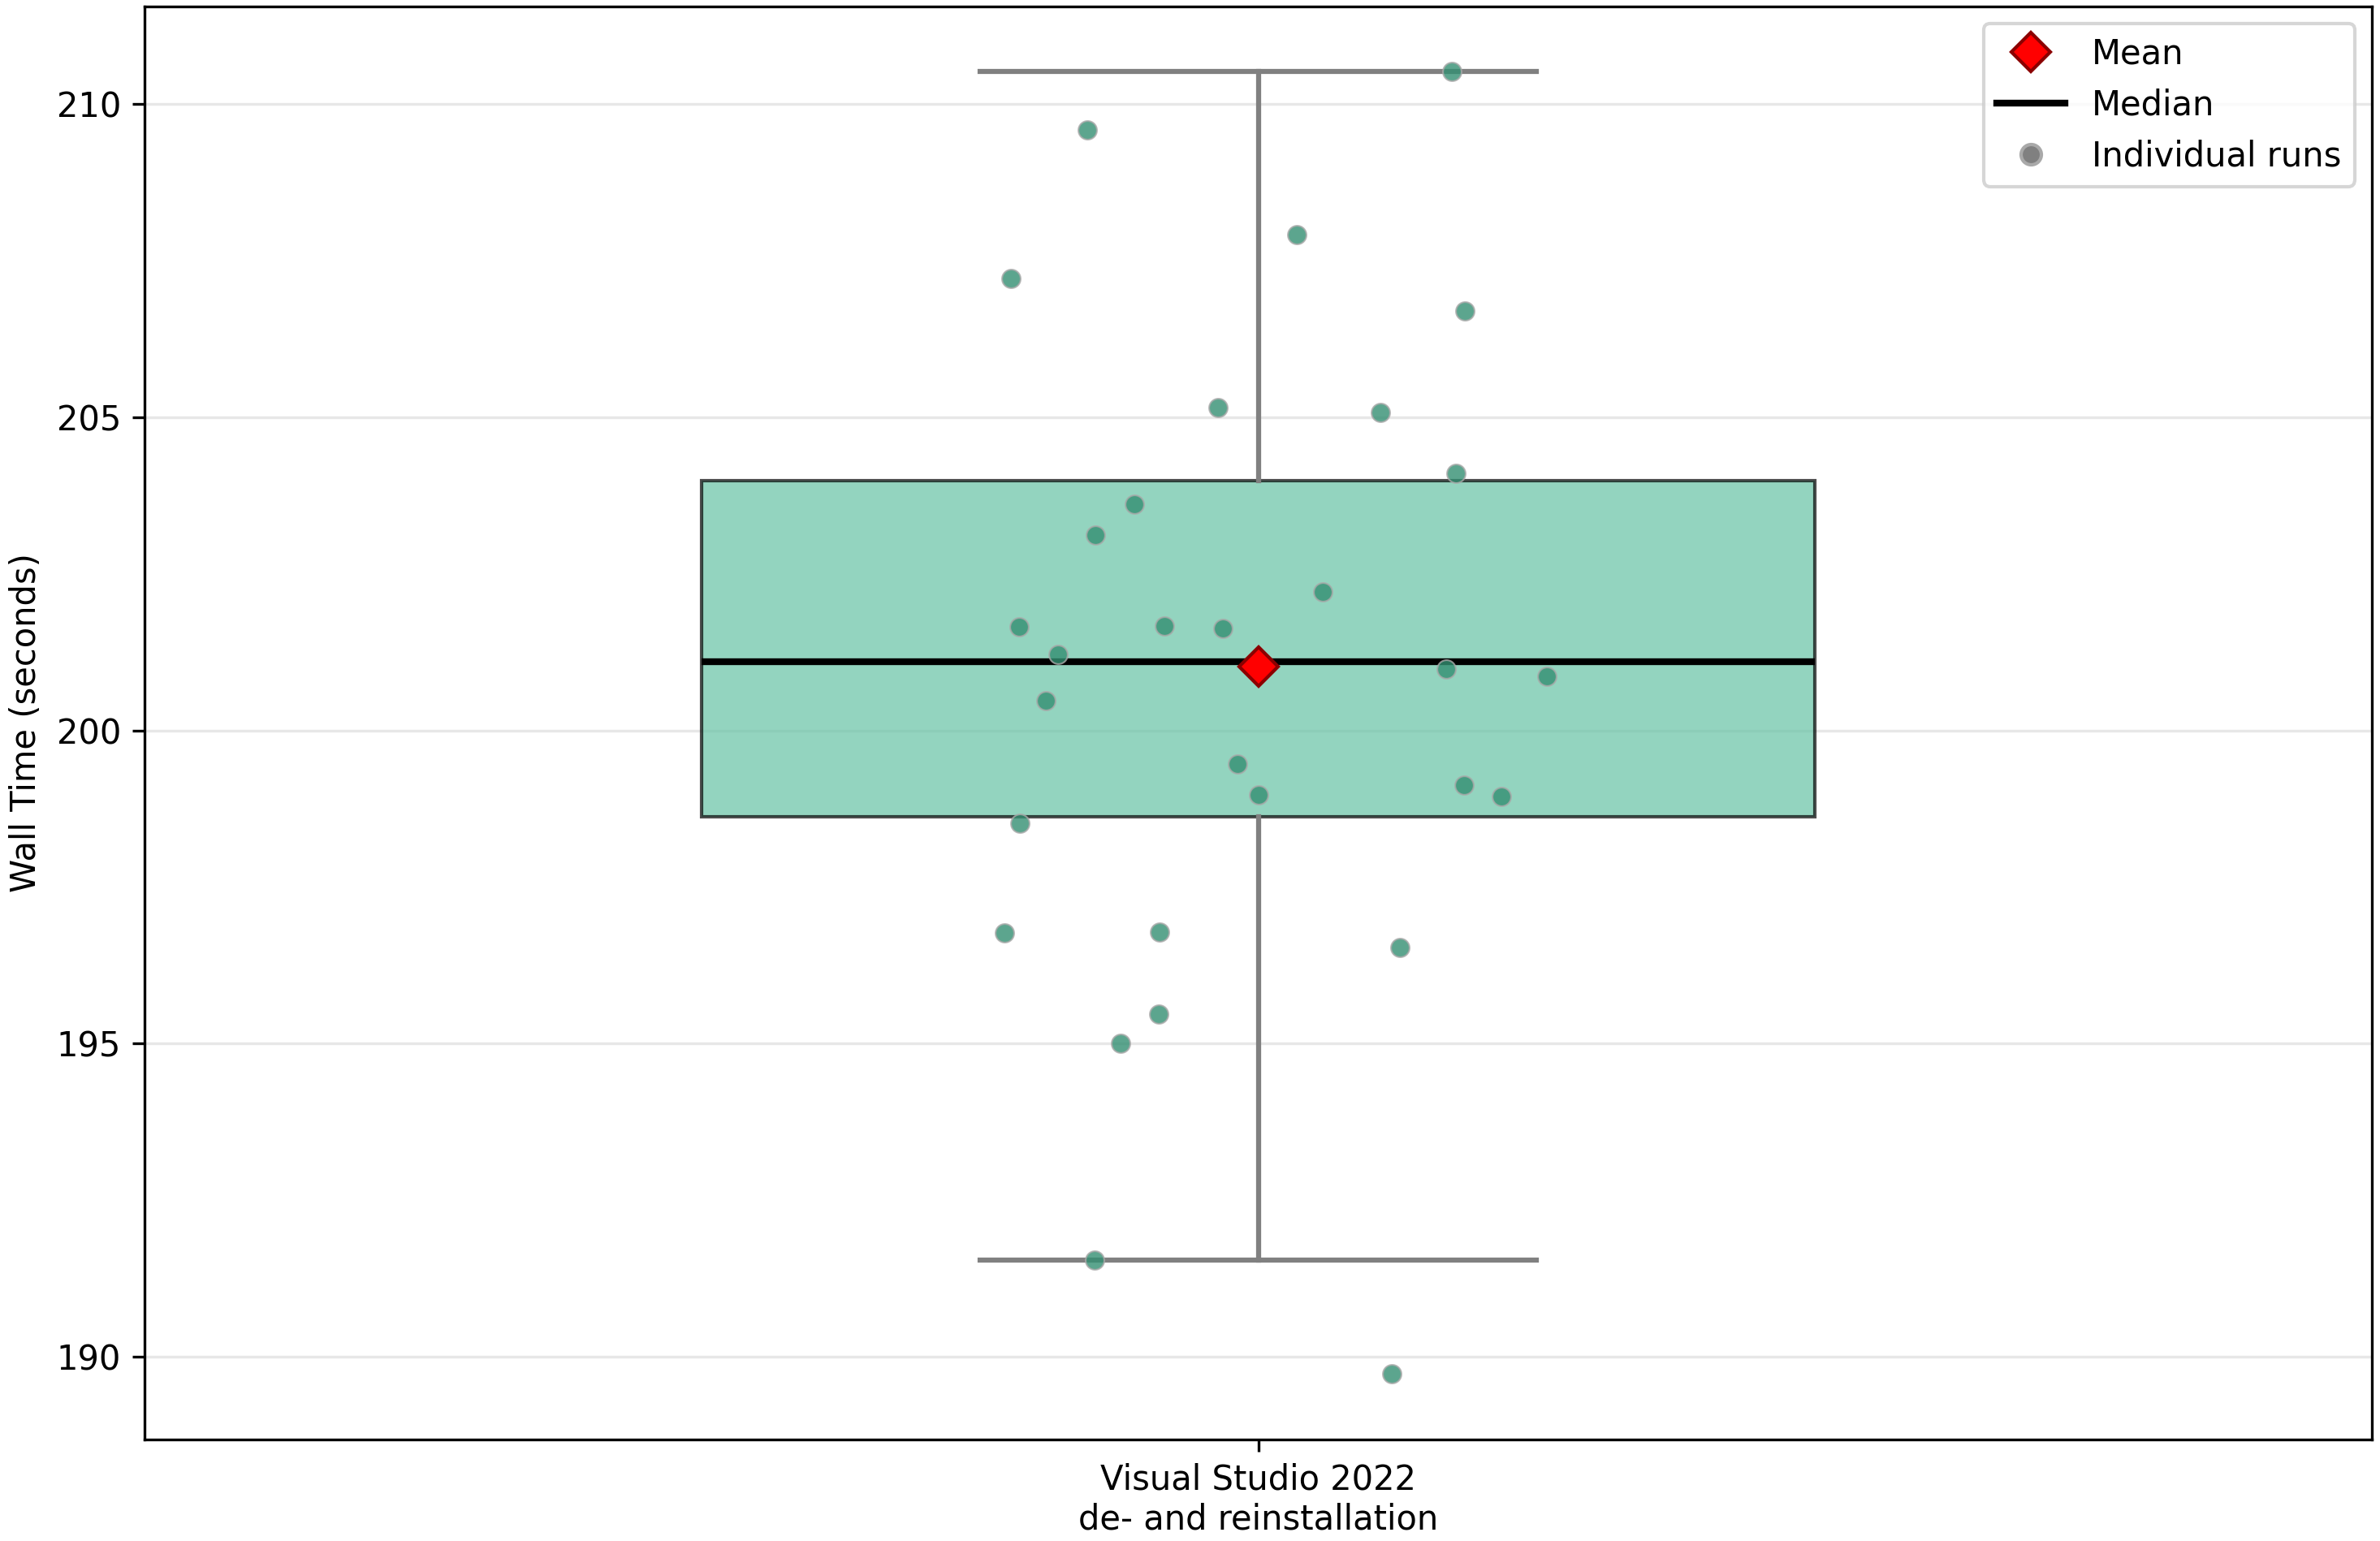
\includegraphics[width=0.8\linewidth]{figures/scenario_1_boxplot_remove_vs2022_wall_time.png}
    \caption{Visual Studio 2022 uninstallation time distribution (n=30)}
    \label{fig:native_vs_uninstall}
\end{figure}

\begin{figure}[htbp]
    \centering
    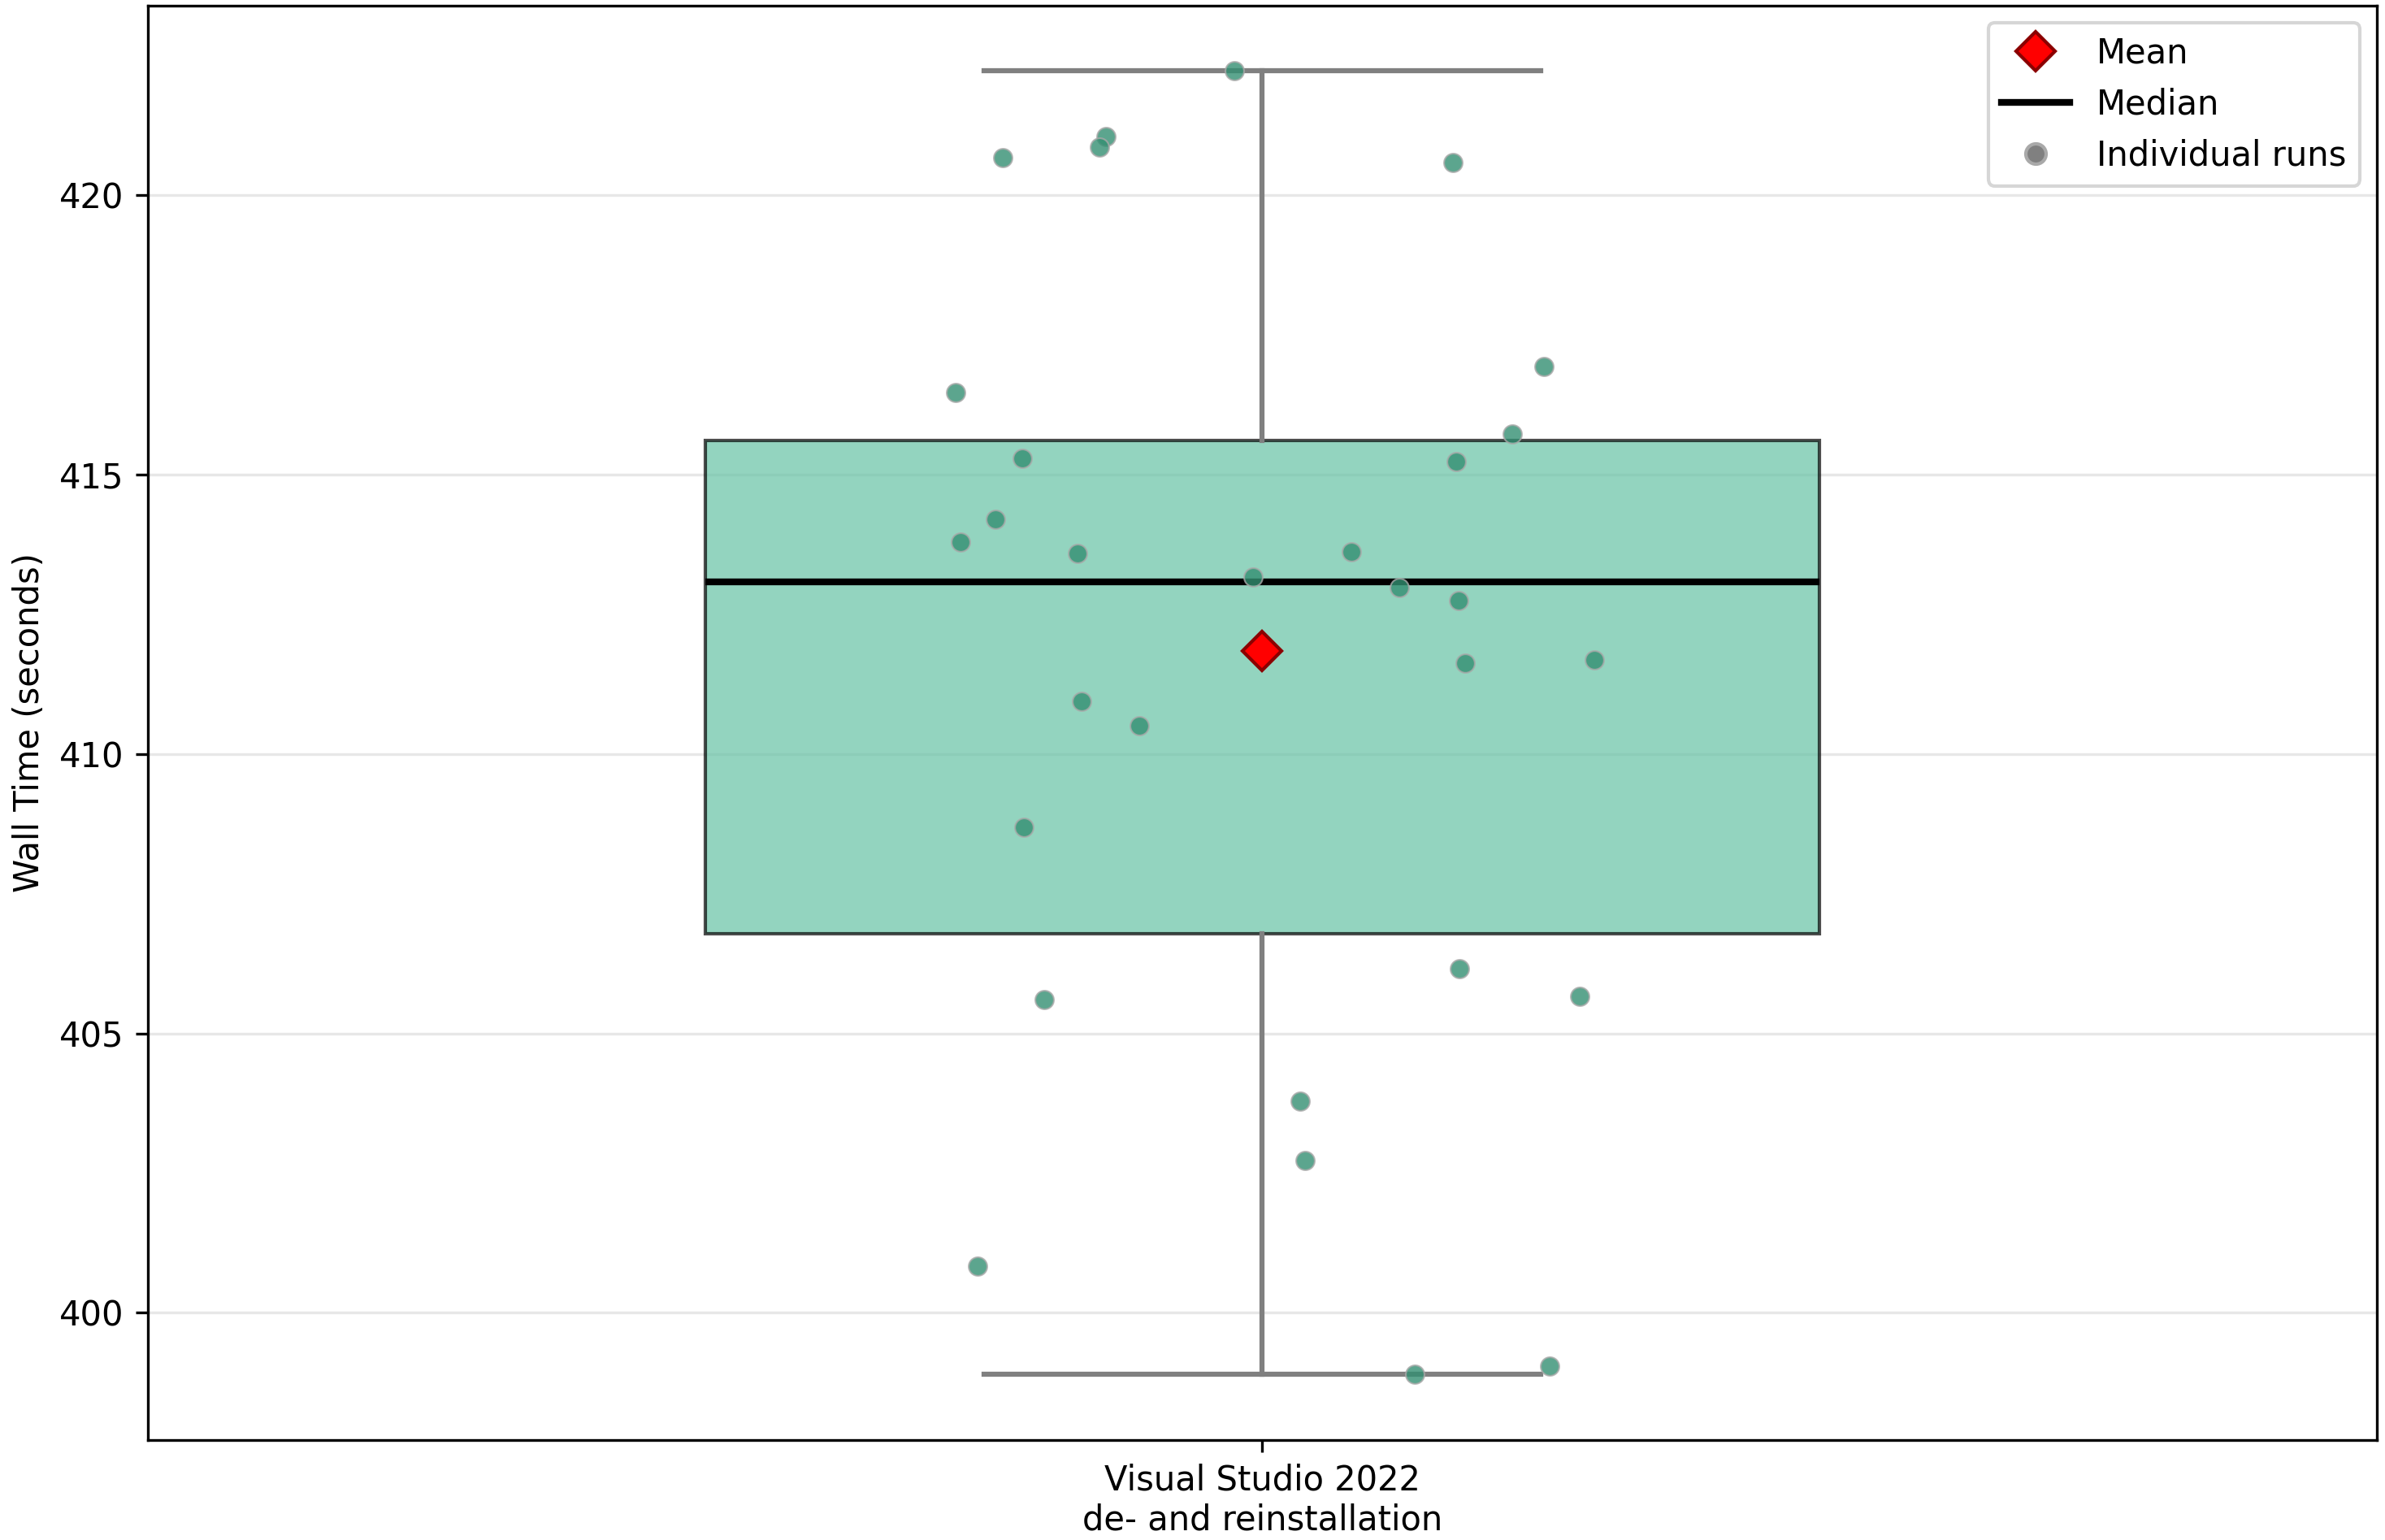
\includegraphics[width=0.8\linewidth]{figures/scenario_1_boxplot_install_vs2022_wall_time.png}
    \caption{Visual Studio 2022 installation time distribution (n=30)}
    \label{fig:native_vs_install}
\end{figure}

The complete native Windows toolchain switch requires approximately 12.9 minutes, with installation accounting for 53\% of the total time, uninstallation for 26\%, installer copying for 21\%, and installer removal for less than 0.1\%.
The Visual Studio uninstallation process shows consistent timing (standard deviation of 4.91 seconds), indicating primarily I/O-bound operations involving systematic removal of components, registry entries, and cached data.
The installer removal step (0.44 seconds) is negligible, representing cleanup of the previous Visual Studio installer executable.
Installation dominates the switching process at approximately 6.9 minutes, encompassing package extraction, component configuration, SDK installation, and system integration.

\subsection{Containerized: Image switching}

This test measures the time required to switch between Debian 12 container images, representing the containerized approach to toolchain management.
Two container runtime configurations were evaluated: Docker Desktop on Windows (with WSL2 backend) and native Docker Engine on Linux.

\begin{table}[htbp]
    \centering
    \begin{tabular}{|l|l|c|c|c|c|c|}
        \hline
        \textbf{Operation} & \textbf{Environment} & \textbf{Mean (s)} & \textbf{Median (s)} & \textbf{Std Dev} & \textbf{Min (s)} & \textbf{Max (s)} \\
        \hline
        \multirow{2}{*}{Image Pull} & Docker Desktop & 102.66 & 98.93 & 8.02 & 92.61 & 123.01 \\
        & Native Container & 36.52 & 36.53 & 0.04 & 36.43 & 36.59 \\
        \hline
        \multirow{2}{*}{Container Start} & Docker Desktop & 2.34 & 0.55 & 3.43 & 0.41 & 12.21 \\
        & Native Container & 0.95 & 0.95 & 0.04 & 0.89 & 1.10 \\
        \hline
        \multirow{2}{*}{\textbf{Total}} & \textbf{Docker Desktop} & \textbf{105.00} & \textbf{100.78} & \textbf{10.02} & \textbf{93.02} & \textbf{126.50} \\
        & \textbf{Native Container} & \textbf{37.48} & \textbf{37.48} & \textbf{0.05} & \textbf{37.34} & \textbf{37.60} \\
        \hline
    \end{tabular}
    \caption{Container toolchain switching breakdown (n=30)}
    \label{tab:container_breakdown}
\end{table}

\begin{figure}[htbp]
    \centering
    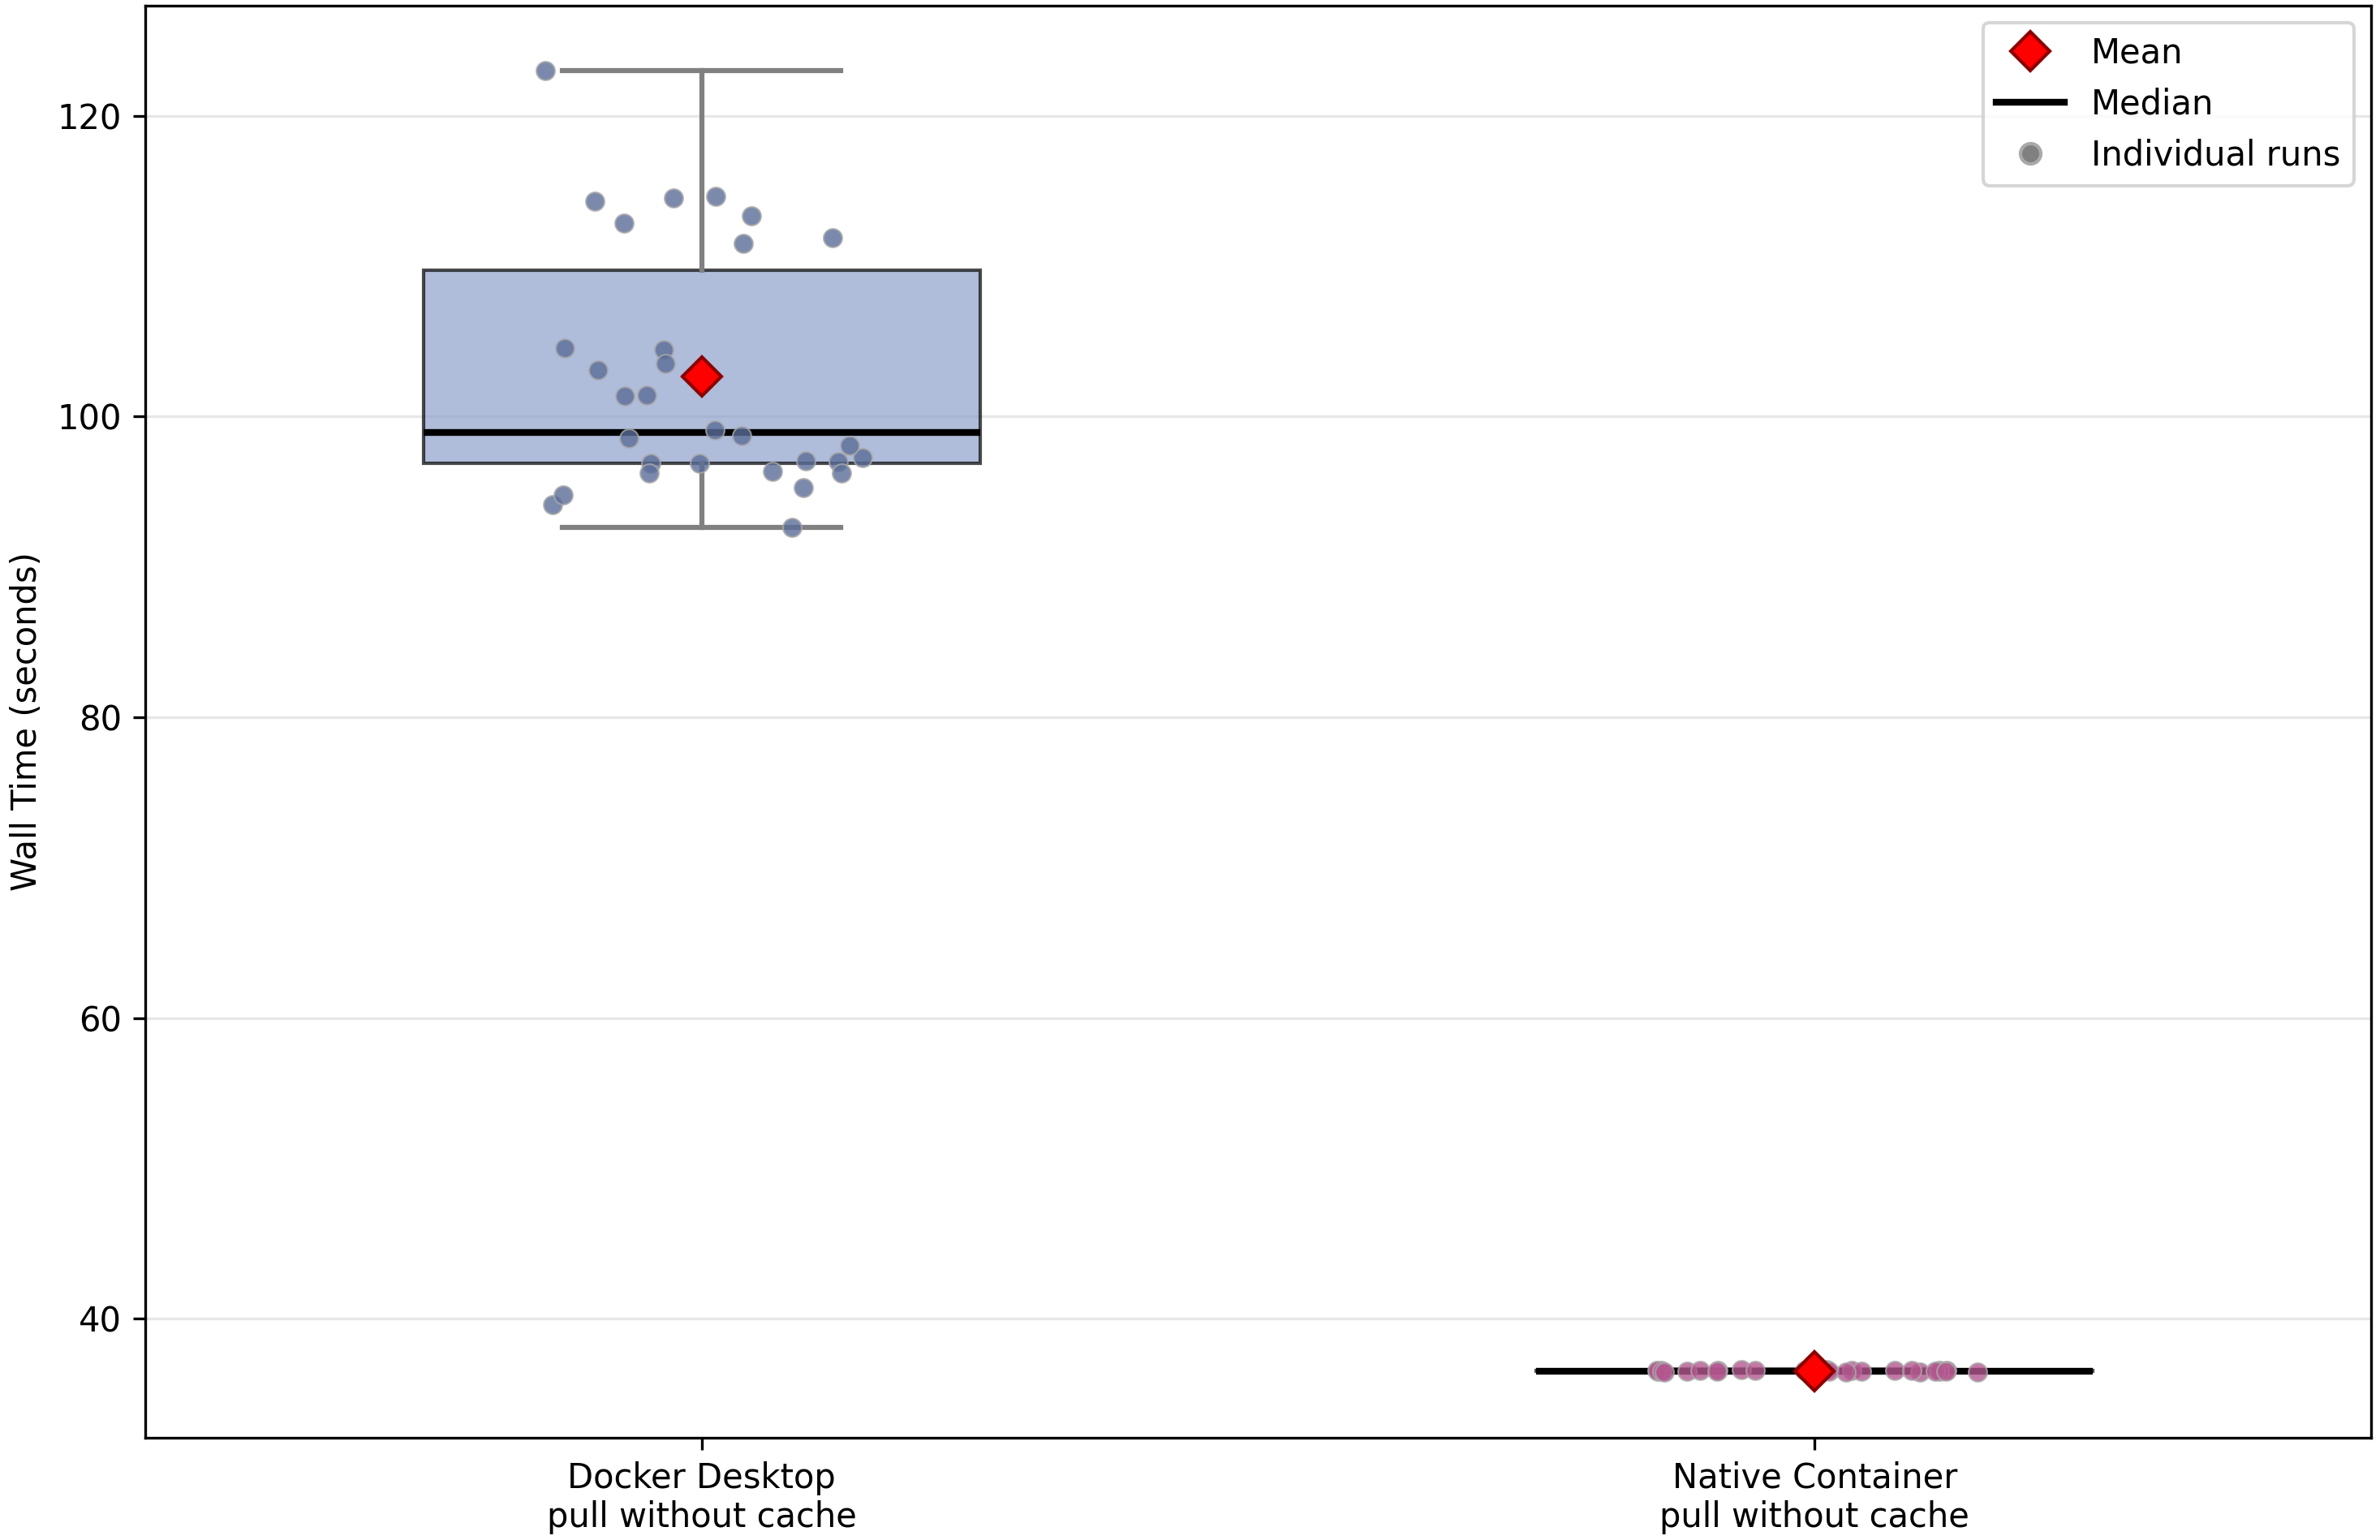
\includegraphics[width=0.8\linewidth]{figures/scenario_1_boxplot_docker_pull_debian_wall_time.png}
    \caption{Container image pull time distribution (n=30)}
    \label{fig:container_image_pull}
\end{figure}

\begin{figure}[htbp]
    \centering
    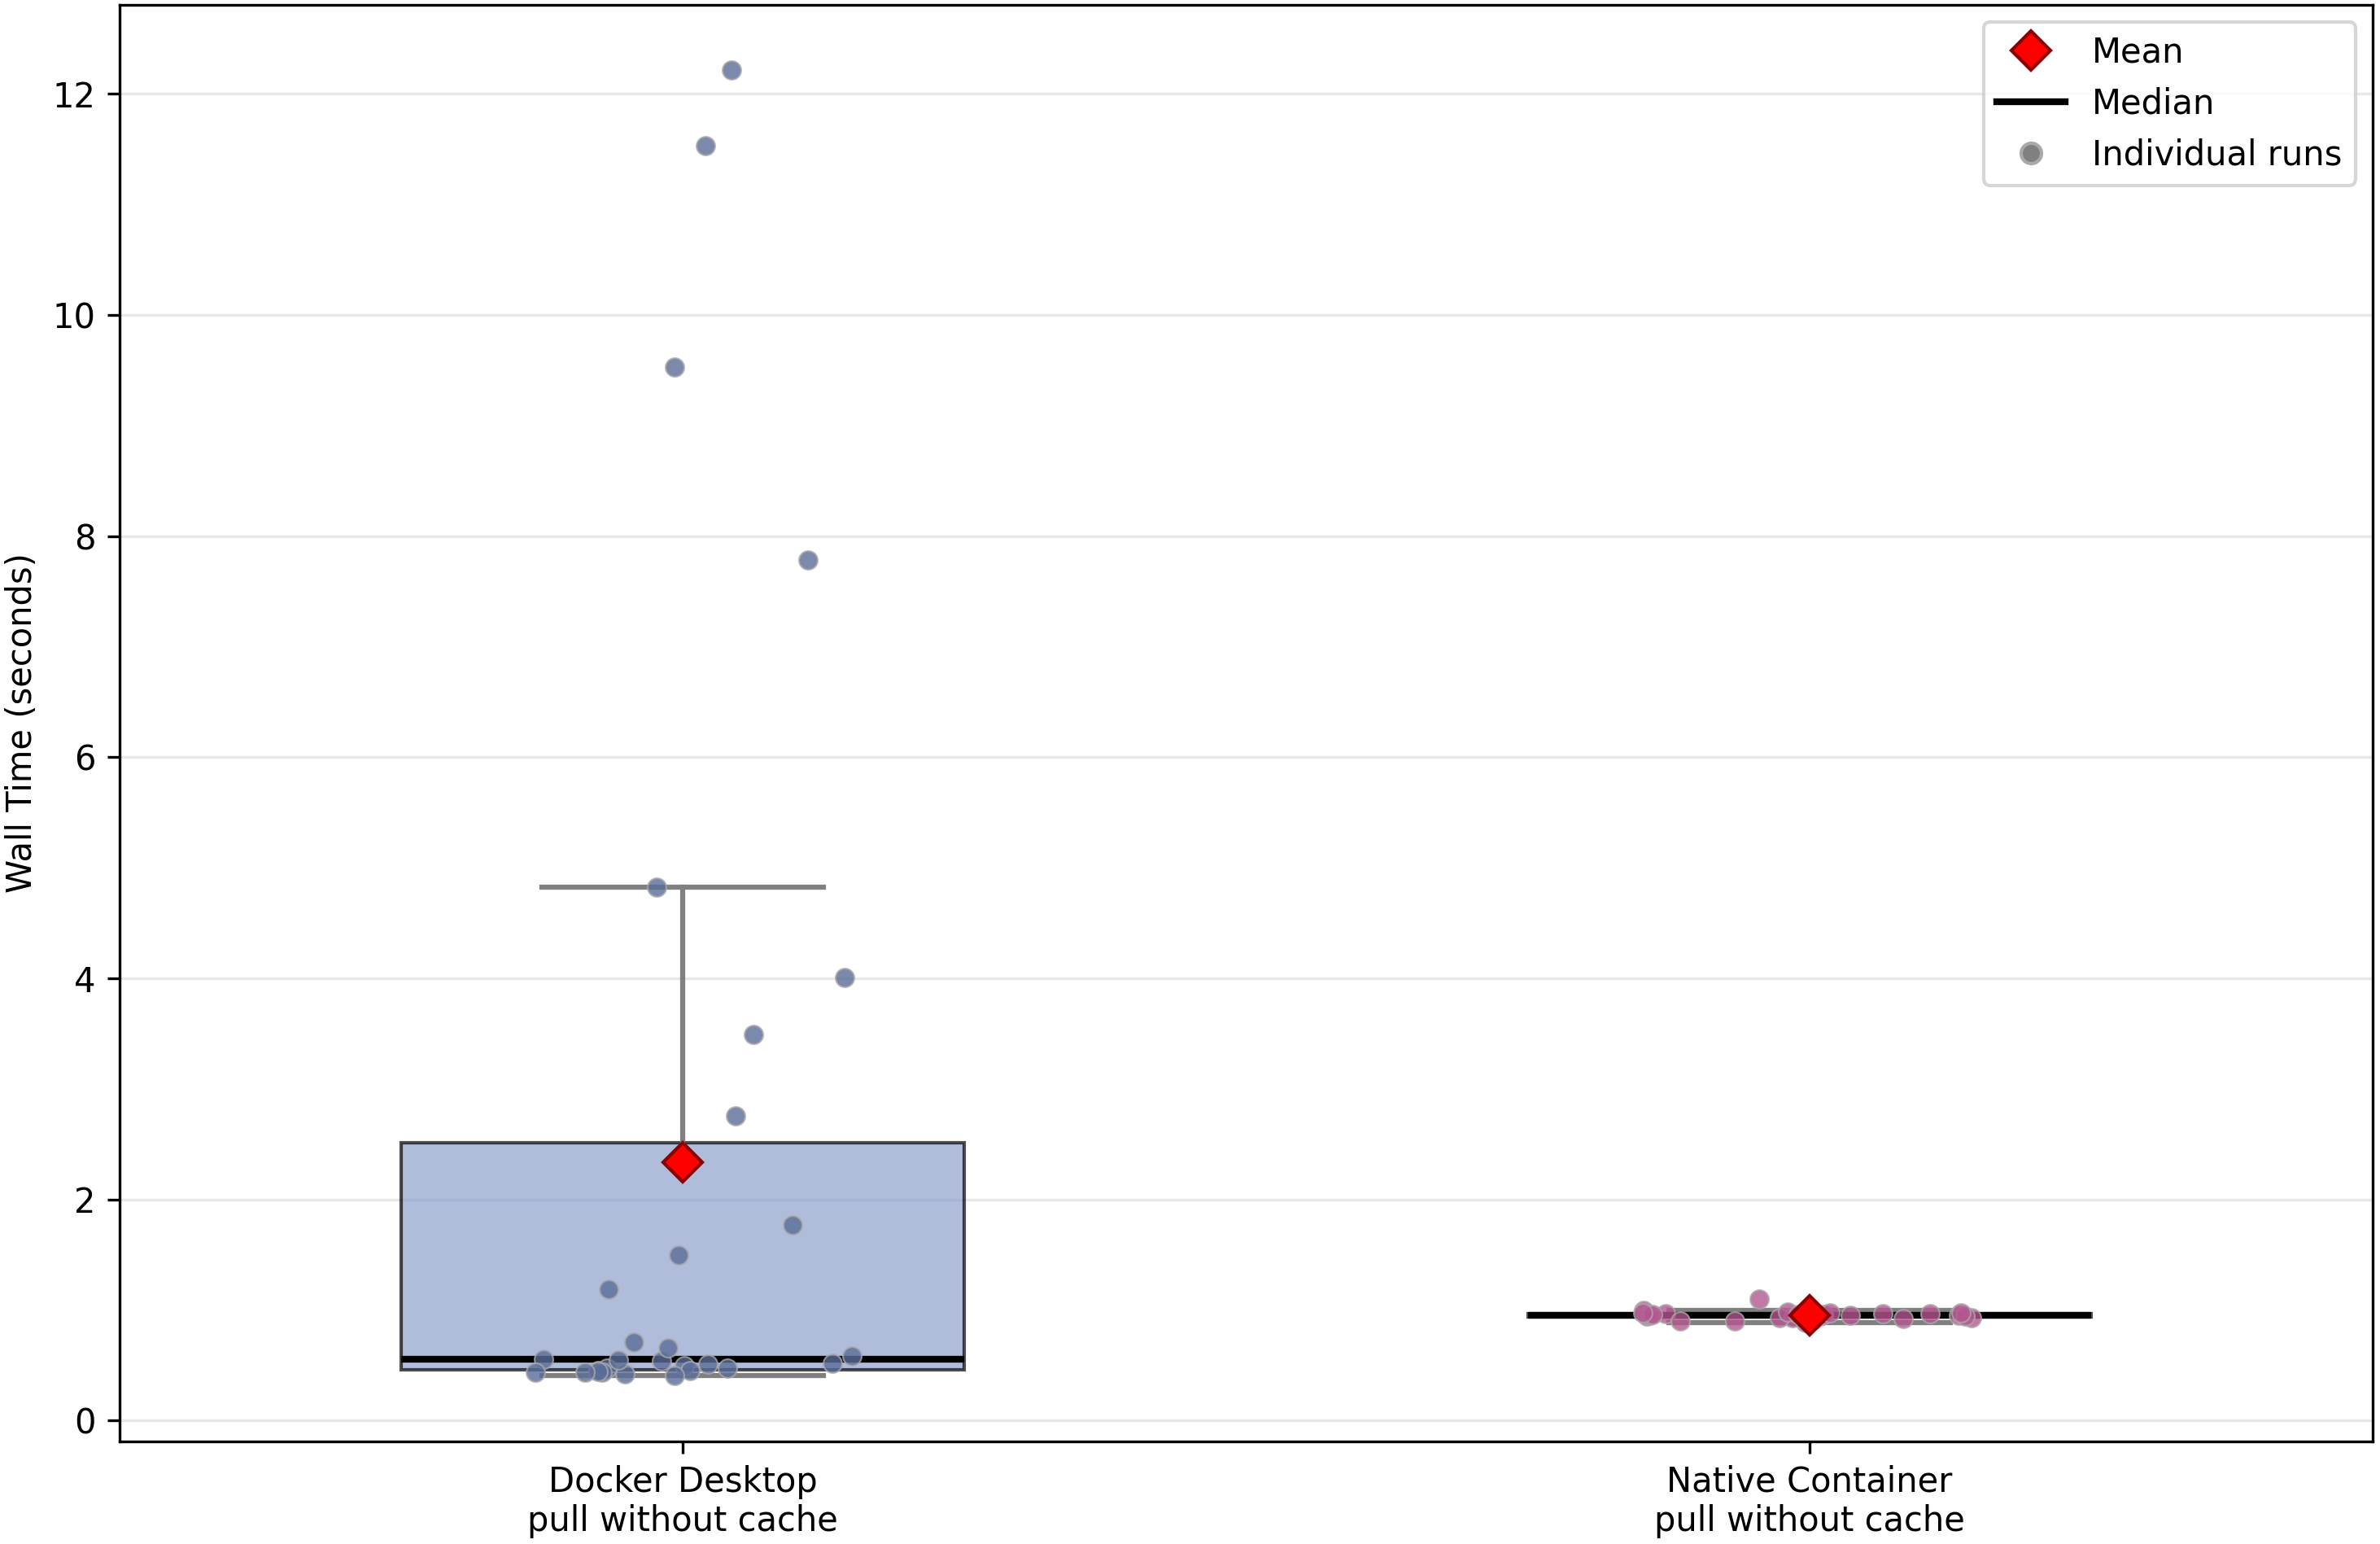
\includegraphics[width=0.8\linewidth]{figures/scenario_1_boxplot_docker_run_debian_wall_time.png}
    \caption{Container start time distribution (n=30)}
    \label{fig:container_start}
\end{figure}

Native Linux containers complete the image pull in 36.5 seconds with high consistency (standard deviation of 0.04 seconds), while Docker Desktop requires 98.9 seconds.

Container startup contributes minimally to total switching time (2--3\% across both environments).
Docker Desktop's median start time of 0.55 seconds indicates most runs complete quickly, but occasional outliers (maximum 12.21 seconds) reflect WSL2 VM initialization overhead when resuming from idle state.

Total containerized toolchain switching achieves 37.5 seconds on native Linux and 100.8 seconds (1.68 minutes) on Docker Desktop, representing 95.1\% and 87.0\% improvements over the native Windows baseline respectively.

\subsection{Virtualized: Hyper-V VM template switching}

This test measures the time required to switch to a Hyper-V virtual machine template, representing the virtualized approach to toolchain management where complete operating system environments are managed as VMs.

\begin{table}[htbp]
    \centering
    \begin{tabular}{|l|c|c|c|c|c|}
        \hline
        \textbf{Operation} & \textbf{Mean (s)} & \textbf{Median (s)} & \textbf{Std Dev} & \textbf{Min (s)} & \textbf{Max (s)} \\
        \hline
        Template Download & 189.67 & 188.75 & 10.02 & 173.38 & 214.22 \\
        VM Registration & 0.51 & 0.52 & 0.06 & 0.44 & 0.70 \\
        VM Boot & 28.00 & 28.00 & 1.91 & 25.00 & 32.00 \\
        \hline
        \textbf{Total} & \textbf{218.18} & \textbf{217.48} & \textbf{9.99} & \textbf{200.53} & \textbf{242.73} \\
        \hline
    \end{tabular}
    \caption{VM toolchain switching breakdown (n=30)}
    \label{tab:vm_breakdown}
\end{table}

\begin{figure}[htbp]
    \centering
    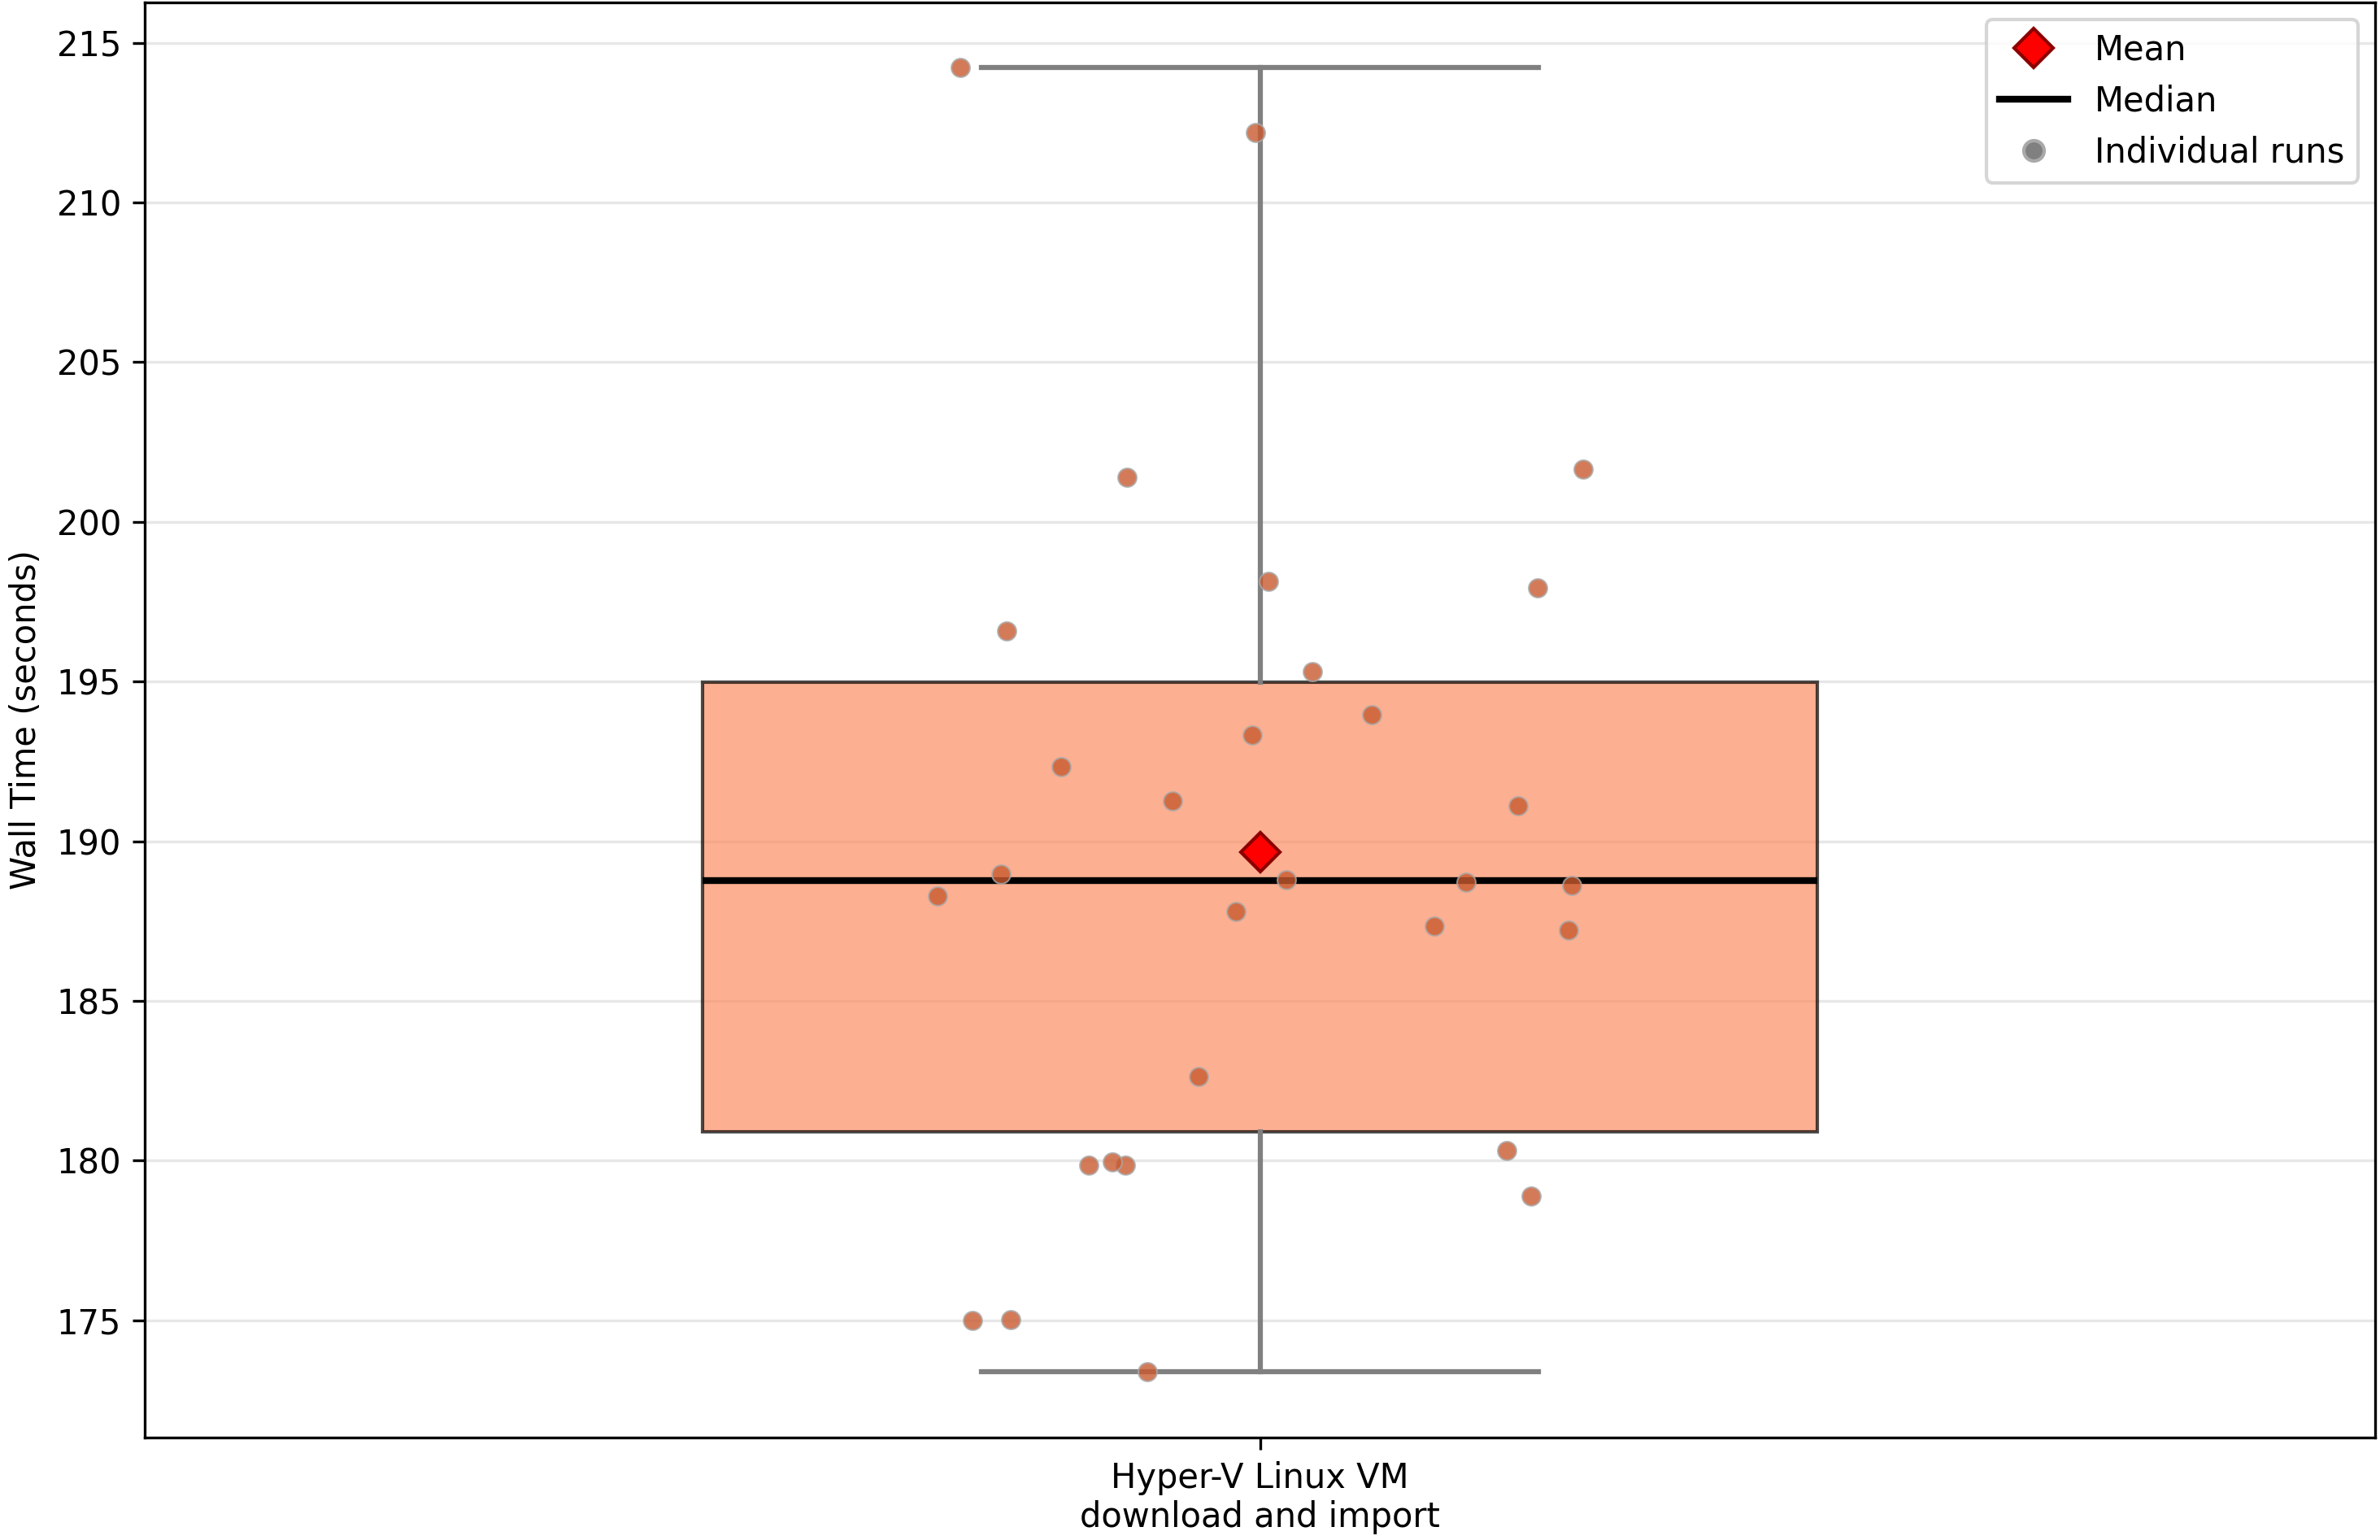
\includegraphics[width=0.8\linewidth]{figures/scenario_1_boxplot_download_hyperv_export_wall_time.png}
    \caption{VM template download time distribution (n=30)}
    \label{fig:vm_template_download}
\end{figure}

\begin{figure}[htbp]
    \centering
    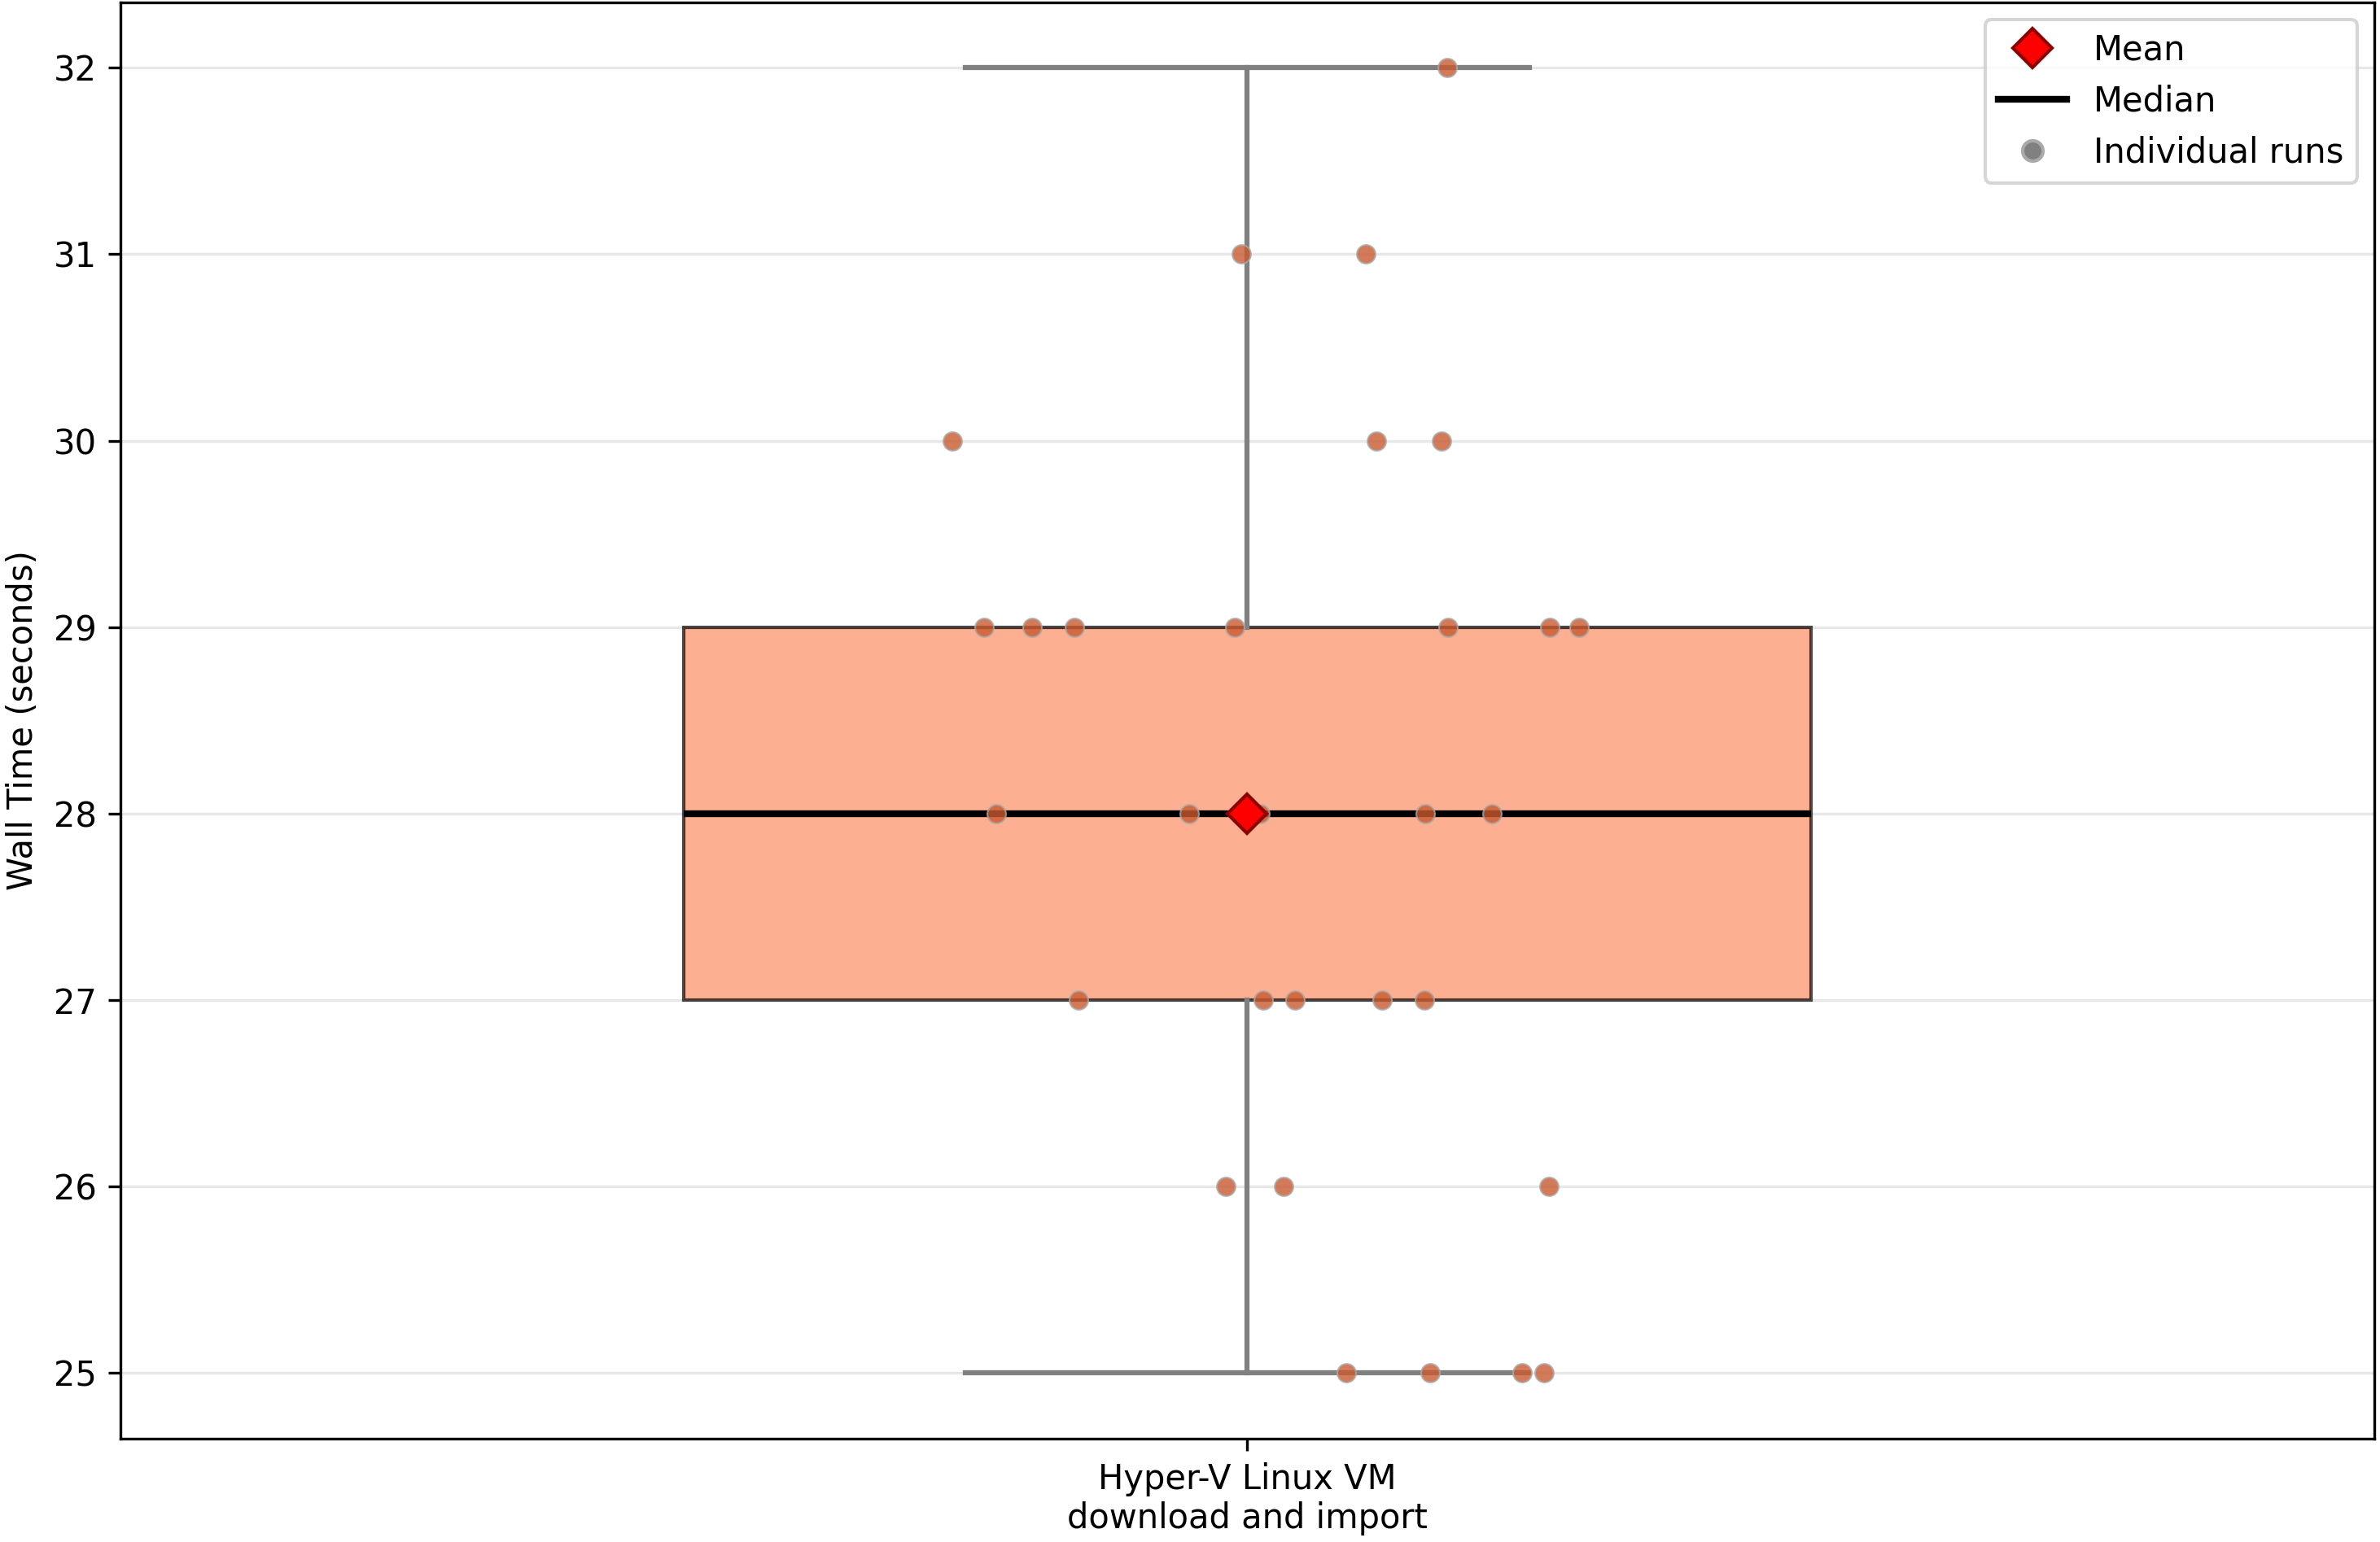
\includegraphics[width=0.8\linewidth]{figures/scenario_1_boxplot_boot_to_desktop_wall_time.png}
    \caption{VM boot time distribution (n=30)}
    \label{fig:vm_boot}
\end{figure}

The total virtualized toolchain switching time of 217.5 seconds (3.6 minutes) is dominated by the template download operation (87\%), with VM boot contributing 13\% and registration being negligible.
VM template download requires approximately 3.1 minutes, with moderate variance reflecting network bandwidth fluctuations during transfer of large VHDX files over a 1GbE connection.
These measurements used a Linux VM template of 20.5 GB; VM template size significantly impacts the total switching time.
VM registration is nearly instantaneous at 0.52 seconds, as Hyper-V efficiently handles configuration metadata operations.
VM boot requires approximately 28 seconds for full operating system initialization with consistent performance across runs.

This represents a 71.7\% improvement over the native Windows baseline, positioning virtualization between native installation and containerization in terms of switching efficiency.

\subsection{Native Linux: Development tools installation}

For completeness, the benchmark also measured the time to install development tools on a native Debian Linux system, representing the traditional Linux development environment setup approach.

\begin{table}[htbp]
    \centering
    \begin{tabular}{|l|c|}
        \hline
        \textbf{Metric} & \textbf{Value (seconds)} \\
        \hline
        Mean & 114.47 \\
        Median & 109.00 \\
        Std.\ Deviation & 22.99 \\
        Min & 90.00 \\
        Max & 174.00 \\
        \hline
    \end{tabular}
    \caption{Native Linux development tools installation time (n=30)}
    \label{tab:native_linux_devtools}
\end{table}

\begin{figure}[htbp]
    \centering
    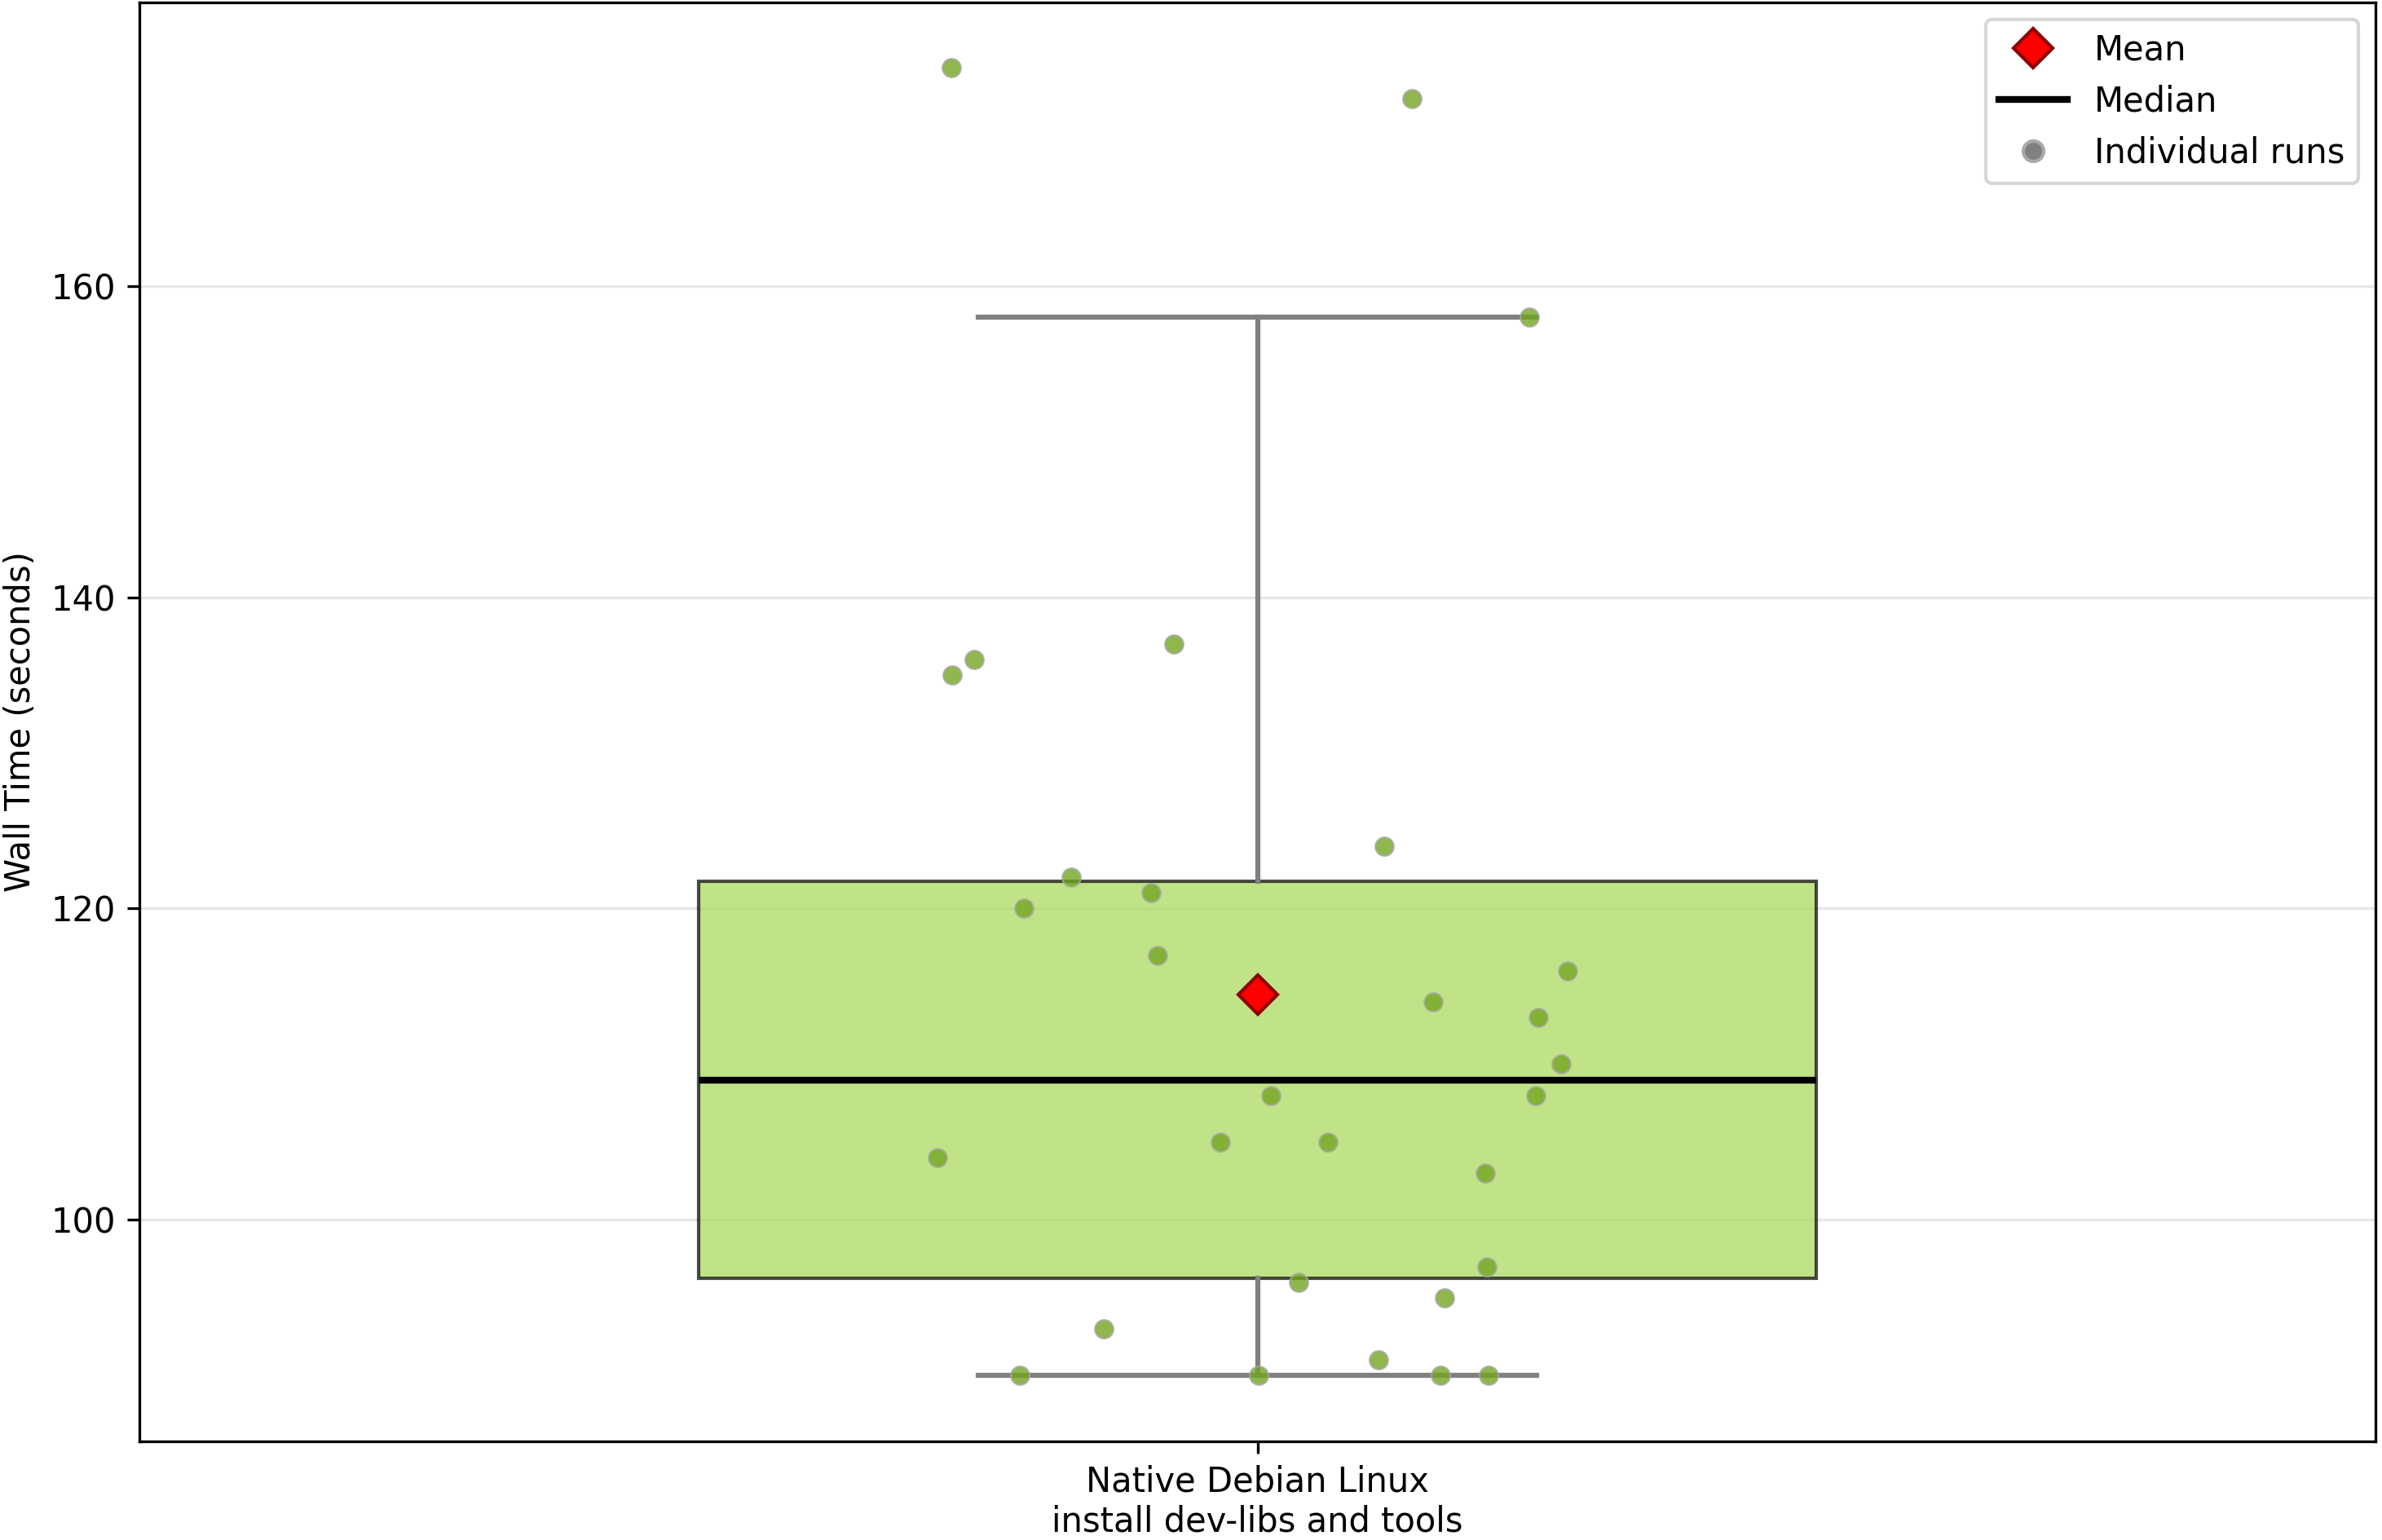
\includegraphics[width=0.8\linewidth]{figures/scenario_1_boxplot_install_devtools_wall_time.png}
    \caption{Native Linux development tools installation time distribution (n=30)}
    \label{fig:native_linux_devtools}
\end{figure}

Native Linux development tools installation completes in a median of 109 seconds with notably higher variance (standard deviation of 22.99 seconds) compared to other operations.
This variance stems from package manager behavior, including dependency resolution, mirror selection, and download speeds.
The skewed distribution (median of 109s vs.\ mean of 114s) indicates occasional slow runs that pull the average upward.

\subsection{Comparative analysis: Toolchain switching}
\label{subsec:toolchain_switching_comparison}

Figure~\ref{fig:scenario1_total_runtime} visualizes the total runtime distribution for complete toolchain switching operations across all environments, and Table~\ref{tab:toolchain_switching_comparison} presents the comprehensive statistical comparison.

\begin{figure}[htbp]
    \centering
    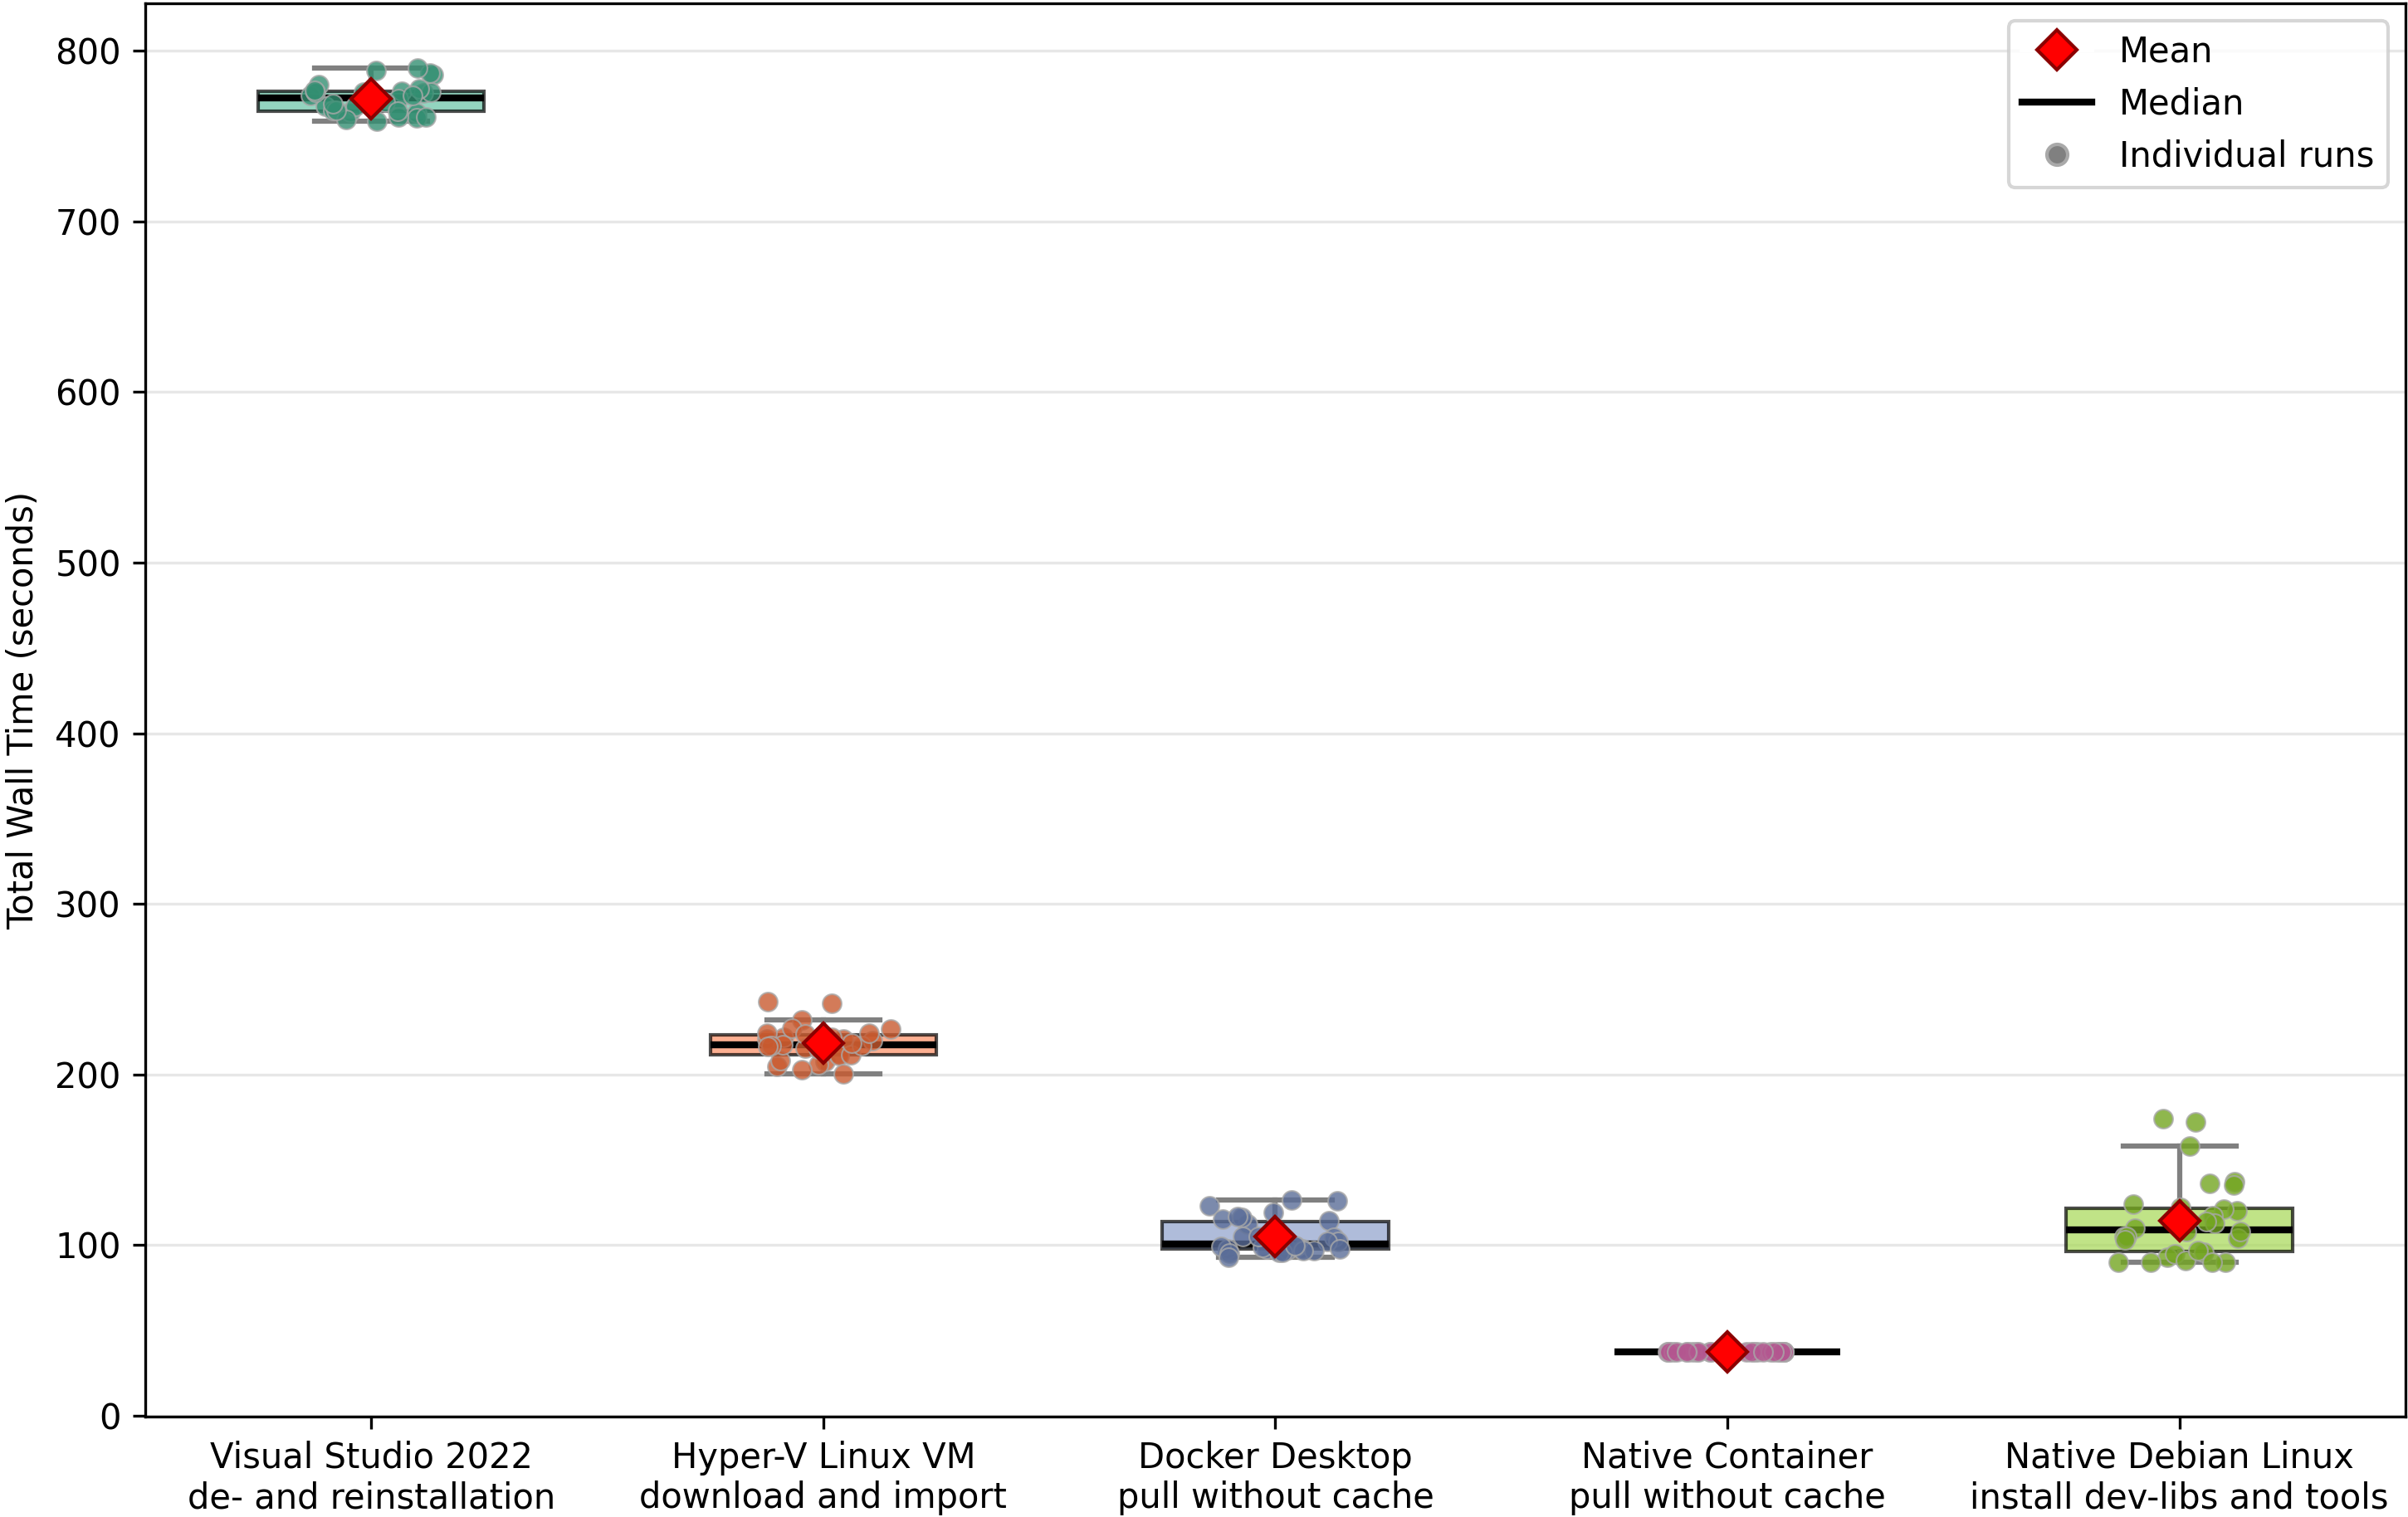
\includegraphics[width=\linewidth]{figures/scenario_1_boxplot_total_runtime.png}
    \caption{Total runtime distribution for toolchain switching by environment (n=30)}
    \label{fig:scenario1_total_runtime}
\end{figure}

\begin{table}[htbp]
    \centering
    \begin{tabular}{|l|c|c|c|c|c|c|}
        \hline
        \textbf{Environment} & \textbf{Mean (s)} & \textbf{Median (s)} & \textbf{Std Dev} & \textbf{Min (s)} & \textbf{Max (s)} & \textbf{Reduction} \\
        \hline
        Native Windows (VS2022) & 771.75 & 772.25 & 8.77 & 758.69 & 789.92 & baseline \\
        Native Linux (devtools) & 114.47 & 109.00 & 22.99 & 90.00 & 174.00 & $-$85.9\% \\
        Hyper-V VM & 218.18 & 217.48 & 9.99 & 200.53 & 242.73 & $-$71.8\% \\
        Docker Desktop (WSL2) & 105.00 & 100.78 & 10.02 & 93.02 & 126.50 & $-$87.0\% \\
        Native Container (Linux) & 37.48 & 37.48 & 0.05 & 37.34 & 37.60 & $-$95.1\% \\
        \hline
    \end{tabular}
    \caption{Toolchain switching time comparison across environments (n=30)}
    \label{tab:toolchain_switching_comparison}
\end{table}

The results establish a clear performance hierarchy: native containers on Linux complete switching in 37.5 seconds (95.1\% faster than baseline), followed by Docker Desktop on Windows at 1.68 minutes (87.0\% faster), native Linux package installation at 1.8 minutes (85.9\% faster), Hyper-V VM switching at 3.6 minutes (71.8\% faster), and native Windows Visual Studio switching at 12.9 minutes (baseline).
Native containers show exceptional consistency (standard deviation 0.05s), while native Linux package installation exhibits the highest variance (22.99s) due to package manager behavior.

\section{Scenario 2: Comprehensive performance benchmarking}

This scenario evaluates build, installation, and test execution performance across six environments with infrastructure already provisioned.
The analysis examines real-world development workflows including CMake configuration, full builds, incremental builds with varying scopes, installation procedures, and test execution.
Measurements focus on wall-clock time, CPU utilization, and memory consumption.

Statistical significance of performance differences was evaluated using two-tailed independent samples t-tests as specified in Section~\ref{sec:methodology_evaluation}.
Pairwise comparisons between environments showed that the vast majority of observed wall-clock time differences were statistically significant at the $\alpha = 0.05$ level, with most yielding $p < 0.001$.
Complete statistical test results for all pairwise comparisons across all metrics (wall time, CPU utilization, memory consumption) are provided in Appendix~\nameref{appendix:statistical_tests}.
The following subsections focus on the magnitude and practical implications of these differences.

The six evaluated environments represent different deployment approaches:
\begin{itemize}
    \item Windows 11 native --- baseline environment using CMake/Ninja/cl.exe toolchain
    \item Hyper-V Windows 11 Guest --- virtualized Windows on Windows host
    \item Debian 12 native --- native Linux development environment
    \item Hyper-V Debian 12 Guest --- virtualized Linux on Windows host
    \item Docker Desktop on Windows 11 --- containerized Linux with volume-mounted source (WSL2 backend)
    \item Docker on Linux --- containerized Linux on native Linux host
\end{itemize}

The scenario is divided into three parts: standard build workflow benchmarks (Sections \ref{subsec:cmake_configure}--\ref{subsec:total_runtime_standard}), unit test execution analysis (Section \ref{subsec:unittest_execution}), and optimized workflow evaluation with compiler caching (Section \ref{subsec:optimized_workflow}).
Each subsection presents a specific benchmark's characteristics, statistical overview, detailed distribution analysis, and supporting visualizations.

\textbf{Note on host memory measurements:} For hypervisor-based environments (Hyper-V Windows Guest, Hyper-V Debian Guest, Docker Desktop with WSL2), ``Host Peak Mem'' columns in result tables represent the total memory allocated to the VM infrastructure by the host system, including the guest operating system.
These values substantially exceed the ``Mem $\Delta$ Peak'' measurements observed within guest environments and are not directly comparable to their native environment memory delta counterparts.
Memory allocation strategies differ by configuration: Hyper-V Debian Guest uses static 20 GB host memory allocation; Hyper-V Windows Guest and Docker Desktop with WSL2 use dynamic memory allocation to maximum 20 GB.
Docker on Linux uses native containers without a hypervisor and therefore shows no host memory overhead similarly.

\subsection{Standard build workflow benchmarks}
\label{subsec:standard_build_workflow}

The following subsections examine the core build workflow operations without compiler caching or other optimizations, establishing baseline performance characteristics for each environment.

\subsubsection{CMake configuration performance}
\label{subsec:cmake_configure}

CMake configuration represents the initial project analysis phase where CMake examines the build environment, locates compilers and dependencies, and generates build system files.
This operation is heavily I/O-bound, involving extensive filesystem operations for discovering headers, libraries, and toolchain components.

\begin{table}[htbp]
    \centering
    \footnotesize
    \begin{tabular}{|l|r|r|r|r|r|}
        \hline
        \textbf{Environment} & \textbf{Wall Time} & \textbf{vs Baseline} & \textbf{CPU $\Delta$ Mean} & \textbf{Mem $\Delta$ Peak} & \textbf{Host Peak Mem} \\
        & \textbf{Median (s)} & & \textbf{Median (\%)} & \textbf{Median (MB)} & \textbf{Median (MB)} \\
        \hline
        Win11 native & 36.69 & baseline & 5.47 & 1093.10 & --- \\
        Hyper-V Win11 & 42.37 & +15.5\% & 5.80 & 586.91 & 4728.76 \\
        Debian native & 20.92 & $-$43.0\% & 5.14 & 238.50 & --- \\
        Hyper-V Debian & 21.66 & $-$41.0\% & 5.16 & 240.01 & 20480 \\
        Docker Desktop & 23.56 & $-$35.8\% & 5.12 & 243.74 & 3964.04 \\
        Docker Linux & 21.11 & $-$42.5\% & 5.05 & 240.80 & --- \\
        \hline
    \end{tabular}
    \caption{CMake configuration performance (n=30)}
    \label{tab:cmake_configure_s2}
\end{table}

\begin{figure}[htbp]
    \centering
    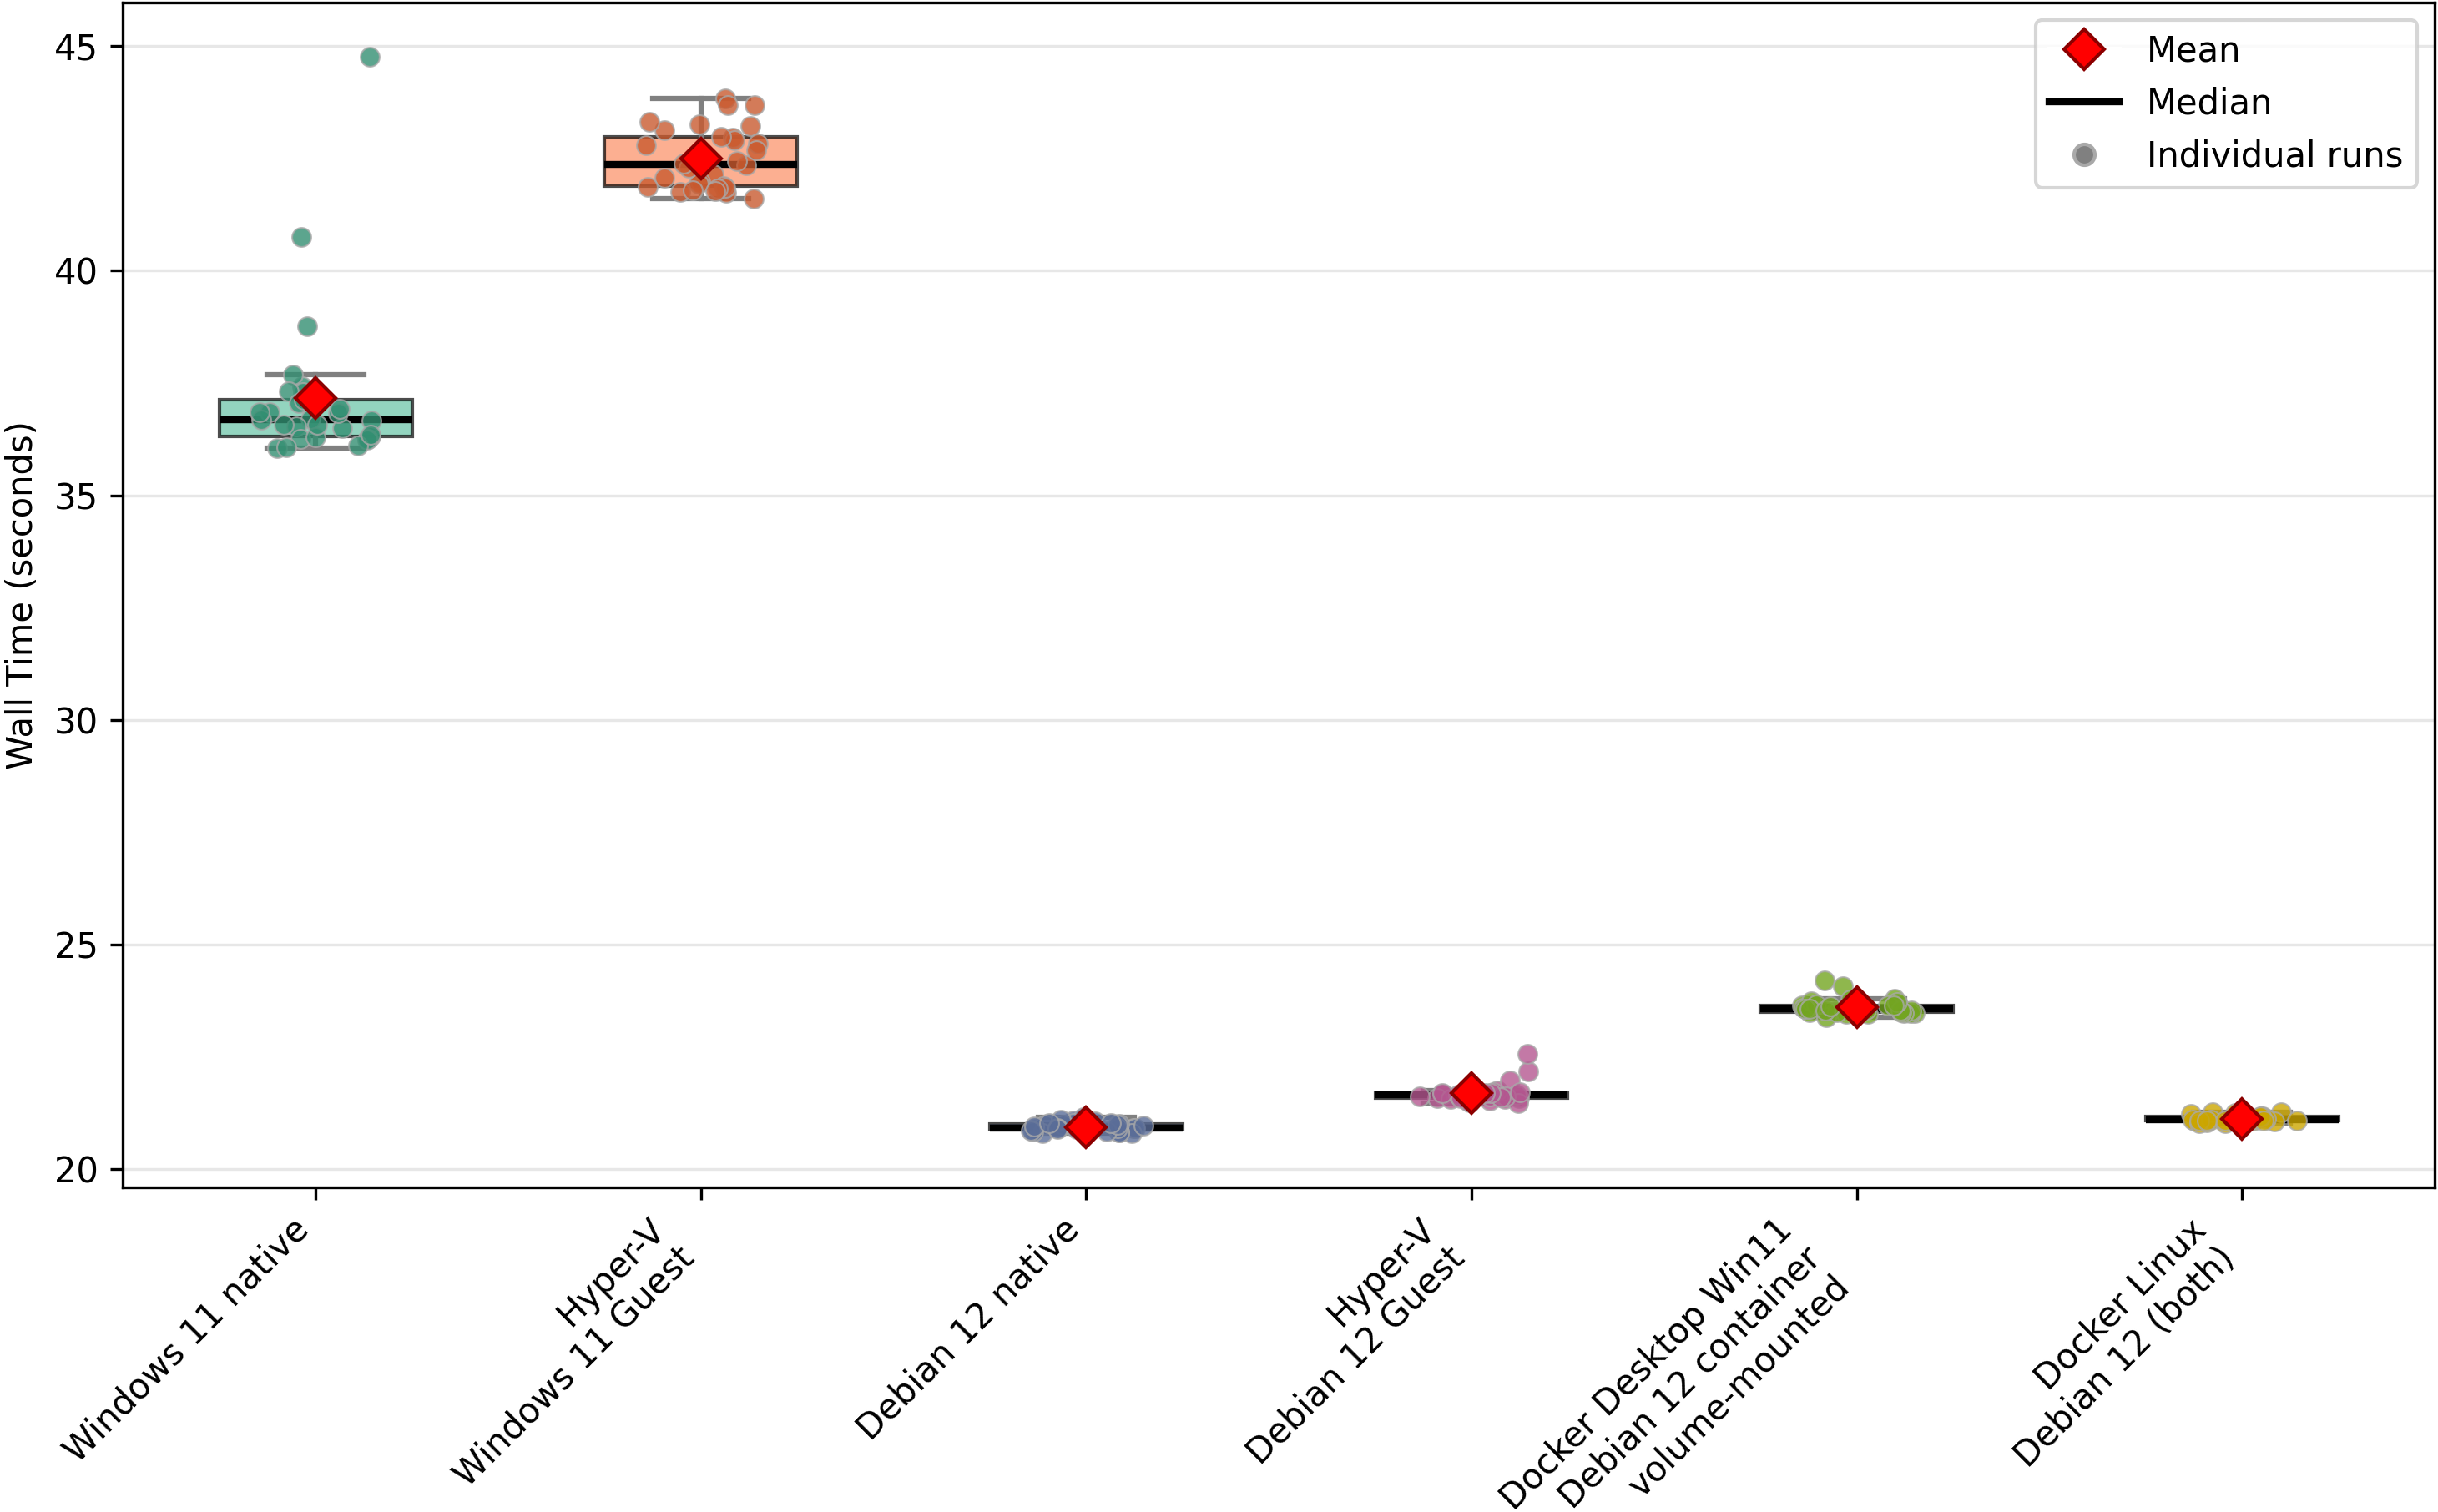
\includegraphics[width=\linewidth]{figures/scenario_2_boxplot_cmake_configure_wall_time.png}
    \caption{CMake configuration wall time distribution across environments (n=30)}
    \label{fig:cmake_configure_wall_time}
\end{figure}

The results reveal a clear performance divide between Windows and Linux environments.
All Linux-based configurations---native, virtualized, and containerized---complete CMake configuration 35--43\% faster than the Windows baseline, with median times clustering tightly between 20.92 and 23.56 seconds.
In contrast, Windows environments require 36.69--42.37 seconds, with Hyper-V adding 15.5\% overhead to the already slower Windows baseline.
The low CPU utilization across all environments (5--6\%) confirms this workload's I/O-bound nature, dominated by filesystem operations for header discovery, dependency resolution, and build file generation.

Memory consumption patterns in the execution environment similarly distinguish the two operating system families.
Linux-based environments exhibit consistently low memory deltas in the 238--244 MB range, while Windows environments require 587--1093 MB.
Host-side memory measurements for hypervisor-based environments (4.0--4.7 GB) reflect total infrastructure allocation including the guest OS.

Linux-based approaches also demonstrate high consistency.
Debian native achieves a standard deviation of just 0.09 seconds (Q1: 20.89s, Q3: 21.00s), and Docker Desktop shows similarly tight clustering at 0.18 seconds.
Windows native exhibits higher variability (standard deviation: 1.71 seconds), with outliers reaching up to 43.60 seconds compared to the median of 36.69 seconds, suggesting interference from background Windows services or filesystem operations.

\subsubsection{Clean build performance}
\label{subsec:clean_build}

A clean build compiles the entire codebase from scratch, representing the maximum compilation workload.
This benchmark measures CPU-bound compilation performance, as all source files must be parsed, compiled, and linked without leveraging any cached artifacts.

\begin{table}[htbp]
    \centering
    \footnotesize
    \begin{tabular}{|l|r|r|r|r|r|}
        \hline
        \textbf{Environment} & \textbf{Wall Time} & \textbf{vs Baseline} & \textbf{CPU $\Delta$ Mean} & \textbf{Mem $\Delta$ Peak} & \textbf{Host Peak Mem} \\
        & \textbf{Median (s)} & & \textbf{Median (\%)} & \textbf{Median (MB)} & \textbf{Median (MB)} \\
        \hline
        Win11 native & 1003.89 & baseline & 99.38 & 8595.53 & --- \\
        Hyper-V Win11 & 1106.19 & +10.2\% & 99.27 & 8009.67 & 13396.80 \\
        Debian native & 930.17 & $-$7.3\% & 99.53 & 9643.26 & --- \\
        Hyper-V Debian & 1000.40 & $-$0.3\% & 99.62 & 9628.61 & 20480 \\
        Docker Desktop & 1150.11 & +14.6\% & 99.61 & 9497.87 & 19996.12 \\
        Docker Linux & 931.30 & $-$7.2\% & 99.55 & 9671.71 & --- \\
        \hline
    \end{tabular}
    \caption{Clean build performance (n=30)}
    \label{tab:cmake_build_full_s2}
\end{table}

\begin{figure}[htbp]
    \centering
    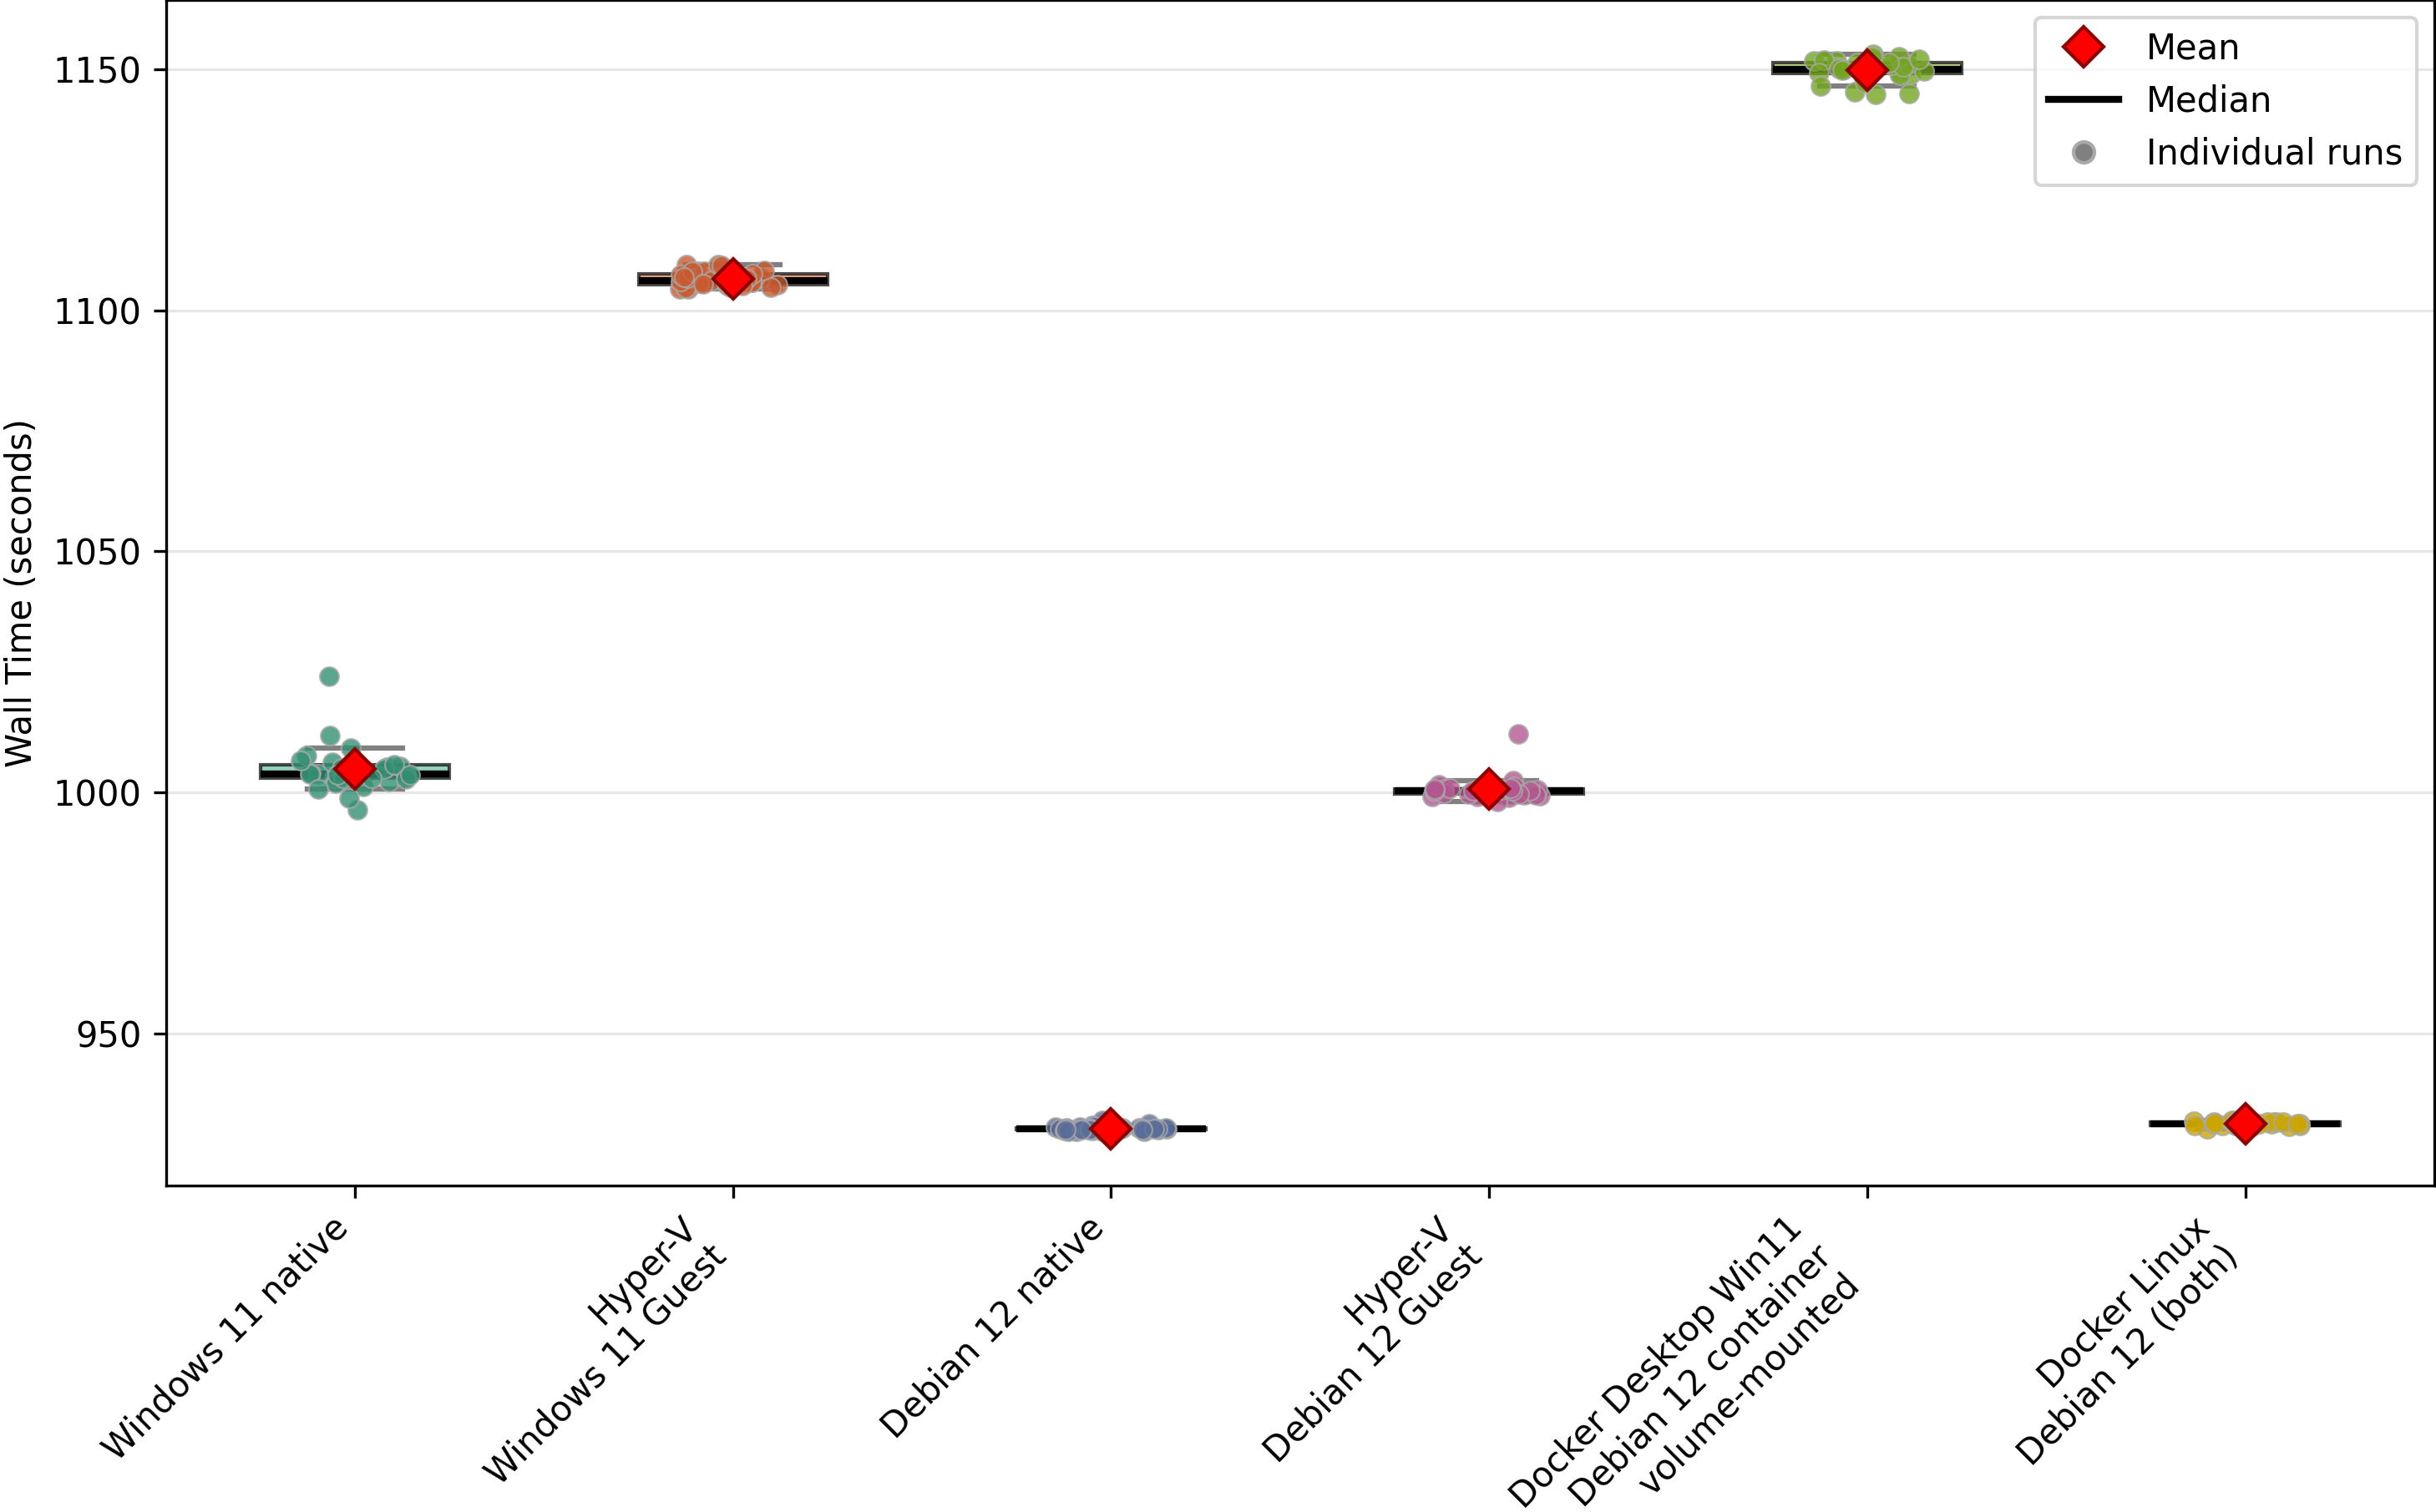
\includegraphics[width=\linewidth]{figures/scenario_2_boxplot_cmake_build_full_wall_time.png}
    \caption{Clean build wall time distribution across environments (n=30)}
    \label{fig:cmake_build_full_wall_time}
\end{figure}

Debian native achieves a median build time of 930.17 seconds, representing a 7.3\% improvement over the Windows native baseline of 1003.89 seconds.
Docker on Linux performs nearly identically at 931.30 seconds (7.2\% faster than baseline), demonstrating minimal containerization overhead for CPU-intensive workloads.
Hyper-V Debian Guest completes in 1000.40 seconds, essentially matching Windows native performance with only 0.3\% slower execution.

Windows-based containerization imposes a notable penalty: Docker Desktop requires 1150.11 seconds (14.6\% slower than baseline), while Hyper-V Windows Guest requires 1106.19 seconds (10.2\% slower).
These overheads stem from the WSL2 virtualization layer required for Docker Desktop on Windows and the Hyper-V hypervisor overhead.

CPU utilization exceeds 99\% across all environments, confirming this workload's CPU-bound nature and saturating available CPU cores with parsing, optimization, and code generation tasks.

System memory consumption ranges from 8.0--9.7 GB delta from baseline across all platforms.
Debian-based environments show approximately 1 GB higher system memory deltas than Windows environments.
Host-side memory for hypervisor-based environments ranges from 13.4--20.0 GB, including guest OS overhead.

Linux-based environments demonstrate higher consistency: Debian native and Docker Linux achieve standard deviations of 0.47 and 0.45 seconds respectively.
Docker Desktop shows slightly higher variability (2.22 seconds), while Windows native exhibits the highest variation (4.66 seconds), though all environments maintain stable performance for this compute-intensive workload.

\subsubsection{Installation workflow performance}
\label{subsec:installation_workflow}

This benchmark measures the CMake installation process, copying built artifacts to their final installation directories, which is heavily I/O-bound involving file copying and directory creation operations.

\begin{table}[ht]
    \centering
    \footnotesize
    \begin{tabular}{|l|r|r|r|r|r|}
        \hline
        \textbf{Environment} & \textbf{Wall Time} & \textbf{vs Baseline} & \textbf{CPU $\Delta$ Mean} & \textbf{Mem $\Delta$ Peak} & \textbf{Host Peak Mem} \\
        & \textbf{Median (s)} & & \textbf{Median (\%)} & \textbf{Median (MB)} & \textbf{Median (MB)} \\
        \hline
        Win11 native & 21.80 & baseline & 5.73 & 1713.24 & --- \\
        Hyper-V Win11 & 44.06 & +102.1\% & 4.97 & 1227.50 & 12725.22 \\
        Debian native & 5.90 & $-$72.9\% & 5.46 & 46.28 & --- \\
        Hyper-V Debian & 15.05 & $-$31.0\% & 3.05 & 31.16 & 20480 \\
        Docker Desktop & 16.09 & $-$26.2\% & 3.70 & 130.24 & 19937.54 \\
        Docker Linux & 6.10 & $-$72.0\% & 5.35 & 39.53 & --- \\
        \hline
    \end{tabular}
    \caption{Installation workflow performance (n=30)}
    \label{tab:cmake_build_install_s2}
\end{table}

\begin{figure}[ht]
    \centering
    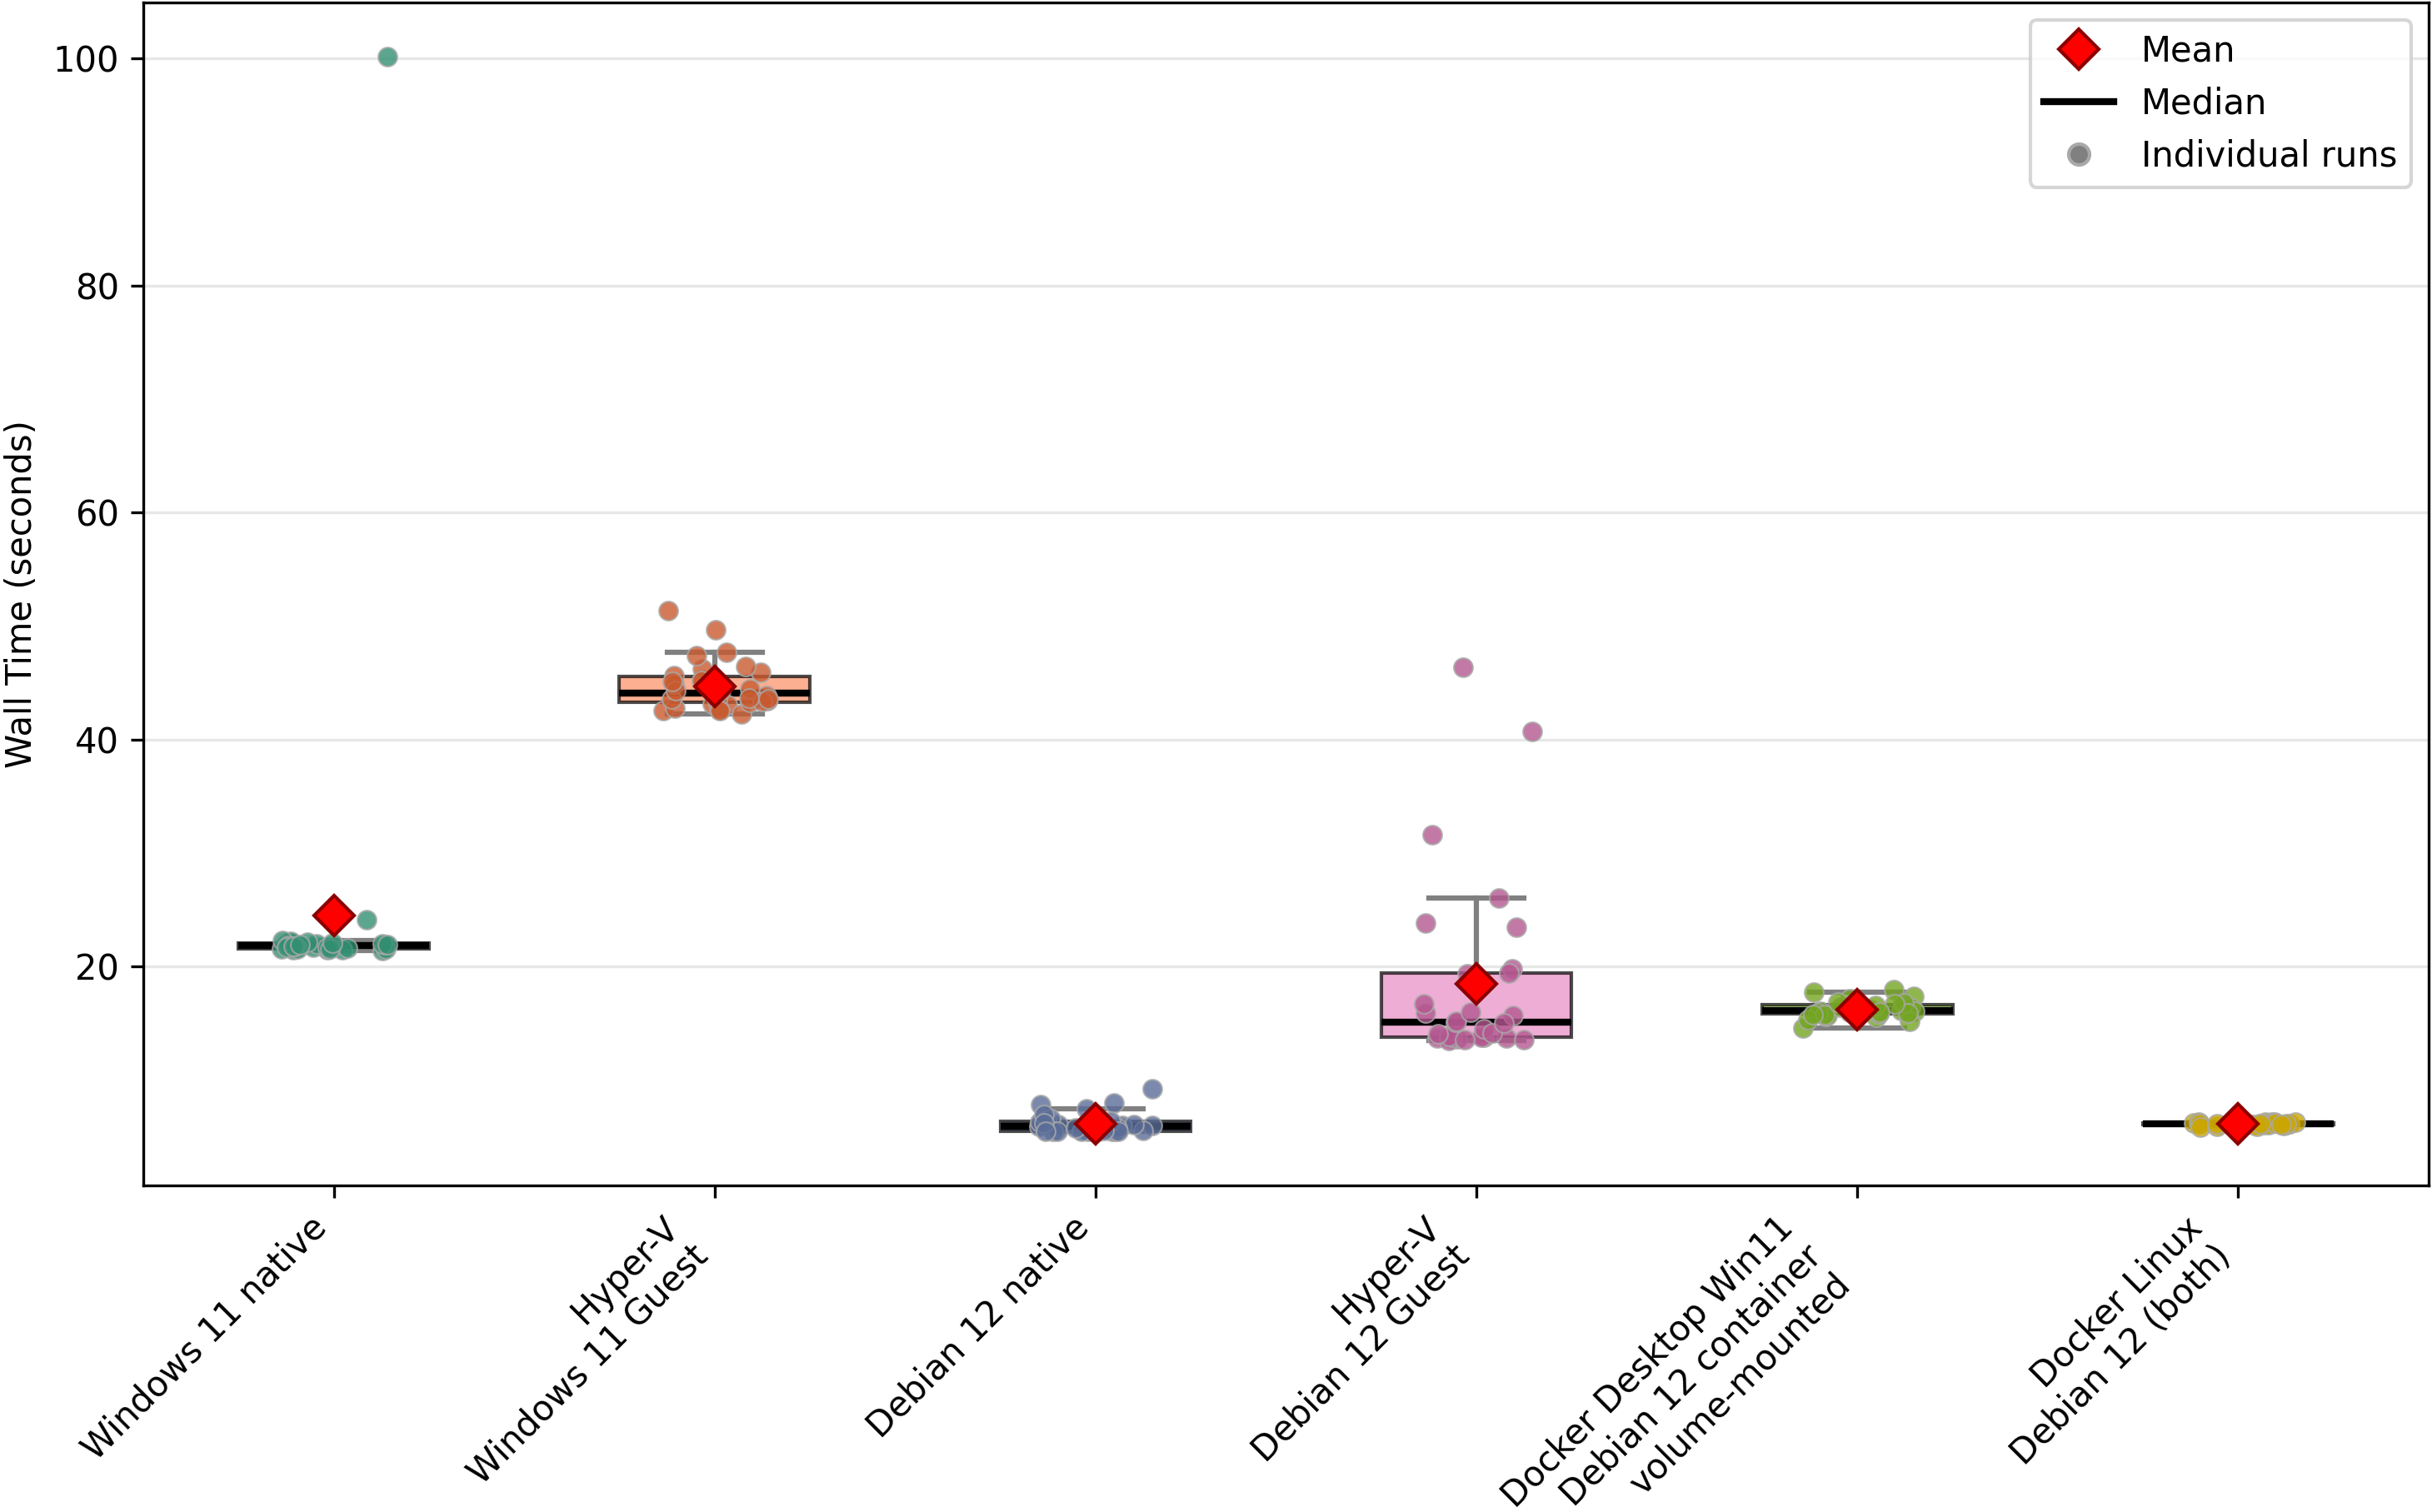
\includegraphics[width=\linewidth]{figures/scenario_2_boxplot_cmake_build_install_wall_time.png}
    \caption{Installation workflow wall time distribution across environments (n=30)}
    \label{fig:cmake_build_install_wall_time}
\end{figure}

This benchmark exhibits the highest variability across all measured operations.
Linux environments achieve the fastest installation times: Debian native completes in 5.90 seconds and Docker on Linux in 6.10 seconds, both approximately 72\% faster than the Windows baseline.
Docker Desktop on Windows (16.09 seconds) outperforms Windows native (21.80 seconds) despite containerization overhead.

Windows native shows considerable variance (mean: 24.49s, standard deviation: 14.31s) with outliers reaching up to 100 seconds, suggesting occasional interference from filesystem operations, antivirus scanning, or system services.
Hyper-V Windows Guest requires 44.06 seconds median (102.1\% slower than baseline) with more consistent behavior (standard deviation: 2.16s), while Hyper-V Debian Guest shows elevated variance (standard deviation: 8.15s) with some runs extending to 46 seconds due to disk I/O virtualization overhead.

The low CPU utilization (3--6\% across all environments) confirms this workload's I/O-bound nature, dominated by file copying operations.
System memory consumption remains minimal across Linux environments (31--46 MB delta median), while Windows native shows higher system memory delta (1713.24 MB).
Host-side memory measurements (12.7--19.9 GB) reflect residual allocations from the preceding clean build operation in the benchmark sequence.

These results indicate that installation performance is particularly sensitive to filesystem implementation and I/O subsystem architecture, with Linux-based environments consistently outperforming Windows for file installation workflows.

\subsubsection{Incremental build: New CMake target}
\label{subsec:incremental_new_target}

This benchmark evaluates incremental build performance when adding a new CMake target (executable or library) to the project.
The operation requires CMake reconfiguration to process the new target definition, followed by compilation and linking of the new component.
This represents a common development workflow when extending a project with new modules or executables.

\begin{table}[htbp]
    \centering
    \footnotesize
    \begin{tabular}{|l|r|r|r|r|r|}
        \hline
        \textbf{Environment} & \textbf{Wall Time} & \textbf{vs Baseline} & \textbf{CPU $\Delta$ Mean} & \textbf{Mem $\Delta$ Peak} & \textbf{Host Peak Mem} \\
        & \textbf{Median (s)} & & \textbf{Median (\%)} & \textbf{Median (MB)} & \textbf{Median (MB)} \\
        \hline
        Win11 native & 13.90 & baseline & 13.09 & 1199.35 & --- \\
        Hyper-V Win11 & 20.73 & +49.1\% & 10.73 & 1209.64 & 4780.91 \\
        Debian native & 5.28 & $-$62.0\% & 15.65 & 1355.05 & --- \\
        Hyper-V Debian & 5.99 & $-$56.9\% & 15.66 & 1449.72 & 20480 \\
        Docker Desktop & 7.25 & $-$47.8\% & 14.25 & 1502.24 & 3792.51 \\
        Docker Linux & 5.61 & $-$59.6\% & 15.01 & 1386.90 & --- \\
        \hline
    \end{tabular}
    \caption{Incremental build performance for new CMake target (n=30)}
    \label{tab:cmake_build_incremental_feature_s2}
\end{table}

\begin{figure}[htbp]
    \centering
    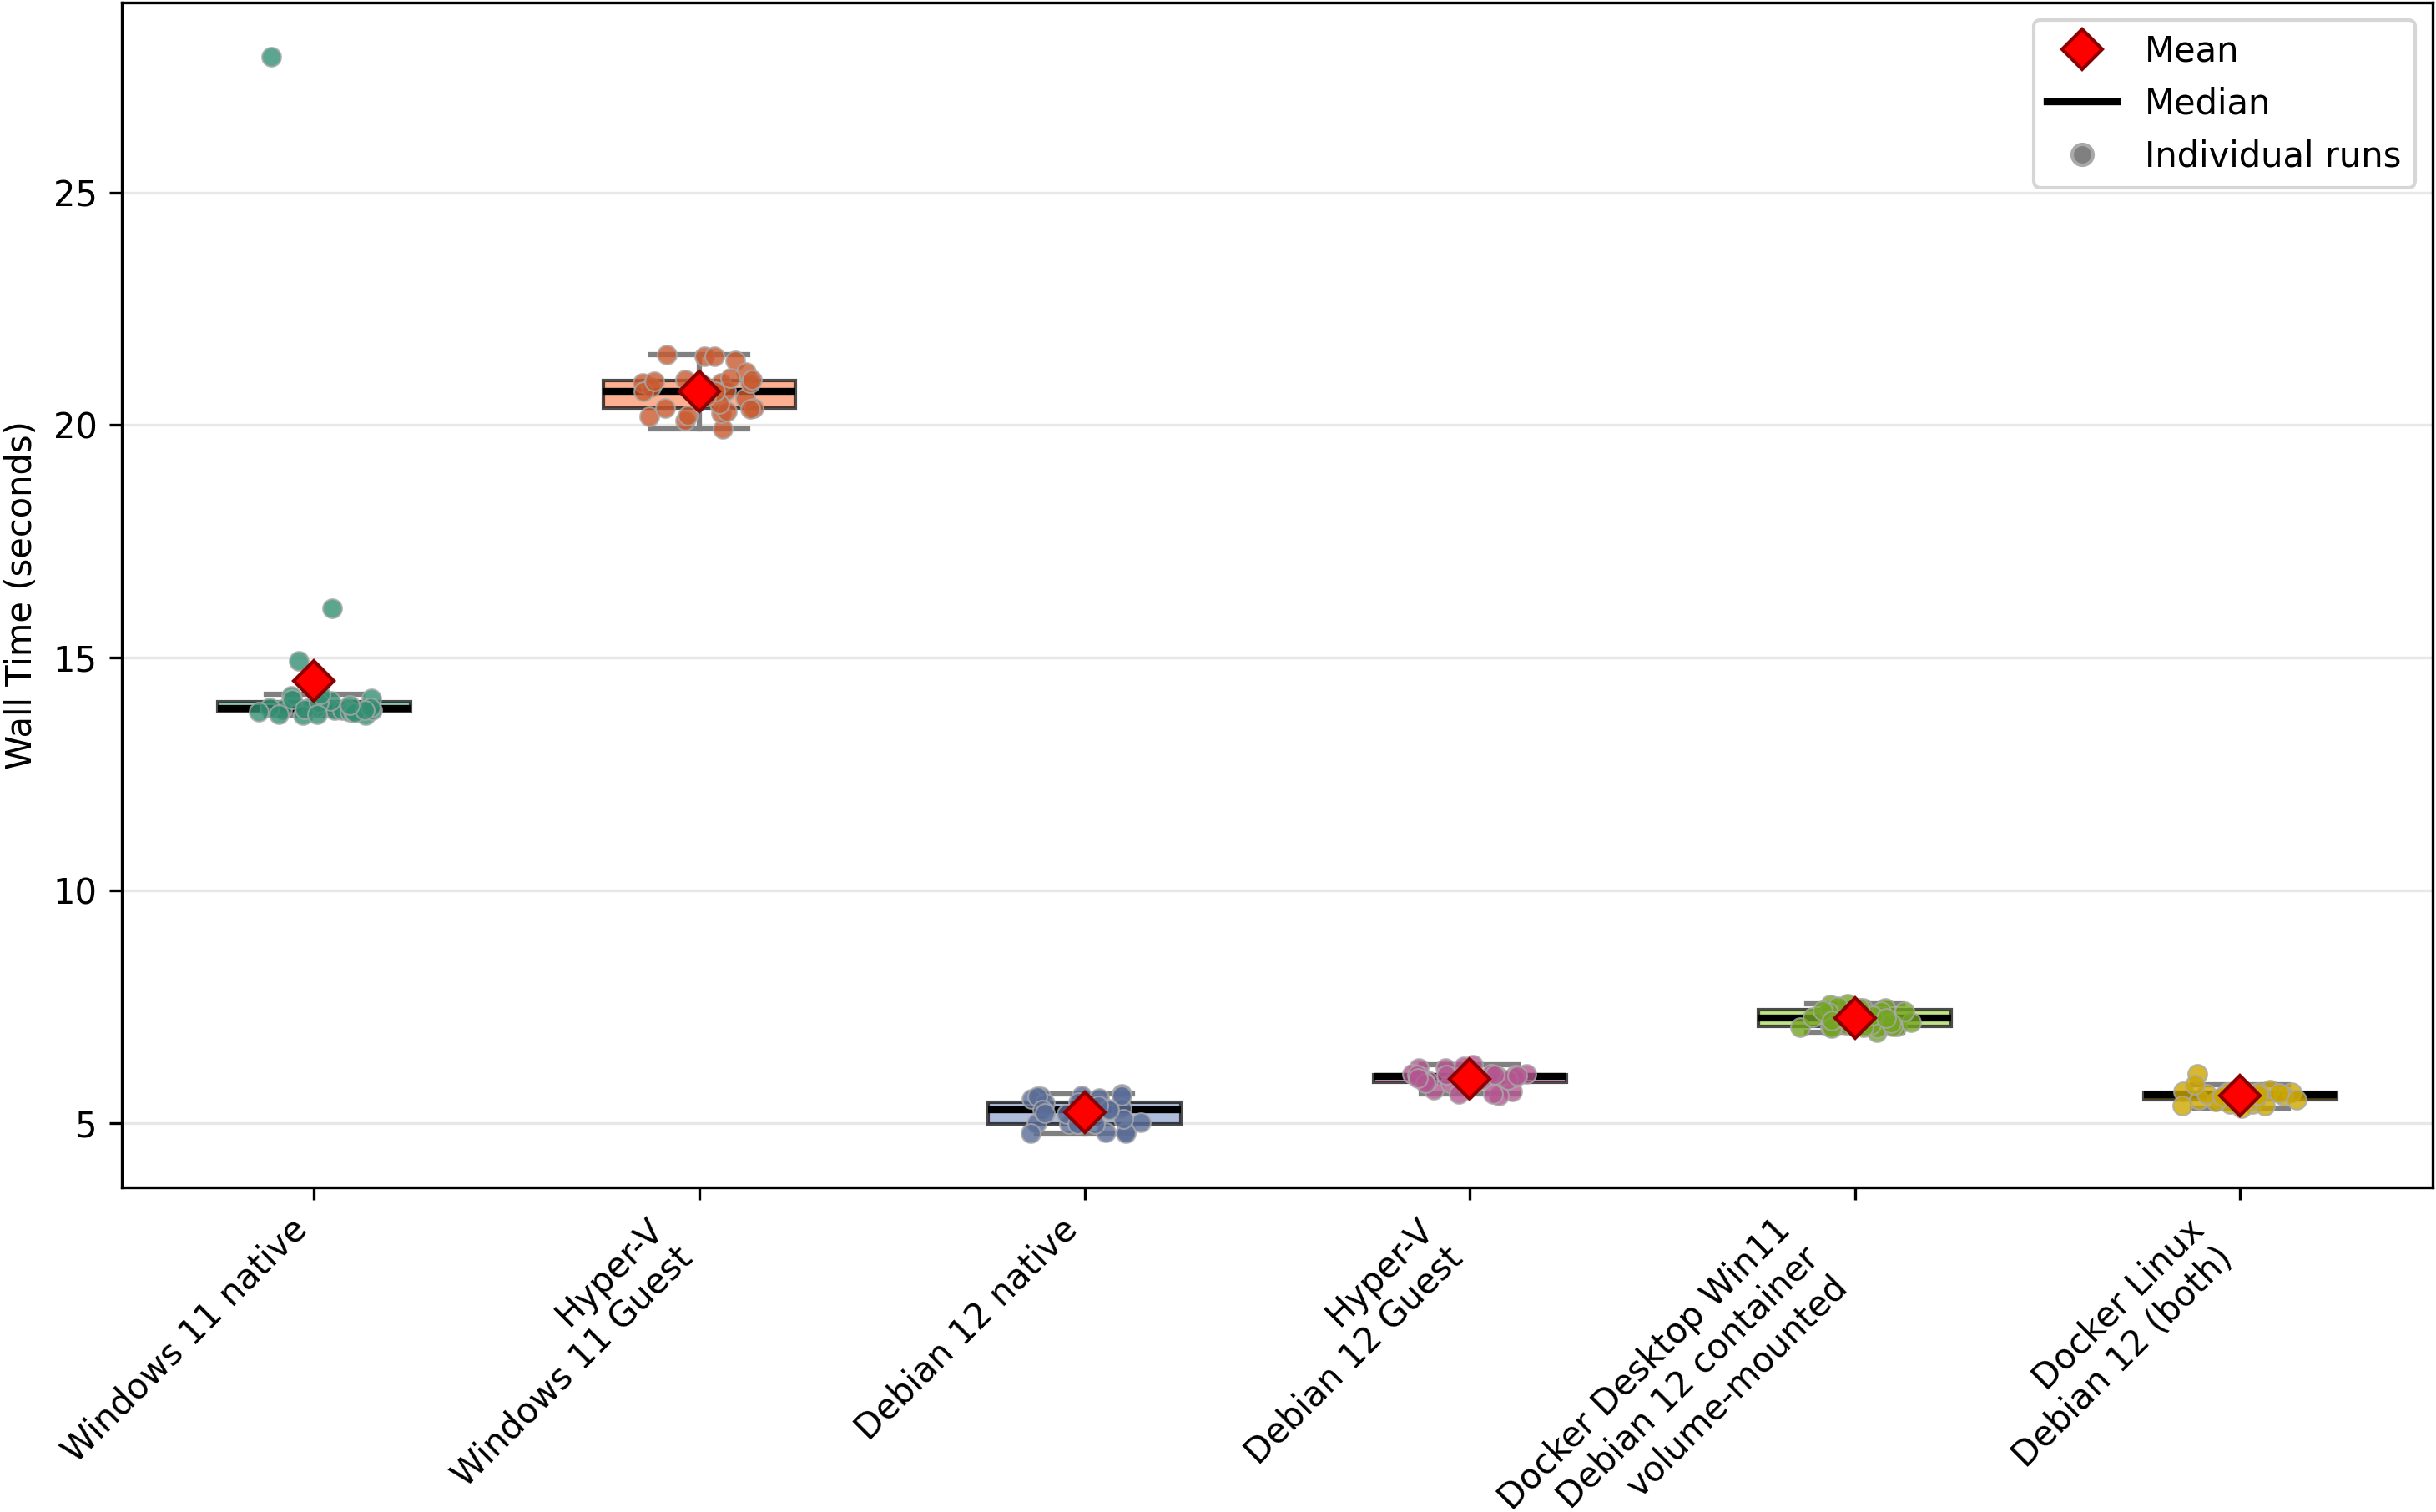
\includegraphics[width=\linewidth]{figures/scenario_2_boxplot_cmake_build_incremental_feature_wall_time.png}
    \caption{Incremental build (new target) wall time distribution across environments (n=30)}
    \label{fig:cmake_build_incremental_feature_wall_time}
\end{figure}

This benchmark shows notable performance differences between Windows and Linux environments.
Linux-based environments consistently outperform Windows: Debian native completes builds in 5.28 seconds (62.0\% faster than the Windows baseline of 13.90 seconds), Docker on Linux achieves 5.61 seconds (59.6\% faster), and Hyper-V Debian requires 5.99 seconds (56.9\% faster).
Docker Desktop on Windows reaches 7.25 seconds (47.8\% faster), indicating that even volume-mounted containerized workflows provide benefits for I/O-intensive incremental builds.
In contrast, Hyper-V Windows Guest increases build time to 20.73 seconds (49.1\% slower than baseline).

The low CPU utilization (10--16\% across environments) indicates an I/O-bound workload dominated by filesystem operations for dependency checking, build artifact management, and incremental compilation orchestration.
Windows native demonstrates notably higher variance with a standard deviation of 2.57 seconds and occasional outliers (P99: 24.49s vs median 13.90s), suggesting periodic slowdowns potentially caused by Windows Defender filesystem scanning, indexing services, or other background processes.
In contrast, Linux environments maintain high consistency: Debian native shows a standard deviation of 0.27 seconds, and Docker Desktop achieves 0.18 seconds.

System memory consumption remains modest across all environments, with median deltas ranging from 1199--1502 MB.

\subsubsection{Incremental build: Single file modification}
\label{subsec:incremental_single_file}

This benchmark measures the minimal incremental build scenario: modifying a single source file and recompiling only the affected translation unit and relinking.
This represents the most frequent developer workflow during iterative development and debugging.

\begin{table}[htbp]
    \centering
    \footnotesize
    \begin{tabular}{|l|r|r|r|r|r|}
        \hline
        \textbf{Environment} & \textbf{Wall Time} & \textbf{vs Baseline} & \textbf{CPU $\Delta$ Mean} & \textbf{Mem $\Delta$ Peak} & \textbf{Host Peak Mem} \\
        & \textbf{Median (s)} & & \textbf{Median (\%)} & \textbf{Median (MB)} & \textbf{Median (MB)} \\
        \hline
        Win11 native & 4.61 & baseline & 13.09 & 398.63 & --- \\
        Hyper-V Win11 & 4.77 & +3.5\% & 10.73 & 440.54 & 4842.06 \\
        Debian native & 1.28 & $-$72.2\% & 15.65 & 330.95 & --- \\
        Hyper-V Debian & 1.37 & $-$70.3\% & 15.66 & 336.59 & 20480 \\
        Docker Desktop & 1.57 & $-$66.0\% & 14.25 & 338.82 & 2697.76 \\
        Docker Linux & 1.30 & $-$71.8\% & 15.01 & 339.40 & --- \\
        \hline
    \end{tabular}
    \caption{Incremental build performance for single file modification (n=30)}
    \label{tab:cmake_build_incremental_singlefile_s2}
\end{table}

\begin{figure}[htbp]
    \centering
    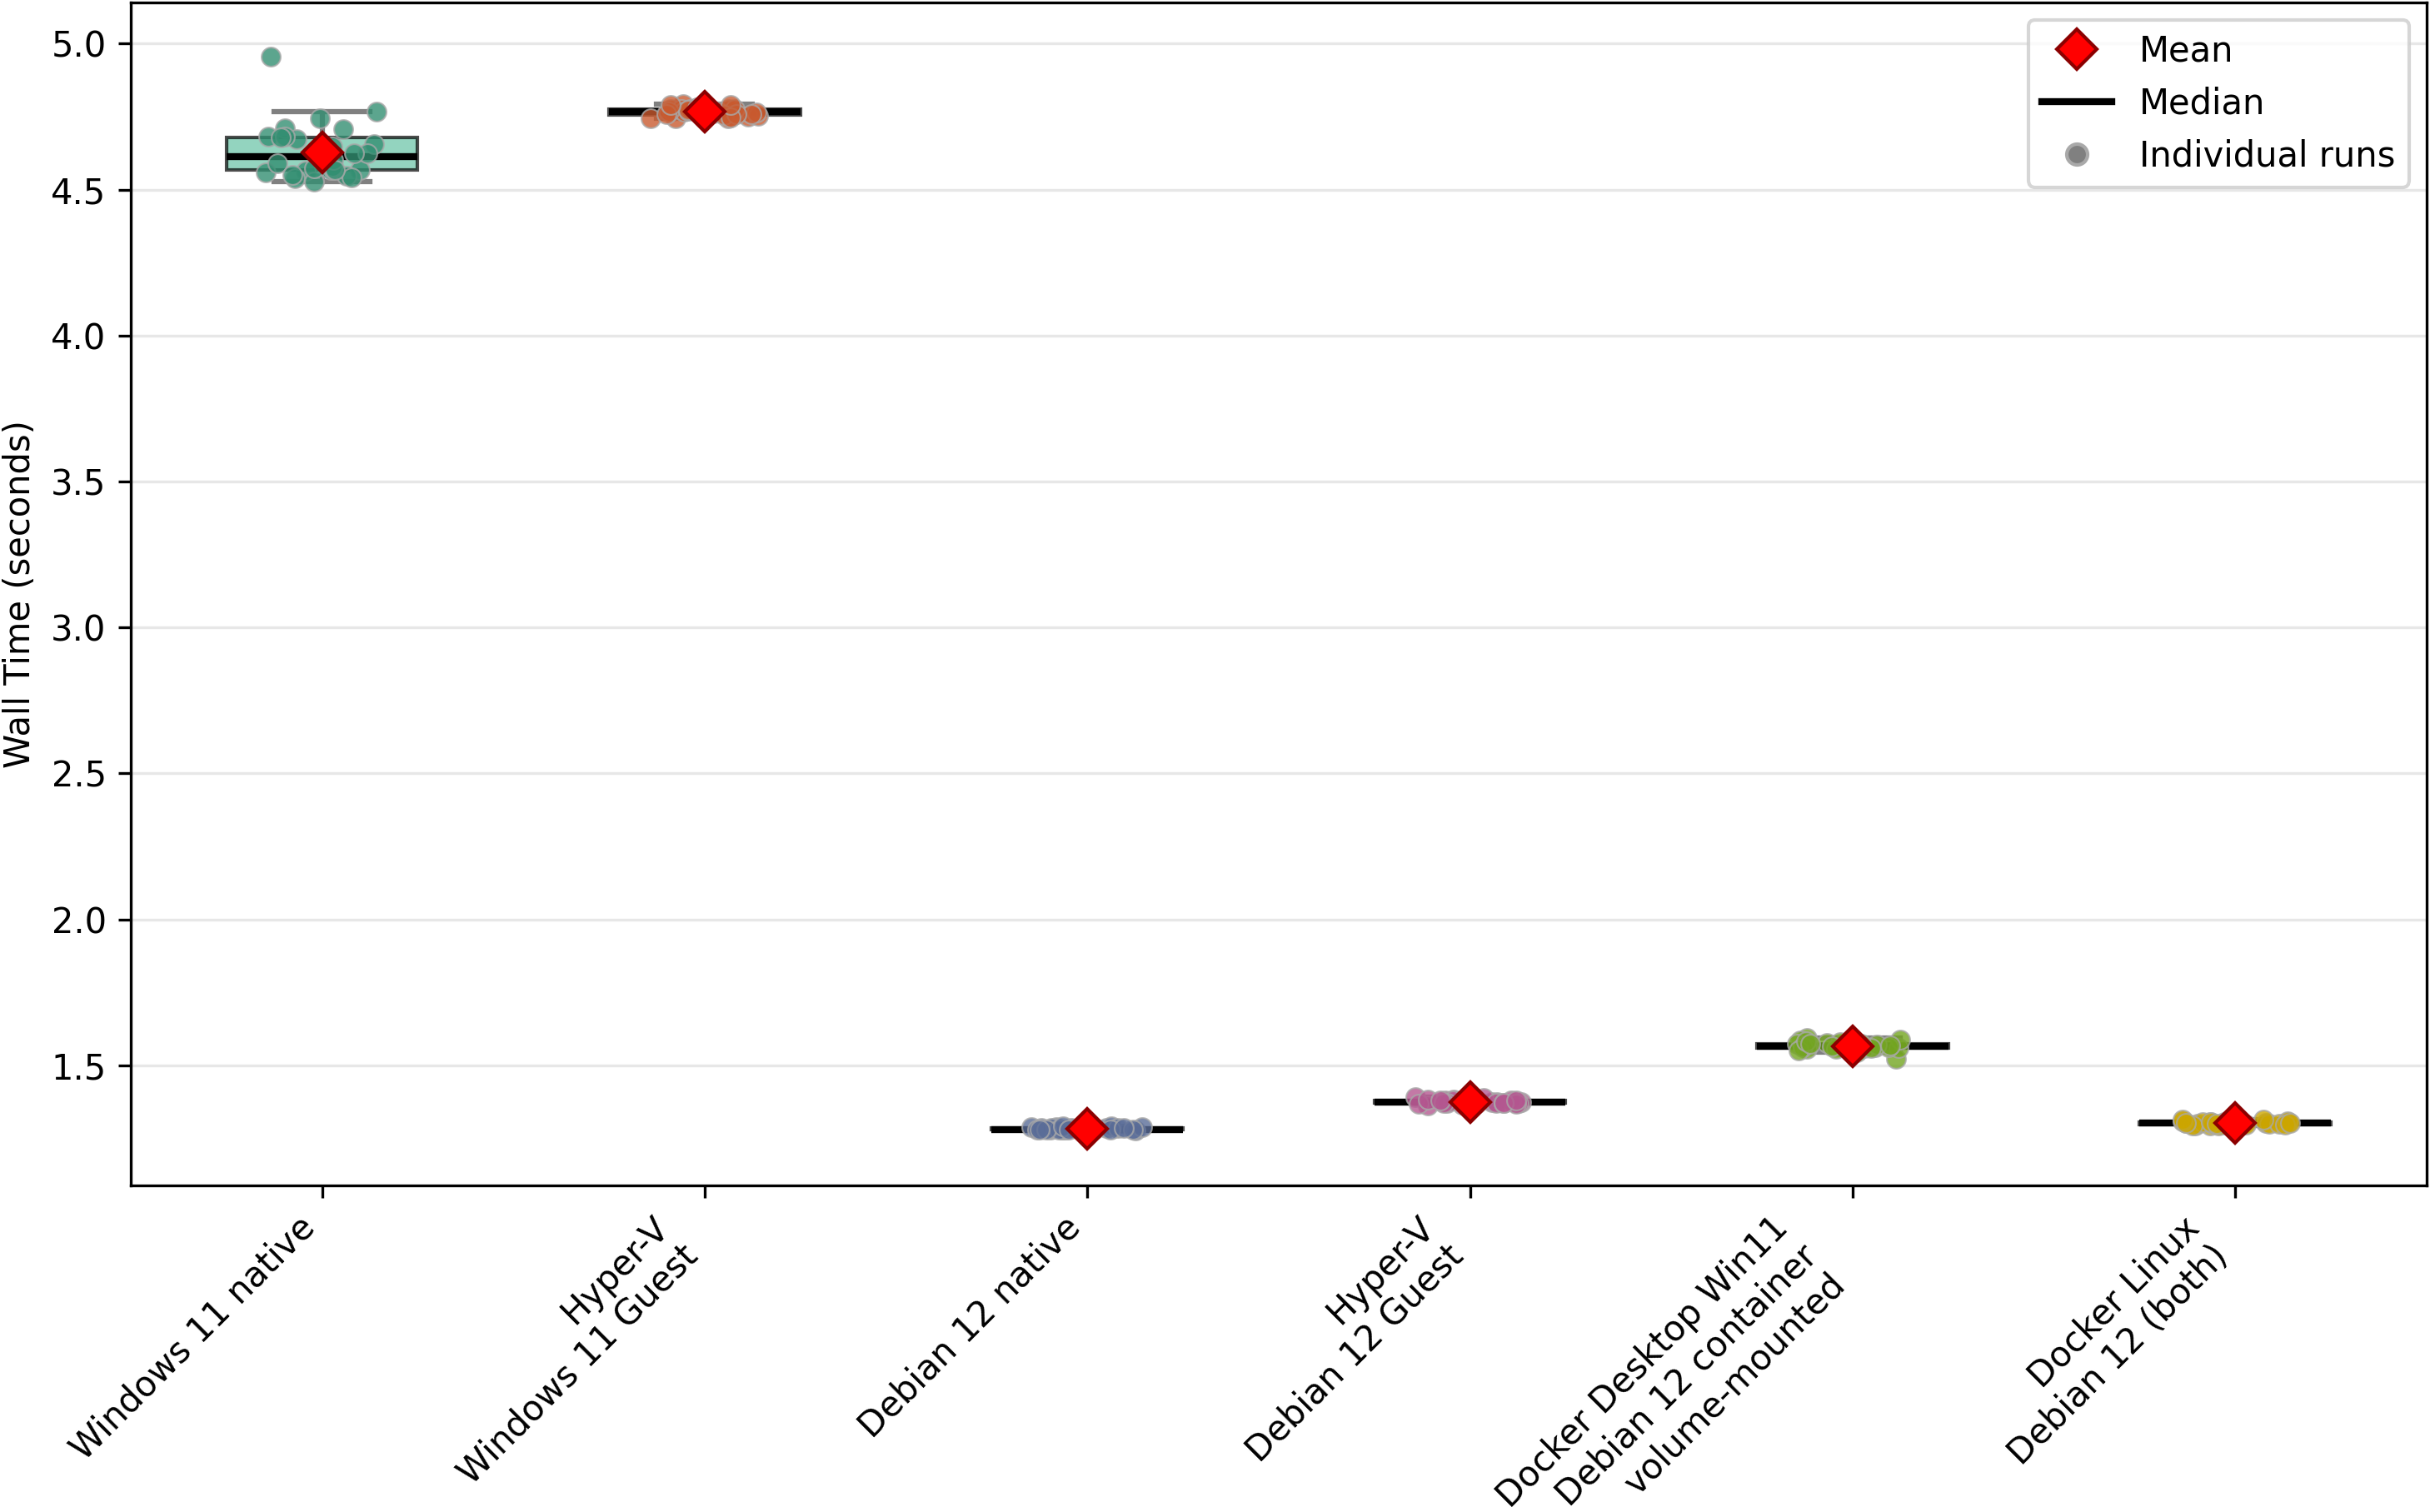
\includegraphics[width=\linewidth]{figures/scenario_2_boxplot_cmake_build_incremental_singlefile_wall_time.png}
    \caption{Incremental build (single file) wall time distribution across environments (n=30)}
    \label{fig:cmake_build_incremental_singlefile_wall_time}
\end{figure}

This shortest benchmark operation shows the largest relative performance gap between Windows and Linux environments.
Linux-based environments complete the single-file incremental build in approximately 1.3 seconds (Debian native: 1.28s, Docker Linux: 1.30s, Hyper-V Debian: 1.37s, Docker Desktop: 1.57s), representing 66--72\% improvements over the Windows native baseline of 4.61 seconds.
Windows environments require substantially longer: 4.61 seconds natively and 4.77 seconds under Hyper-V (+3.5\%).
The similarity between Windows native and Hyper-V Windows suggests the overhead stems from Windows filesystem implementation rather than virtualization.

The low CPU utilization (below 16\% across all environments) confirms this workload's I/O-bound nature, dominated by dependency checking, timestamp comparison, and build artifact management.
All environments show high consistency with standard deviations below 0.1 seconds, reflecting the deterministic nature of single-file compilation.

The nearly 4$\times$ performance difference between Windows and Linux for this operation suggests fundamental differences in filesystem performance for operations involving frequent metadata access.
Docker Desktop's 1.57-second median demonstrates that containerized Linux environments on Windows can substantially improve build times for rapid edit-compile-test cycles, despite the WSL2 virtualization layer.

\subsubsection{Total runtime: Standard workflow}
\label{subsec:total_runtime_standard}

This aggregate benchmark measures the cumulative time for executing all individual benchmarks in sequence: configuration, full build, incremental builds (both variants), and installation.
It represents the total time investment for a complete development workflow cycle without compiler caching.

\begin{table}[htbp]
    \centering
    \footnotesize
    \begin{tabular}{|l|r|r|}
        \hline
        \textbf{Environment} & \textbf{Wall Time (Median, s)} & \textbf{vs Baseline} \\
        \hline
        Win11 native & 1081.22 & baseline \\
        Hyper-V Win11 & 1218.50 & +12.7\% \\
        Debian native & 963.62 & $-$10.9\% \\
        Hyper-V Debian & 1044.67 & $-$3.4\% \\
        Docker Desktop & 1198.40 & +10.8\% \\
        Docker Linux & 965.47 & $-$10.7\% \\
        \hline
    \end{tabular}
    \caption{Total runtime for complete development workflow (n=30)}
    \label{tab:total_runtime_s2}
\end{table}

\begin{figure}[htbp]
    \centering
    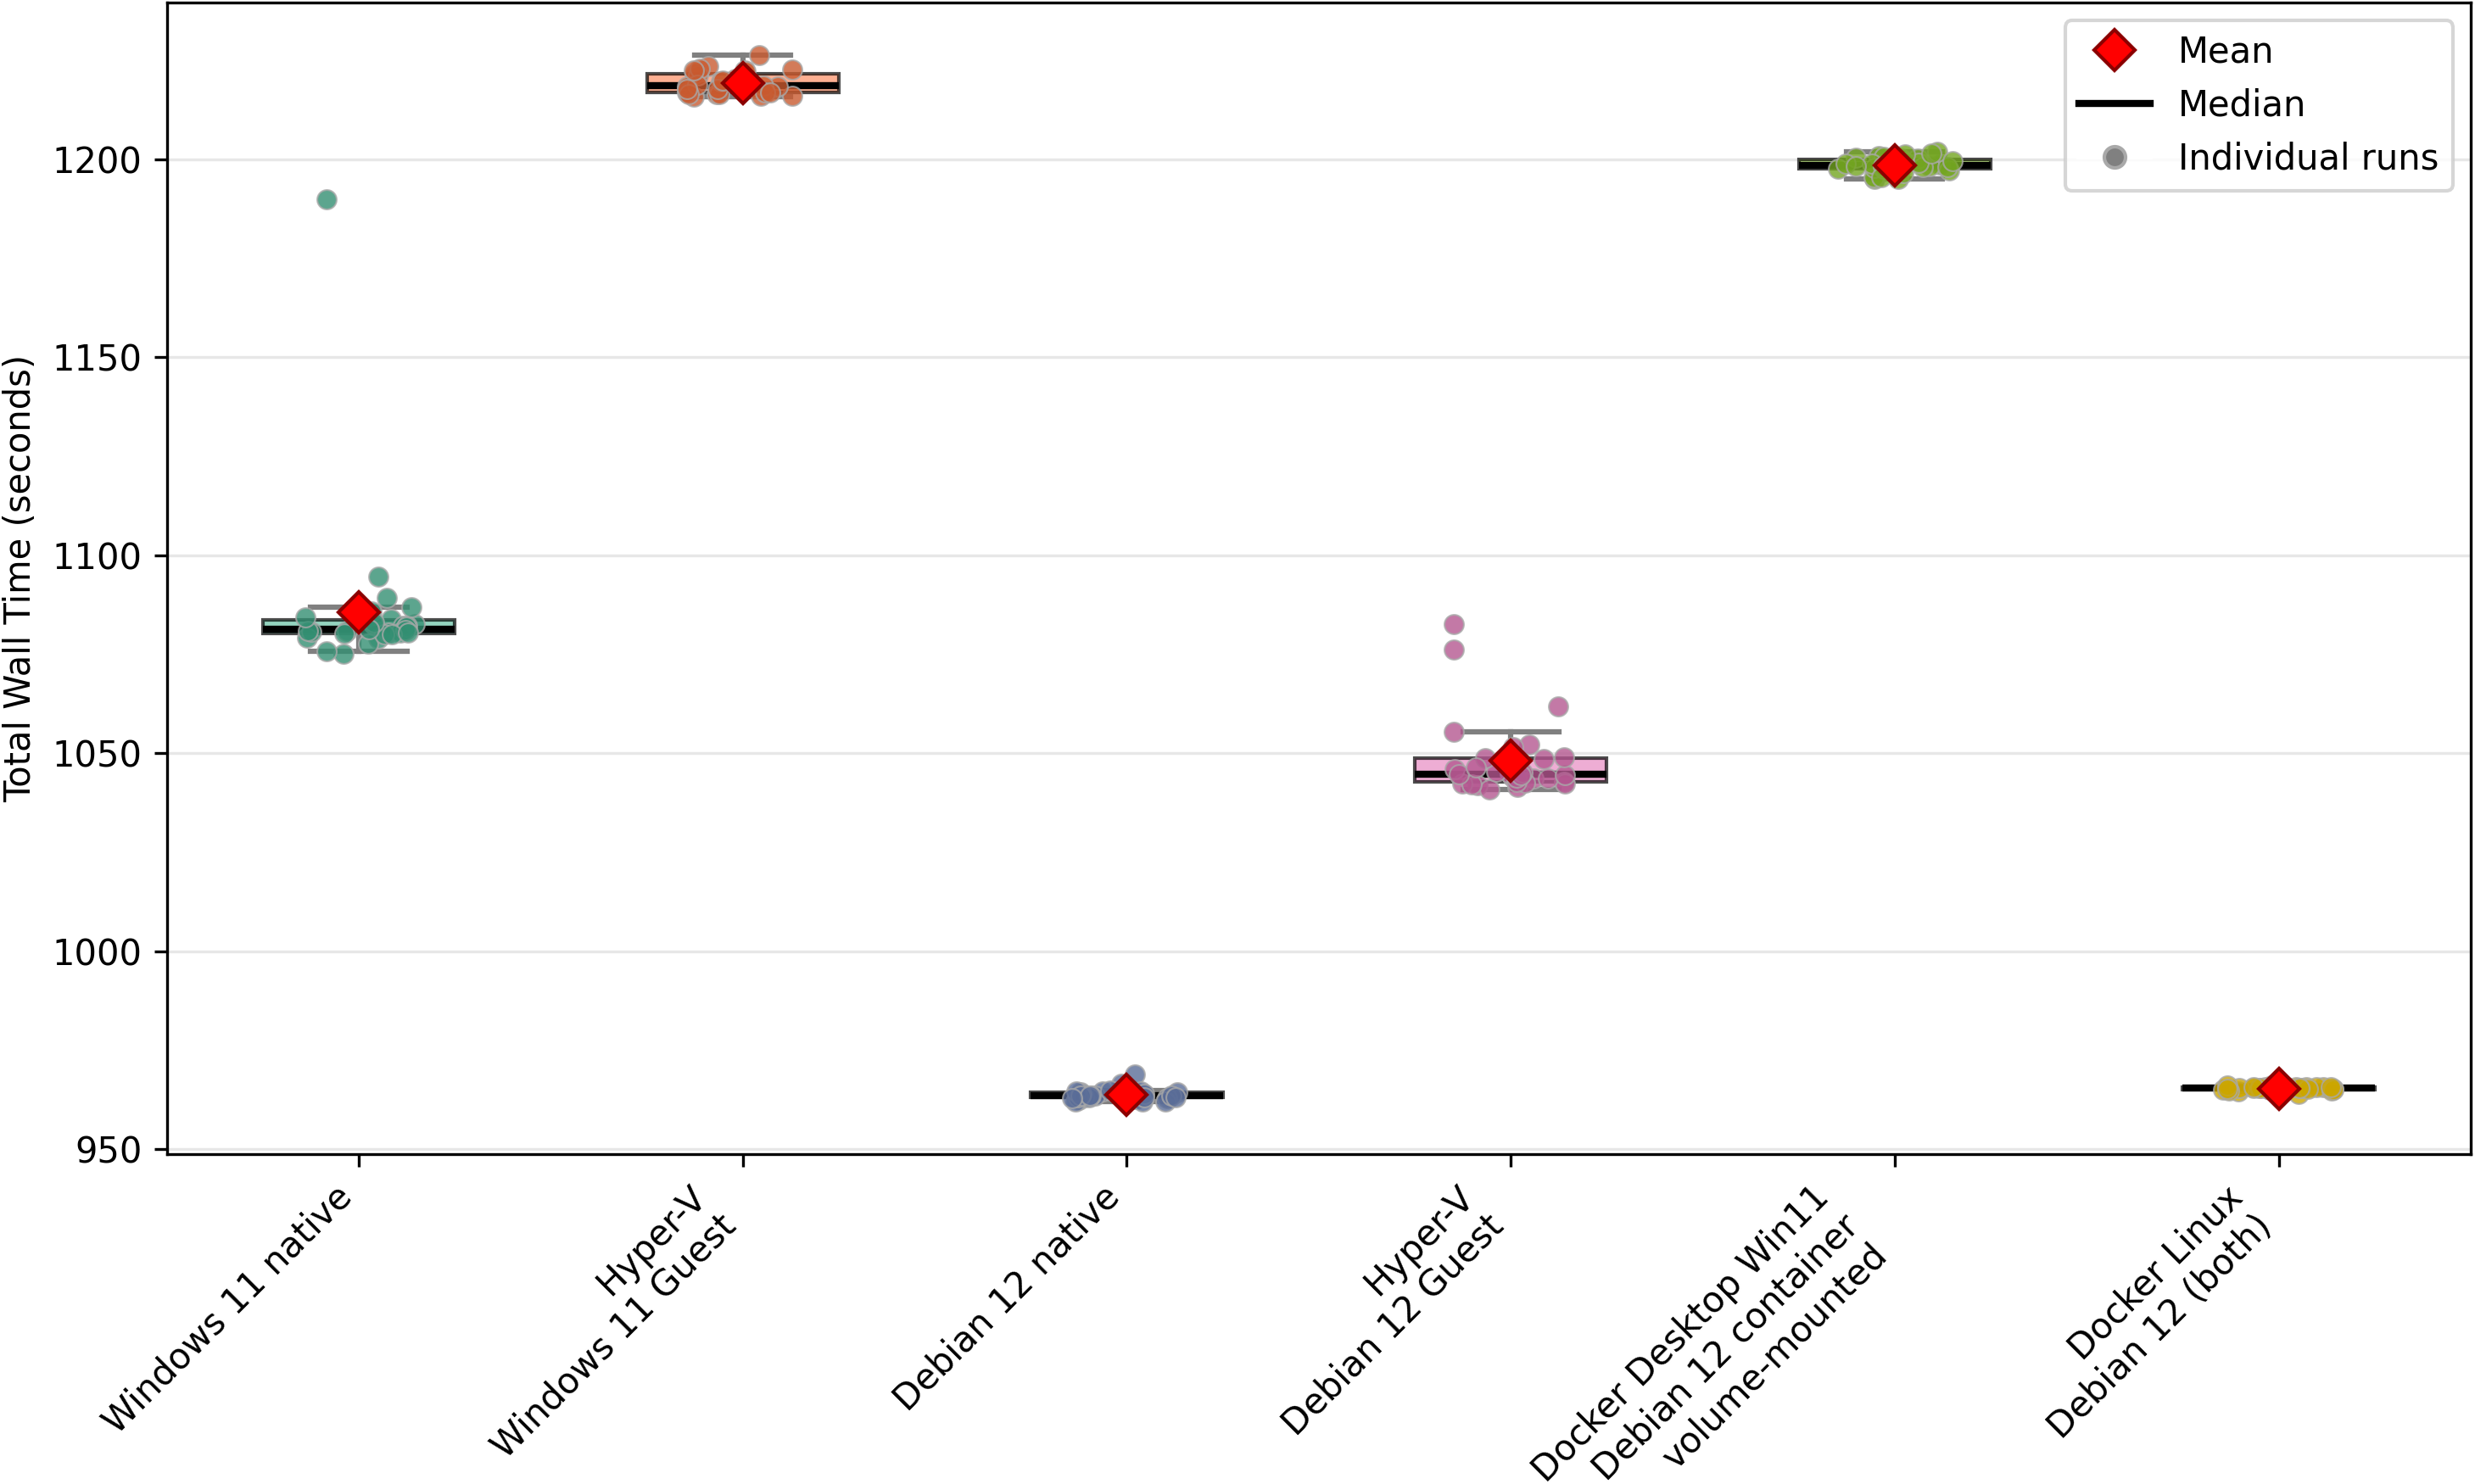
\includegraphics[width=\linewidth]{figures/scenario_2_boxplot_total_runtime.png}
    \caption{Total runtime distribution for complete development workflow (n=30)}
    \label{fig:total_runtime}
\end{figure}

Linux-based environments consistently outperform the Windows native baseline.
Debian native and Docker on Linux achieve nearly identical results (10.9\% and 10.7\% faster respectively), demonstrating that containerization imposes minimal overhead when host and container share the same kernel.
Even Hyper-V Debian Guest completes the workflow 3.4\% faster than Windows native despite virtualization overhead, indicating that Linux toolchains handle filesystem-intensive build operations more efficiently.

Windows-based environments show longer total runtimes, with hypervisor-based configurations incurring additional overhead.
Hyper-V Windows Guest (12.7\% slower) and Docker Desktop (10.8\% slower) accumulate latency from virtualization and WSL2 translation layers across both CPU-bound compilation and I/O-bound operations.

Docker Desktop on Windows presents an interesting trade-off: while the complete workflow takes 10.8\% longer than native Windows, individual I/O-bound operations show significant improvements---configuration runs 35.8\% faster and incremental builds complete 47.8--66.0\% faster.
This suggests faster iteration cycles for common development tasks despite the overall workflow overhead.

Consistency varies significantly across environments.
Debian native and Docker Linux maintain sub-second standard deviations (1.37s and 0.44s respectively) across the 16-minute workflow.
Docker Desktop shows 1.87-second variability, while Windows native exhibits 20.06 seconds of variance, reflecting accumulated inconsistency from I/O performance fluctuations.

\subsubsection{Excluded configuration: Docker Desktop with non-native bind mounts}
\label{subsec:excluded_bind_mounts}

Docker Desktop on Windows supports two methods for container source code access: bind mounts and named volumes.
Bind mounts expose host filesystem paths directly, while named volumes store data within Docker's managed storage layer.
On native Linux, bind mounts perform efficiently as container and host share the same filesystem layer.
On Windows, however, bind mounts require cross-filesystem translation between NTFS and the Linux container environment.
The preceding Docker Desktop benchmarks used volume-mounted source code; this section documents why bind mounts were excluded.

Initial testing revealed severe bind mount performance degradation compared to volume mounts, confirming findings by \citet{dockerDockerDesktopWSL2020,cncfDockerMacOSSlow2023}.
Due to the extreme penalty, only a single exploratory benchmark run was conducted; results should be interpreted as indicative rather than statistically robust.
Table~\ref{tab:bind_mount_comparison} and Figure~\ref{fig:bind_mount_build_comparison} present the comparison.

\begin{table}[ht]
    \centering
    \footnotesize
    \begin{tabular}{|l|r|r|r|r|r|}
        \hline
        \textbf{Operation} & \textbf{Volume Mount} & \textbf{Bind Mount} & \textbf{Overhead} & \textbf{CPU Vol.} & \textbf{CPU Bind} \\
        & \textbf{Median (s)} & \textbf{Time (s)} & & \textbf{Median (\%)}  & \textbf{(\%)} \\
        \hline
        CMake Configure & 23.56 & 226.81 & +862.5\% & 5.05 & 1.92 \\
        Clean Build & 1150.11 & 10530.60 & +815.6\% & 99.48 & 18.24 \\
        Installation & 16.09 & 892.97 & +5449.2\% & 3.34 & 1.33 \\
        \hline
    \end{tabular}
    \caption{Docker Desktop bind mount vs volume mount performance comparison (volume: n=30, bind: n=1)}
    \label{tab:bind_mount_comparison}
\end{table}

\begin{figure}[ht]
    \centering
    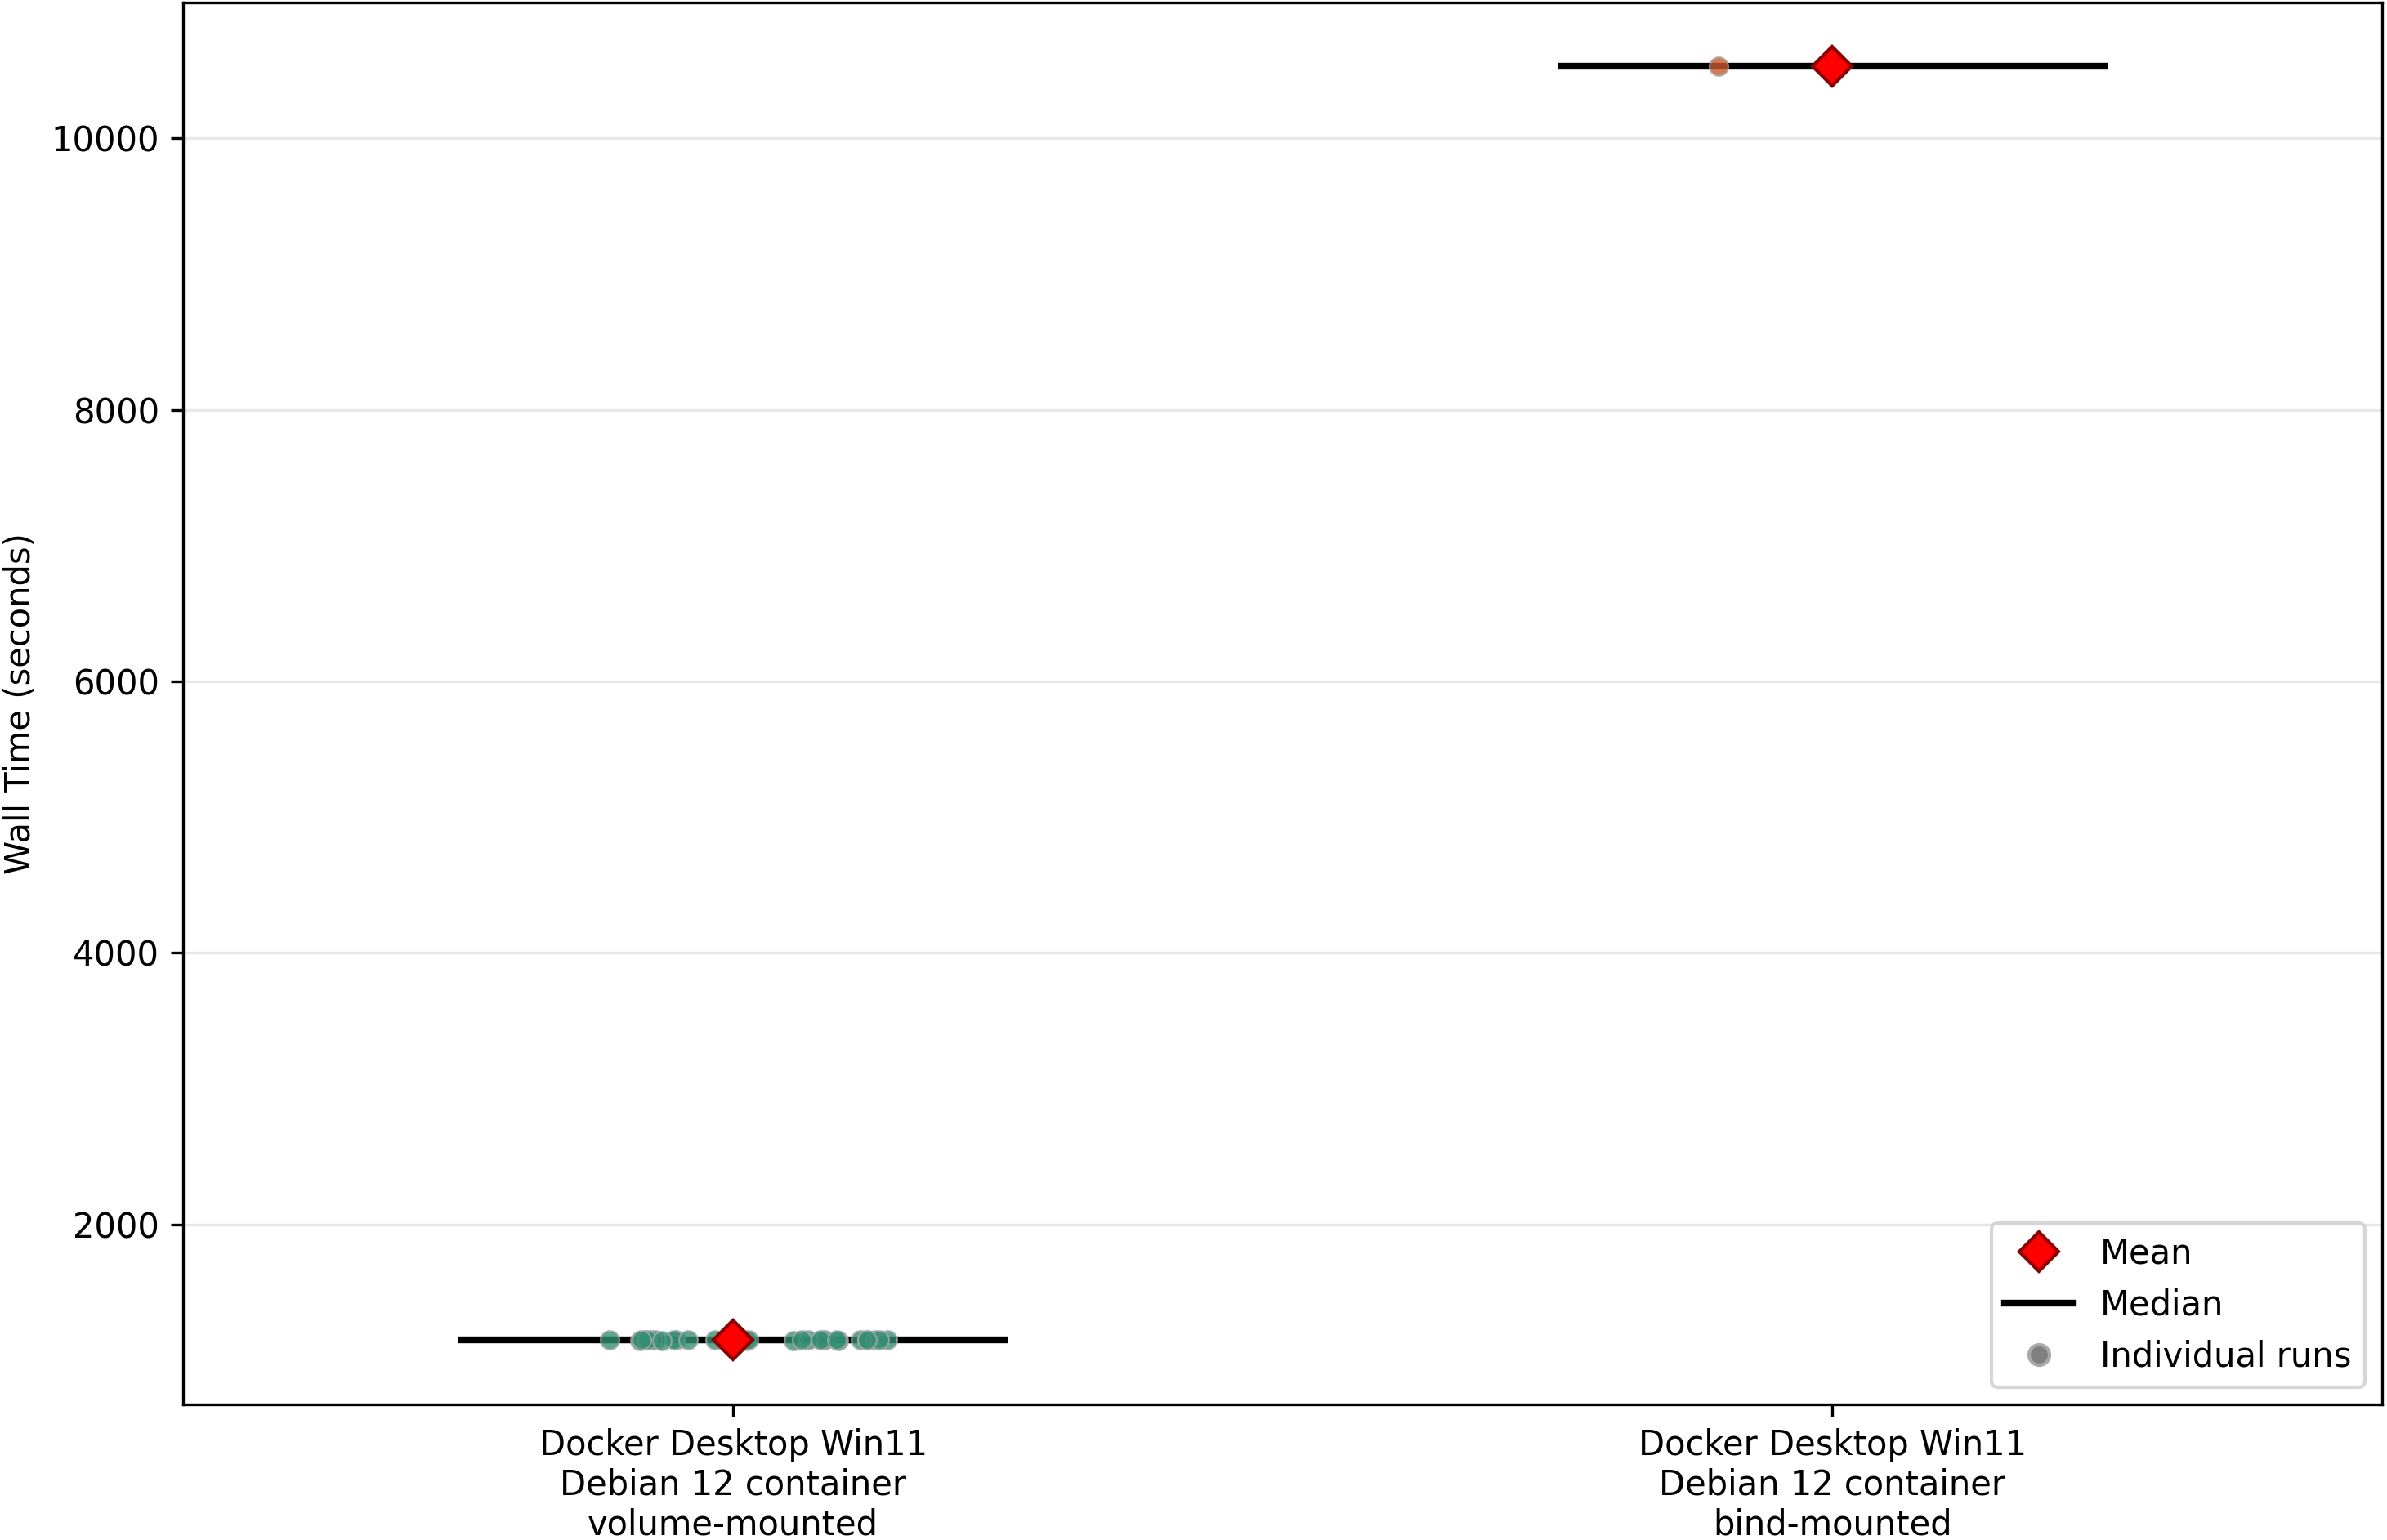
\includegraphics[width=\linewidth]{figures/scenario_2_dockerdesktop_bind_mount_boxplot_cmake_build_full_wall_time.png}
    \caption{Clean build wall time: volume mount distribution (n=30) vs bind mount single run}
    \label{fig:bind_mount_build_comparison}
\end{figure}

The bind mount configuration shows substantial performance degradation across all operations, with total workflow time increasing from approximately 20 minutes to over 3.2 hours (+879.5\% overhead).
The I/O-intensive installation workflow exhibits the most severe penalty at +5449.2\% overhead, while CPU-bound clean builds show +815.6\% overhead.

The performance penalty stems from the filesystem translation layer required to expose Windows NTFS paths to Linux containers through WSL2.
Each filesystem operation must traverse multiple abstraction layers: the Windows host filesystem, the WSL2 virtualization boundary, and Docker's storage driver.
Volume mounts avoid this overhead by storing data directly within the WSL2 Linux filesystem, eliminating cross-boundary translation for most operations.
CPU utilization during bind-mounted builds remains low (18.3\% mean compared to 99.6\% for volume mounts), indicating that the system spends most time waiting for filesystem operations rather than performing compilation work.

This finding has practical implications for containerized development workflows on Windows: developers must use volume-mounted source code or accept order-of-magnitude performance penalties.
The volume mount approach requires copying source code into Docker volumes or cloning it directly there rather than accessing the Windows filesystem, adding workflow complexity but delivering substantially better performance.
The benchmarks in this evaluation exclusively use volume mounts for Docker Desktop on Windows to represent the practical, performance-optimized containerized workflow.

\subsection{Unit test execution}
\label{subsec:unittest_execution}

Unit test execution represents a critical component of development workflows, providing rapid feedback on code correctness during iterative development.
This subsection documents the unit test execution benchmarks and their limitations within the evaluated legacy codebase.

\subsubsection{Test suite characteristics and limitations}

The unit test suite accumulated over decades of development without consistent cross-platform validation.
During benchmark preparation, the test suite demonstrated platform-dependent behavior: while tests executed reliably on Windows environments, Linux-based environments exhibited unexplained slowdowns, and Docker Desktop on Windows failed to complete within reasonable timeouts.

These failures prevented inclusion of unit test execution in the standard benchmark suite (Sections \ref{subsec:cmake_configure}--\ref{subsec:total_runtime_standard}), as inconsistent pass/fail rates would confound performance measurements with correctness variations.
The test instability reflects a common challenge in legacy software: accumulated technical debt in test infrastructure that reduces confidence in automated testing outcomes.

Despite these limitations, unit test execution remains relevant for evaluating environment performance characteristics.
The following sections present results from test execution benchmarks conducted with acknowledgement of the underlying test reliability issues, focusing on execution time rather than test outcomes.

\subsubsection{Sequential test execution performance}

Sequential test execution runs each test case serially, representing the most straightforward but slowest approach to test suite execution.
This baseline establishes the unoptimized test execution performance for comparison with parallel execution strategies.
A timeout of 1200 seconds was configured to prevent indefinite execution.

\begin{table}[ht]
    \centering
    \footnotesize
    \begin{tabular}{|l|r|r|r|r|r|}
        \hline
        \textbf{Environment} & \textbf{Mean (s)} & \textbf{Median (s)} & \textbf{vs Baseline} & \textbf{Std Dev} & \textbf{Max (s)} \\
        \hline
        Win11 native & 415.55 & 415.20 & baseline & 8.56 & 437.36 \\
        Hyper-V Win11 & 423.12 & 423.19 & +1.9\% & 3.50 & 429.12 \\
        Debian native & 815.09 & 814.62 & +96.2\% & 3.83 & 826.06 \\
        Hyper-V Debian & 862.18 & 854.20 & +105.7\% & 16.50 & 909.94 \\
        Docker Desktop & 1201.01 & 1200.19 & +189.1\% & 2.77 & 1215.05 \\
        Docker Linux & 811.44 & 810.51 & +95.2\% & 5.37 & 822.17 \\
        \hline
    \end{tabular}
    \caption{Sequential unit test execution performance (n=30)}
    \label{tab:unit_tests_sequential_s2}
\end{table}

\begin{figure}[ht]
    \centering
    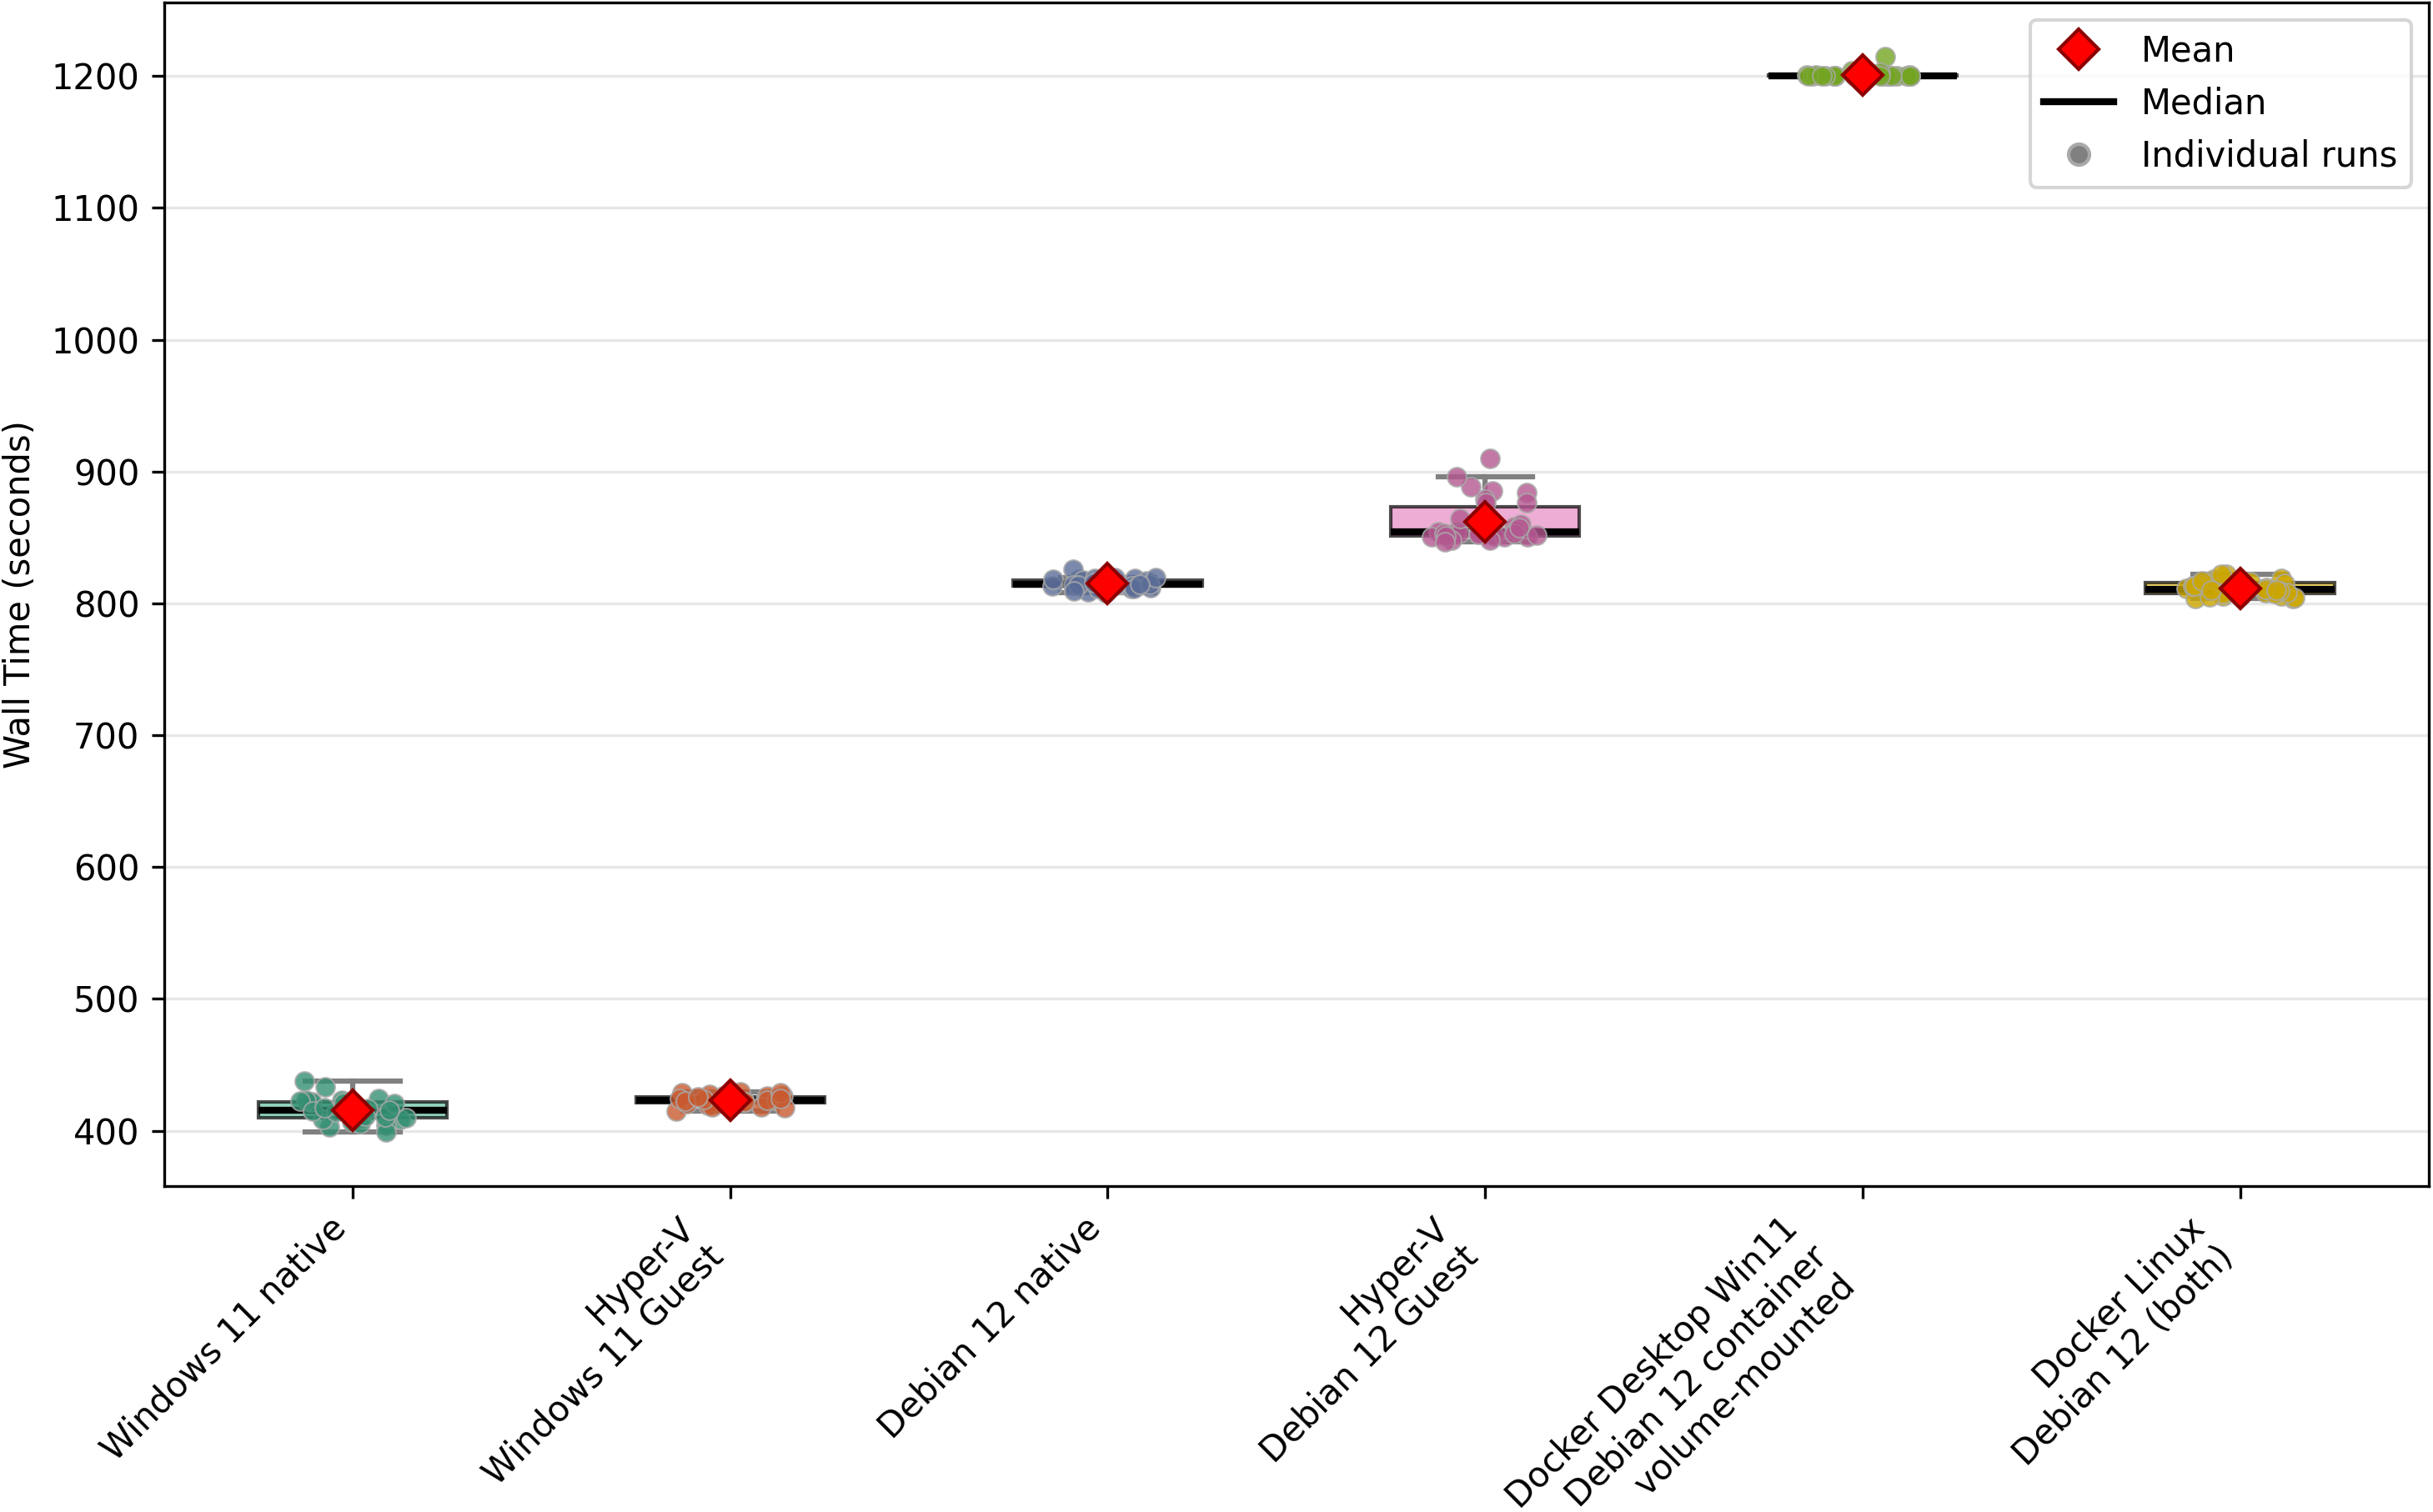
\includegraphics[width=\linewidth]{figures/scenario_2_unittests_boxplot_unit_tests_wall_time.png}
    \caption{Sequential unit test execution wall time distribution across environments (n=30)}
    \label{fig:unit_tests_sequential_wall_time}
\end{figure}

The results show an inversion of the performance patterns observed in build benchmarks: Windows environments outperform Linux-based environments for unit test execution.
Windows native completes the test suite in 415.20 seconds median (approximately 6.9 minutes), with Hyper-V Windows adding minimal overhead (+1.9\%).

All Linux-based environments require approximately twice the Windows execution time: Debian native at 814.62 seconds (+96.2\%), Docker on Linux at 810.51 seconds (+95.2\%), and Hyper-V Debian at 854.20 seconds (+105.7\%).
The similar performance between native and containerized Linux confirms that the slowdown originates from the test suite's interaction with Linux rather than deployment overhead.

Docker Desktop failed to complete within the 1200-second timeout on any run, with the median of 1200.19 seconds and tight clustering (standard deviation 2.77s) indicating consistent timeout termination.
The root cause of this cross-platform performance disparity was not investigated within the scope of this evaluation.

\subsubsection{Parallel test execution performance}

Parallel test execution leverages CTest's ability to run multiple test cases concurrently, reducing total test suite execution time on multi-core systems.
Given Docker Desktop's inability to complete sequential test execution within the timeout, parallel benchmarks were conducted only on Windows native and Debian native environments, with a parallelization factor of 20 concurrent tests and a reduced timeout of 240 seconds.

\begin{table}[htbp]
    \centering
    \footnotesize
    \begin{tabular}{|l|l|r|r|r|r|}
        \hline
        \textbf{Platform} & \textbf{Mode} & \textbf{Mean (s)} & \textbf{Median (s)} & \textbf{Std Dev} & \textbf{Median Reduction} \\
        \hline
        \multirow{2}{*}{Win11 native} & Sequential & 415.55 & 415.20 & 8.56 & --- \\
        & Parallel (20) & 175.76 & 175.98 & 3.57 & $-$57.6\% \\
        \hline
        \multirow{2}{*}{Debian native} & Sequential & 815.09 & 814.62 & 3.83 & --- \\
        & Parallel (20) & 119.13 & 92.06 & 63.74 & $-$88.7\% \\
        \hline
    \end{tabular}
    \caption{Parallel unit test execution: sequential vs parallel comparison (n=30)}
    \label{tab:unit_tests_parallel_s2}
\end{table}

\begin{table}[htbp]
    \centering
    \footnotesize
    \begin{tabular}{|l|l|r|r|}
        \hline
        \textbf{Platform} & \textbf{Mode} & \textbf{CPU $\Delta$ Mean} & \textbf{Mem $\Delta$ Peak} \\
        & & \textbf{Median (\%)} & \textbf{Median (MB)} \\
        \hline
        \multirow{2}{*}{Win11 native} & Sequential & $-$0.96 & $-$102.83 \\
        & Parallel (20) & 5.41 & 3775.04 \\
        \hline
        \multirow{2}{*}{Debian native} & Sequential & 1.48 & 595.10 \\
        & Parallel (20) & 5.49 & 845.95 \\
        \hline
    \end{tabular}
    \caption{Parallel unit test execution: resource consumption (n=30)}
    \label{tab:unit_tests_parallel_resources_s2}
\end{table}

\begin{figure}[htbp]
    \centering
    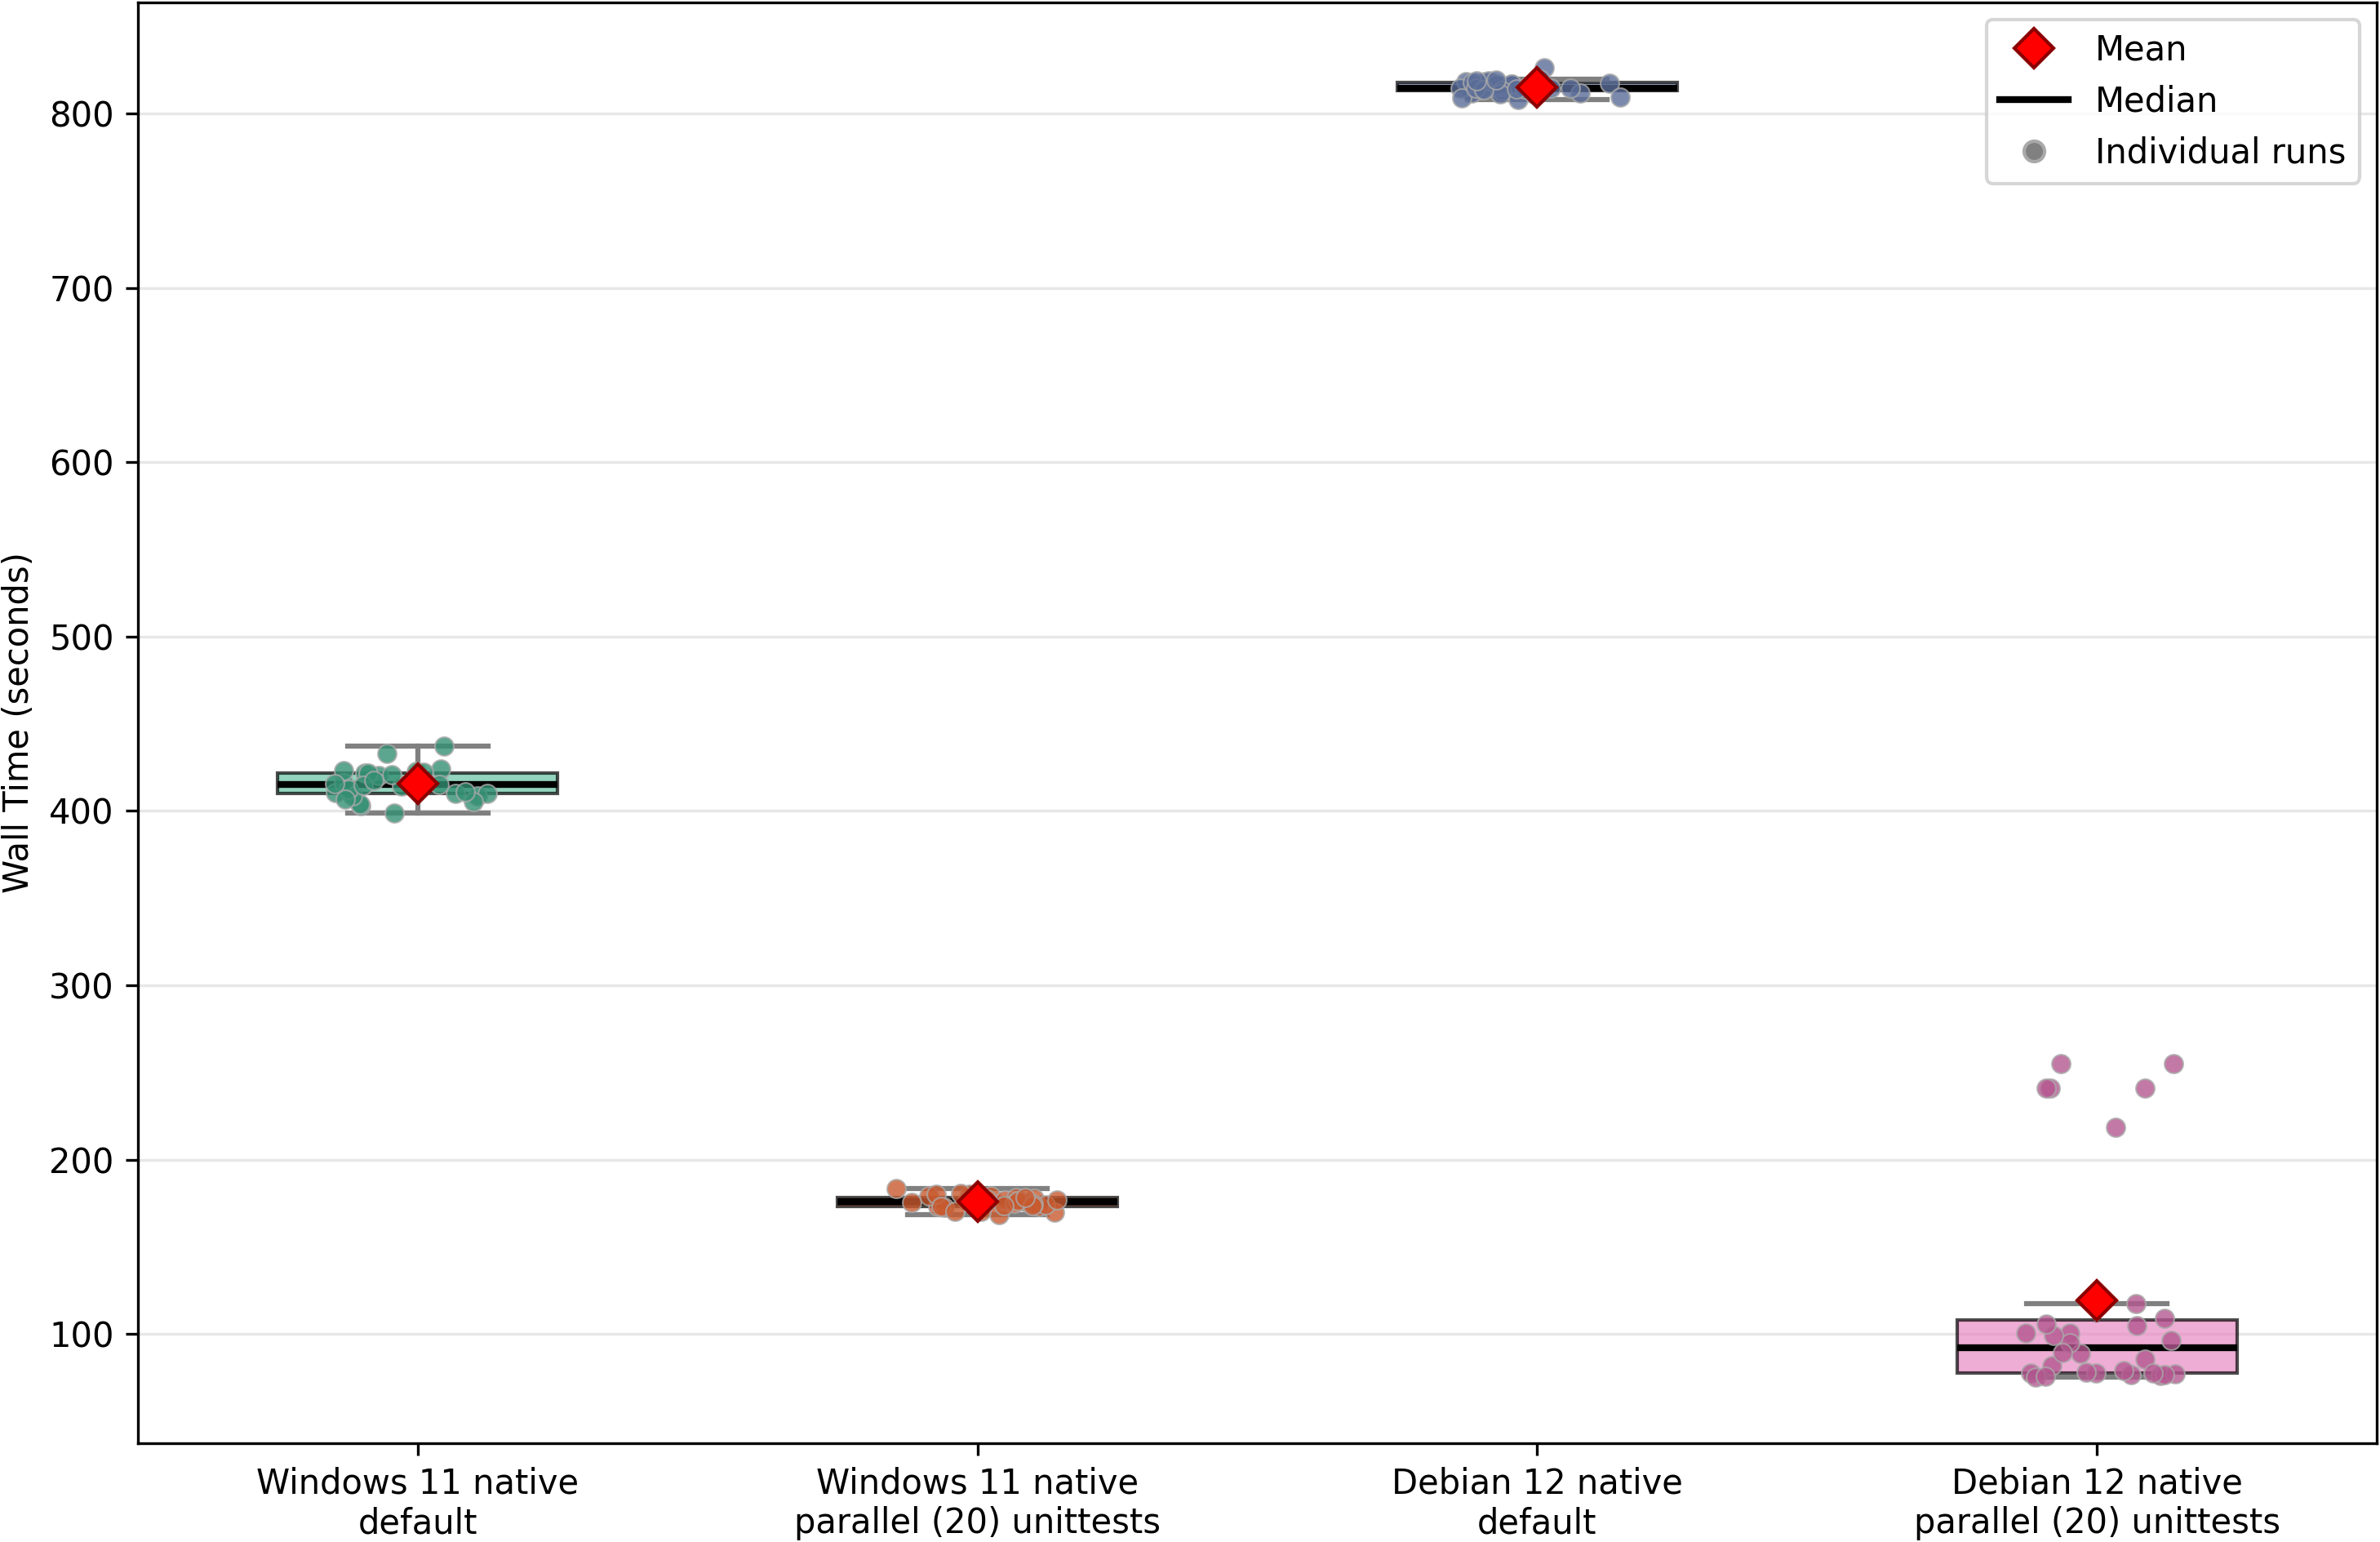
\includegraphics[width=\linewidth]{figures/scenario_2_unittests_parallel_boxplot_unit_tests_wall_time.png}
    \caption{Parallel vs sequential unit test execution wall time distribution (n=30)}
    \label{fig:unit_tests_parallel_wall_time}
\end{figure}

Parallel execution improves test suite performance on both platforms.
Windows native achieves a 57.6\% reduction in median execution time (175.98s vs 415.20s), yielding a 2.36$\times$ speedup from 20 parallel jobs.
Debian native shows an 88.7\% reduction in median execution time (92.06s vs 814.62s), though with high variability: the standard deviation of 63.74 seconds and the gap between mean (119.13s) and median (92.06s) indicate that some runs approached the 240-second timeout while others completed in under 80 seconds.

While sequential Linux execution was nearly twice as slow as Windows, parallel Linux execution (median 92.06s) outperforms parallel Windows execution (median 175.98s) by 47.7\% when runs complete without timeout.
This reversal suggests that the sequential slowdown on Linux may stem from test ordering or synchronization issues that parallel execution circumvents.

Resource consumption increases with parallelization.
CPU delta rises from near-idle or slightly negative baseline levels to approximately 5.4--5.5\% on both platforms.
The negative delta values for Windows sequential execution ($-$0.96\% CPU, $-$102.83 MB memory) indicate that system resource usage decreased slightly during test execution compared to the pre-benchmark baseline, likely due to background processes completing or system services releasing resources during the measurement period.
Peak memory delta increases substantially with parallelization: Windows parallel execution requires 3.8 GB additional memory, while Debian parallel execution shows a median increase of 845 MB with outliers reaching several gigabytes.

\subsection{Optimized workflow with compiler caching}
\label{subsec:optimized_workflow}

This subsection evaluates the performance impact of sccache, a distributed compiler cache, across the evaluated environments.
Sccache intercepts compiler invocations and caches compilation results based on input file hashes, compiler flags, and other deterministic factors.
Subsequent compilations with identical inputs retrieve cached results instead of re-executing the compiler.
Cache effectiveness depends on the stability of compilation inputs: changes to headers, compiler versions, or build flags invalidate cached results \citep{mozillaSccacheSharedCompilation2025}.

For this evaluation, only cache-warm full builds were measured to demonstrate the maximum achievable speedup; other optimized workflow benchmarks (incremental builds with caching, cache-cold scenarios) were out of scope.
Cache-warm builds retrieve pre-computed results for all compilation units, representing the ideal case for developers performing repeated builds during iterative development.

\begin{table}[htbp]
    \centering
    \footnotesize
    \begin{tabular}{|l|r|r|r|r|r|}
        \hline
        \textbf{Environment} & \textbf{Wall Time} & \textbf{vs Win11} & \textbf{CPU $\Delta$ Mean} & \textbf{Mem $\Delta$ Peak} & \textbf{Host Peak Mem} \\
        & \textbf{Median (s)} & \textbf{Native} & \textbf{Median (\%)} & \textbf{Median (MB)} & \textbf{Median (MB)} \\
        \hline
        Win11 native & 224.47 & baseline & 99.02 & 8805.44 & --- \\
        Hyper-V Win11 & 254.72 & +13.5\% & 98.53 & 8086.34 & 11493.00 \\
        Debian native & 37.90 & $-$83.1\% & 79.12 & 3530.46 & --- \\
        Hyper-V Debian & 40.53 & $-$81.9\% & 76.89 & 3344.21 & 20480 \\
        Docker Desktop & 42.26 & $-$81.2\% & 83.29 & 4122.80 & 19960.06 \\
        Docker Linux & 37.83 & $-$83.1\% & 79.85 & 3432.59 & --- \\
        \hline
    \end{tabular}
    \caption{Cache-warm clean build performance with sccache (n=30)}
    \label{tab:cmake_build_full_cached_s2}
\end{table}

\begin{figure}[htbp]
    \centering
    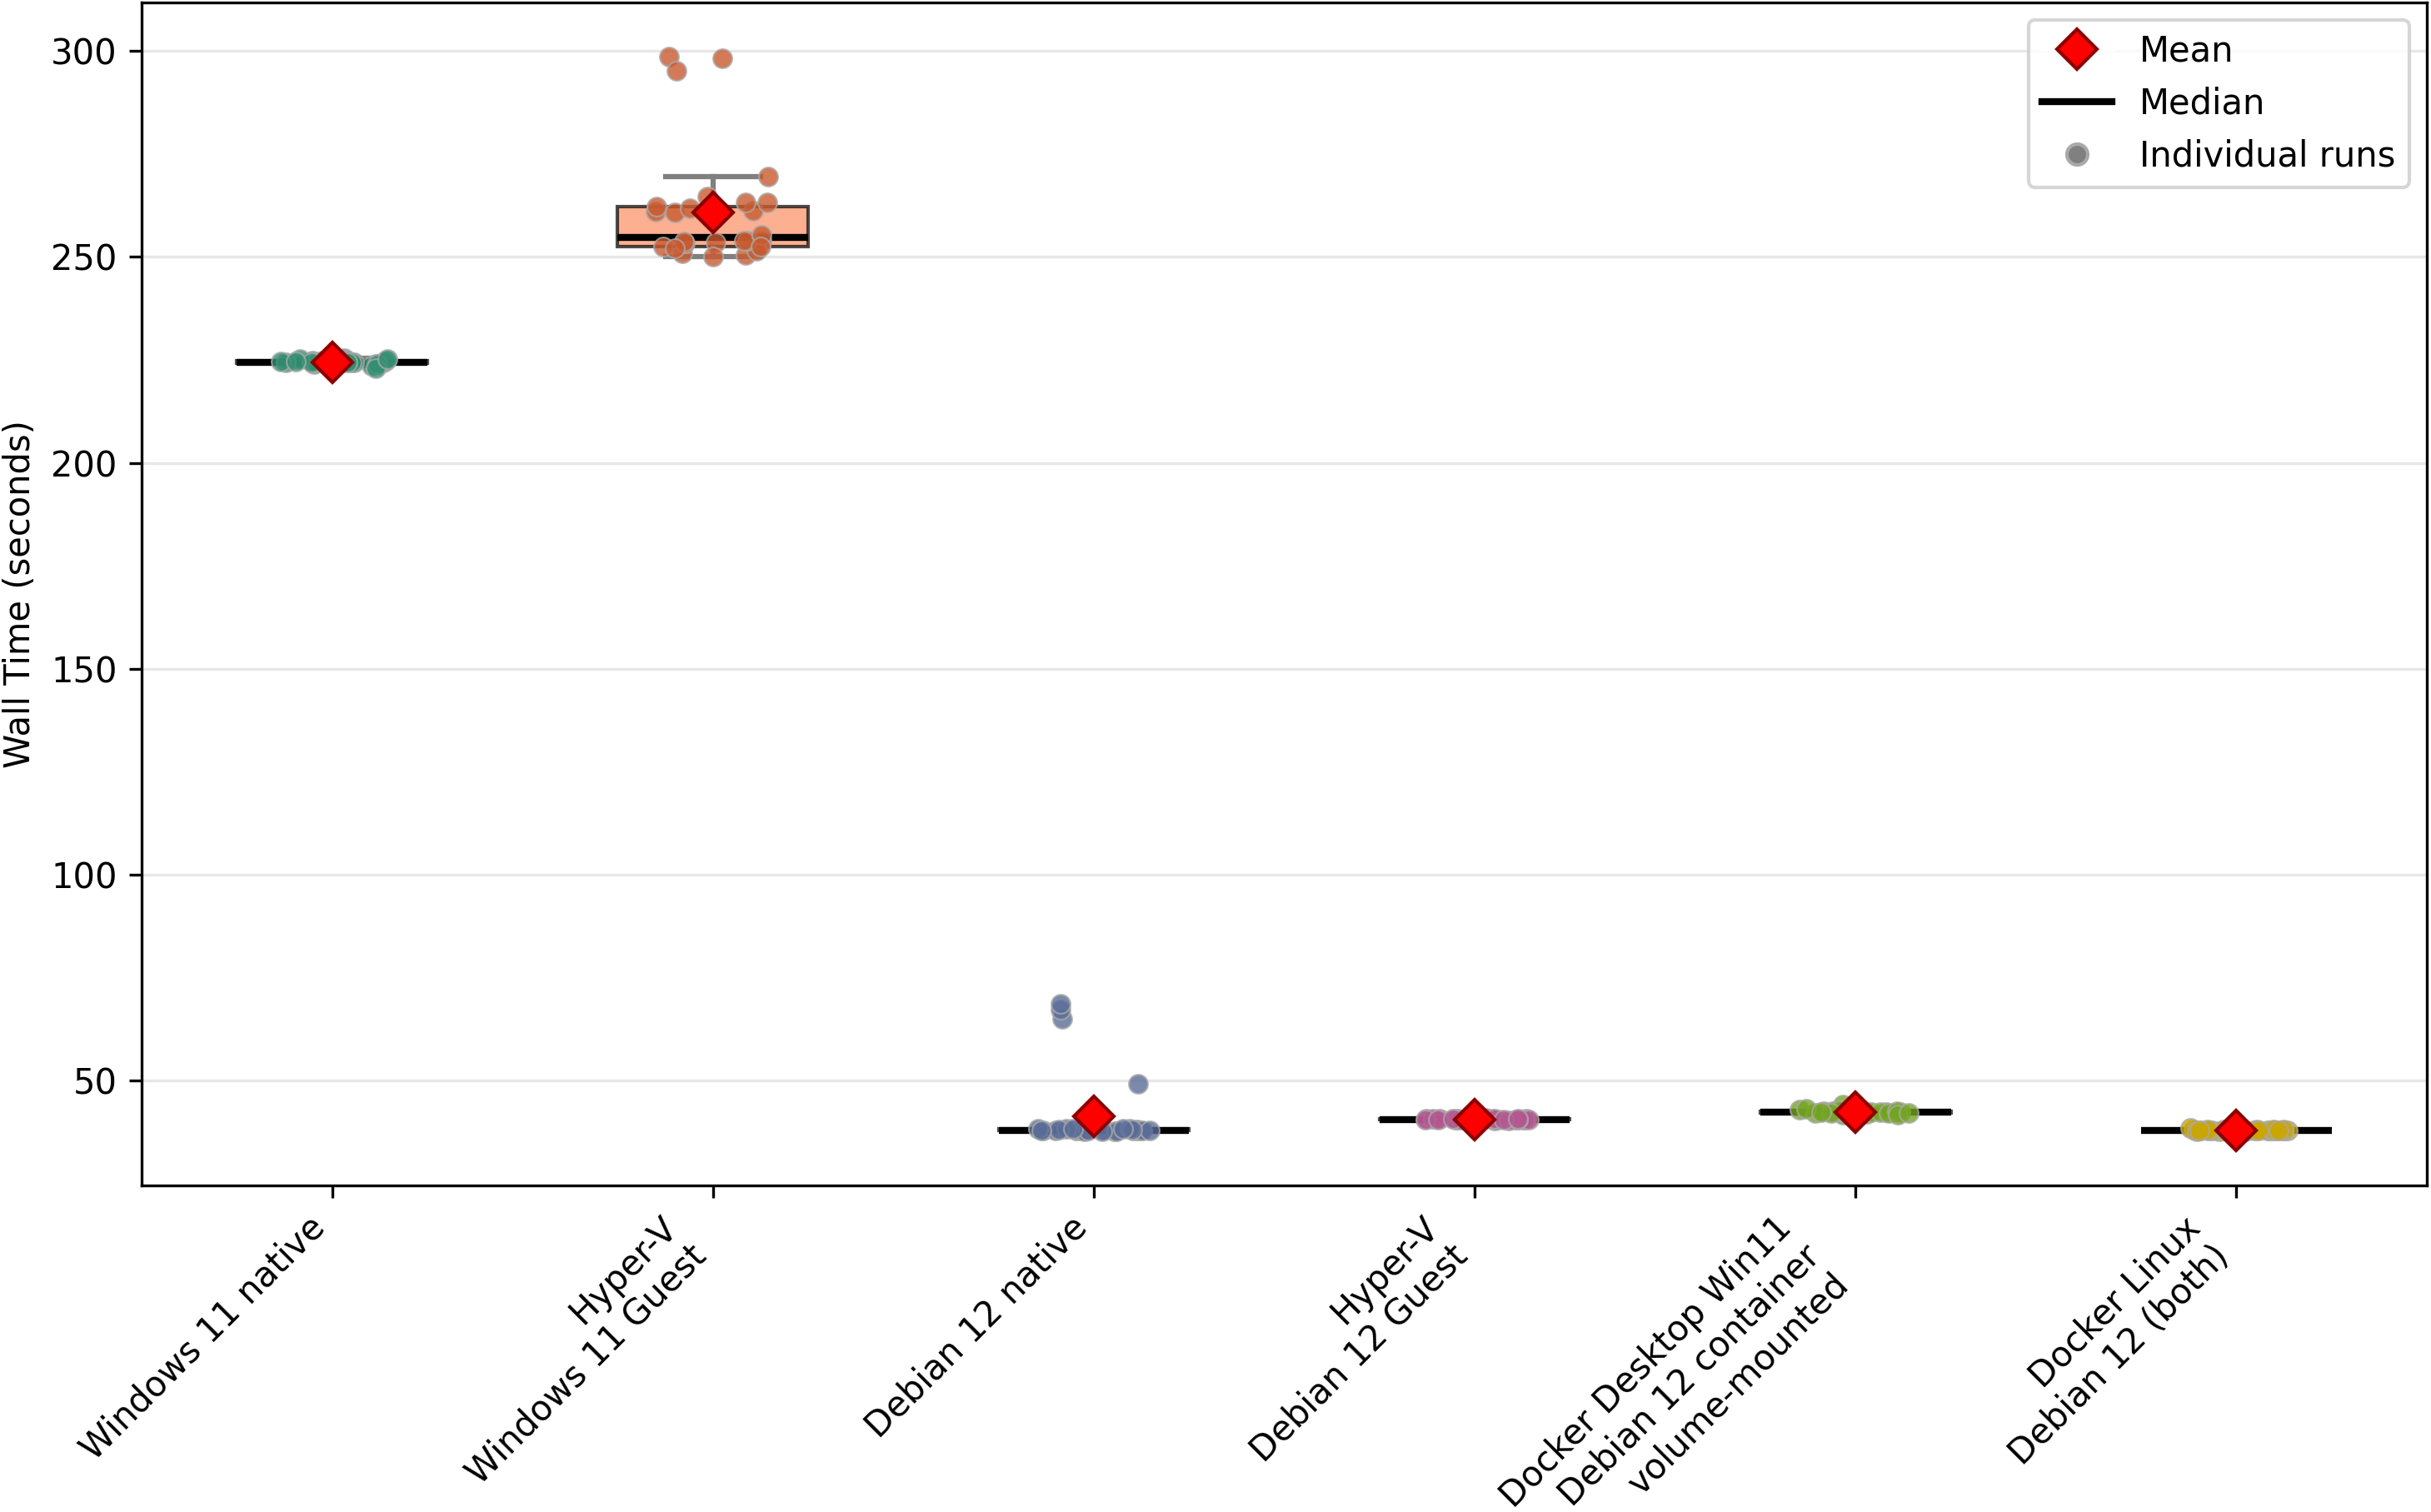
\includegraphics[width=\linewidth]{figures/scenario_2_cached_boxplot_cmake_build_full_wall_time.png}
    \caption{Cache-warm clean build wall time distribution across environments (n=30)}
    \label{fig:cmake_build_full_cached_wall_time}
\end{figure}

Table~\ref{tab:cmake_build_full_cached_s2} and Figure~\ref{fig:cmake_build_full_cached_wall_time} present cache-warm build performance.
Linux-based environments show an 81--83\% reduction in build time compared to the Windows native baseline, completing in 37.83--42.26 seconds.
Windows native requires 224.47 seconds, while Hyper-V Windows Guest shows +13.5\% overhead at 254.72 seconds.
This contrasts with uncached results (Section \ref{subsec:clean_build}) where all environments showed similar absolute performance within a 24\% range.

Host-side memory for hypervisor-based environments ranges from 11.2--20.0 GB, including guest OS overhead.

Table~\ref{tab:cmake_build_full_cached_comparison} compares uncached and cache-warm build performance.

\begin{table}[htbp]
    \centering
    \footnotesize
    \begin{tabular}{|l|r|r|r|r|}
        \hline
        \textbf{Environment} & \textbf{Uncached} & \textbf{Cache-warm} & \textbf{Speedup} & \textbf{vs Uncached} \\
        & \textbf{Median (s)} & \textbf{Median (s)} & \textbf{Factor} & \textbf{Win11 Native} \\
        \hline
        Win11 native & 1003.89 & 224.47 & 4.5$\times$ & $-$77.6\% \\
        Hyper-V Win11 & 1106.19 & 254.72 & 4.3$\times$ & $-$74.6\% \\
        Debian native & 930.17 & 37.90 & 24.5$\times$ & $-$96.2\% \\
        Hyper-V Debian & 1000.40 & 40.53 & 24.7$\times$ & $-$96.0\% \\
        Docker Desktop & 1150.11 & 42.26 & 27.2$\times$ & $-$95.8\% \\
        Docker Linux & 931.30 & 37.83 & 24.6$\times$ & $-$96.2\% \\
        \hline
    \end{tabular}
    \caption{Clean build performance: uncached vs cache-warm comparison}
    \label{tab:cmake_build_full_cached_comparison}
\end{table}

Linux-based environments achieve 24--27$\times$ speedup factors, reducing build times from approximately 15--19 minutes to under 45 seconds.
Windows environments show 4--5$\times$ improvements, reducing builds from 17--18 minutes to approximately 3.7--4.4 minutes.
Compared to uncached Windows native builds, Linux-based environments with caching achieve approximately 96\% reduction.

CPU utilization during cache-warm builds shows 77--83\% on Linux environments compared to 98--99\% on Windows.
The lower Linux CPU utilization reflects reduced computational work when retrieving cached results.
Peak memory consumption on Linux environments shows 3.3--4.1 GB delta versus 8.3--8.8 GB on Windows environments; uncached Linux builds showed 9.5--9.7 GB peak delta.

Regarding consistency, Docker Linux shows the tightest clustering with standard deviation of 0.13 seconds, while Windows native maintains 0.52 seconds standard deviation.
Debian native shows a standard deviation of 8.96 seconds, with occasional outliers reaching 68.50 seconds (compared to median 37.90s).

\subsection{Cumulative optimization impact}

This subsection compares unoptimized Windows native execution (sequential tests, no compiler caching) against optimized configurations with sccache and parallel test execution (20 concurrent tests) across Windows native, Docker Desktop, and Docker Linux environments.
Figure~\ref{fig:optimization_compare_total_runtime} and Table~\ref{tab:optimization_compare_total_runtime} present the total runtime comparison.

\begin{figure}[htbp]
    \centering
    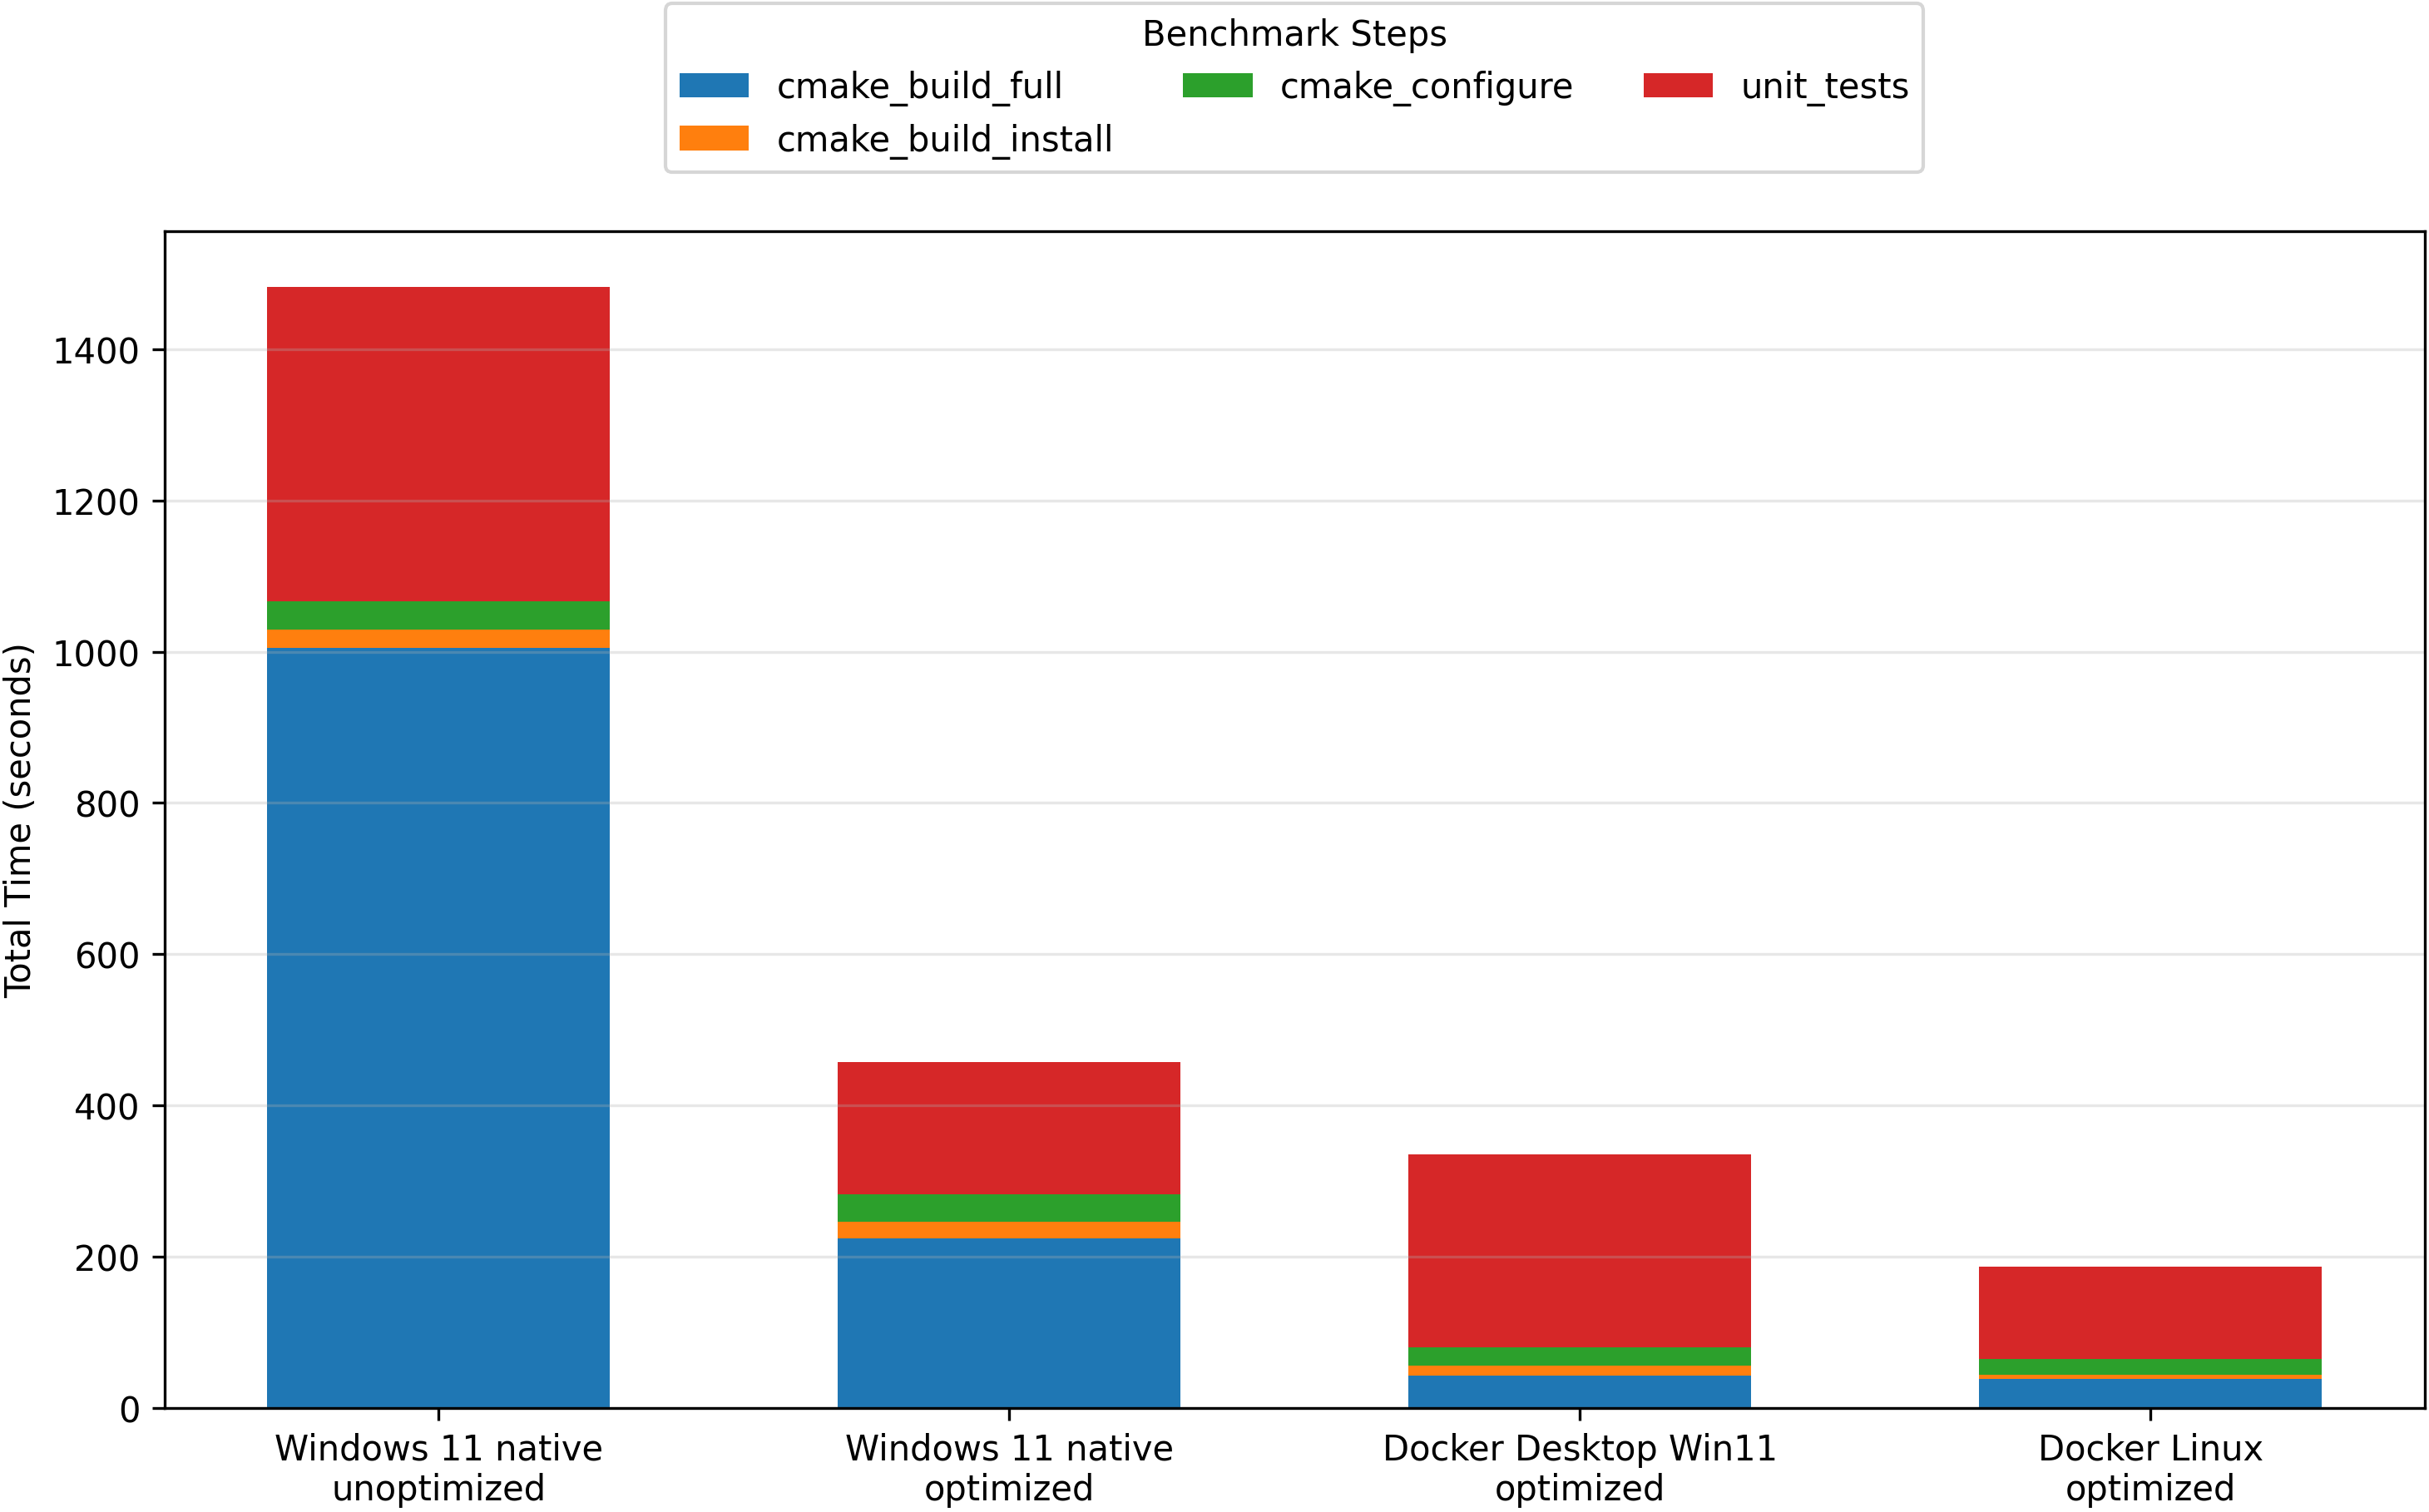
\includegraphics[width=\linewidth]{figures/scenario_2_optimization_compare_wall_time.png}
    \caption{Total runtime comparison: unoptimized vs optimized workflows (n=30)}
    \label{fig:optimization_compare_total_runtime}
\end{figure}

\begin{table}[htbp]
    \centering
    \footnotesize
    \begin{tabular}{|l|r|r|r|}
        \hline
        \textbf{Environment} & \textbf{Wall Time} & \textbf{vs Unoptimized} & \textbf{vs Optimized} \\
        & \textbf{Median (s)} & \textbf{Baseline} & \textbf{Win11 native} \\
        \hline
        Win11 native (unoptimized) & 1478.80 & baseline & --- \\
        Win11 native (optimized) & 457.12 & $-$69.1\% & baseline \\
        Docker Desktop (optimized) & 335.09 & $-$77.3\% & $-$26.7\% \\
        Docker Linux (optimized) & 164.44 & $-$88.9\% & $-$64.0\% \\
        \hline
    \end{tabular}
    \caption{Total runtime comparison: unoptimized vs optimized workflows (n=30)}
    \label{tab:optimization_compare_total_runtime}
\end{table}

Optimization techniques reduce the Windows native workflow from 1478.80 seconds (24.6 minutes) to 457.12 seconds (7.6 minutes), a 69.1\% reduction.
Docker Desktop achieves 335.09 seconds (5.6 minutes, 77.3\% reduction), while Docker Linux reaches 164.44 seconds (2.7 minutes, 88.9\% reduction).

\begin{table}[htbp]
    \centering
    \footnotesize
    \begin{tabular}{|l|r|r|r|r|}
        \hline
        \textbf{Operation} & \textbf{Win11 native} & \textbf{Win11 native} & \textbf{Docker Desktop} & \textbf{Docker Linux} \\
        & \textbf{(unoptimized)} & \textbf{(optimized)} & \textbf{(optimized)} & \textbf{(optimized)} \\
        & \textbf{Median (s)} & \textbf{Median (s)} & \textbf{Median (s)} & \textbf{Median (s)} \\
        \hline
        CMake Configure & 36.69 & 36.05 & 24.51 & 20.98 \\
        Clean Build & 1003.89 & 224.47 & 42.26 & 37.83 \\
        Installation & 21.80 & 21.26 & 13.28 & 5.55 \\
        Unit Tests & 415.20 & 175.98 & 255.13 & 100.16 \\
        \hline
        \textbf{Total} & \textbf{1478.80} & \textbf{457.12} & \textbf{335.09} & \textbf{164.44} \\
        \hline
    \end{tabular}

    \smallskip
    \footnotesize
    \textit{Note: Total represents median of per-run total wall time, not sum of operation medians.}
    \caption{Per-operation breakdown: unoptimized vs optimized workflows (n=30)}
    \label{tab:optimization_compare_breakdown}
\end{table}

Table~\ref{tab:optimization_compare_breakdown} shows that clean builds contribute the largest absolute time reduction: from 1003.89 seconds unoptimized to 224.47 seconds with caching on Windows native (77.6\%), and to 42.26 seconds on Docker Desktop and 37.83 seconds on Docker Linux (95.8\% and 96.2\% reductions respectively).

Unit test results show varying effectiveness.
Windows native parallel execution achieves 175.98 seconds (57.6\% reduction from sequential baseline).
Docker Desktop requires 255.13 seconds with parallel execution---this result reflects the test suite reliability issues documented in Section~\ref{subsec:unittest_execution}, where Docker Desktop consistently approached or exceeded timeouts even with parallelization, preventing the expected performance improvements.
Docker Linux achieves 100.16 seconds median (75.9\% reduction), though with high variance due to the same underlying test instability.

Configuration and installation show consistent improvements: CMake configuration reduces from 36.69 to 20.98 seconds (primarily environment-dependent), while installation decreases from 21.80 to 5.55 seconds on Docker Linux.
The combination of compiler caching, parallel testing, and containerized Linux environments produces the largest cumulative workflow time reduction.

\section{Summary}

This chapter presented empirical measurements comparing development workflow performance across native, containerized, and virtualized environments through two complementary scenarios.
All measurements were conducted using the implemented prototype described in Chapter~\ref{ch:prototype_architecture}, demonstrating the practical reproducibility benefits: after completing the initial environment setup, all scenario 2 benchmarks could be executed with identical commands across all evaluated platforms.

The first scenario examined toolchain switching performance, measuring the time required to change development environments.
Native Windows toolchain switching via Visual Studio reinstallation required approximately 12.9 minutes, establishing the baseline.
Containerized approaches reduced this considerably: native Linux containers completed switching in 37.5 seconds (95.1\% improvement), while Docker Desktop on Windows achieved 1.68 minutes (87.0\% improvement).
Hyper-V virtualization fell between these at 3.6 minutes (71.8\% improvement).
The results indicate that container-based toolchain management provides substantial time savings compared to traditional installation-based approaches, with native Linux containers offering the fastest switching times and highest consistency.

The second scenario evaluated comprehensive build workflow performance across six environments.
For CPU-bound operations such as clean builds, performance differences between environments remained modest (within 15\% of baseline), with Debian native and Docker on Linux showing slight advantages (7\% faster than Windows native).
I/O-bound operations revealed more substantial differences: CMake configuration ran 35--43\% faster on Linux-based environments, and incremental builds showed 47--72\% improvements.
Docker Desktop on Windows presented a trade-off, with slower total workflow times (10.8\% overhead) but faster individual I/O-bound operations.
Compiler caching amplified these differences, with Linux environments achieving 24--27$\times$ speedups compared to 4--5$\times$ on Windows.
Unit test execution showed an inverted pattern where Windows environments outperformed Linux, likely due to platform-specific test suite behavior rather than fundamental environment characteristics.

The measurements reveal several patterns relevant to development workflow optimization.
Linux-based environments consistently outperform Windows for filesystem-intensive operations, regardless of whether they run natively, virtualized, or containerized.
Containerization on native Linux imposes minimal overhead for both CPU-bound and I/O-bound workloads.
Docker Desktop on Windows introduces overhead for CPU-bound operations but can improve I/O-bound tasks compared to native Windows, provided volume mounts rather than bind mounts are used.
Virtualization adds moderate overhead (10--16\%) but remains viable for environments requiring full operating system isolation.
The combination of containerized Linux environments with compiler caching offers the largest performance gains, reducing build times by approximately 96\% compared to uncached Windows native builds.
When considering optimized workflows with both compiler caching and parallel test execution, containerized Linux environments demonstrate substantial advantages over native Windows deployment regardless of host operating system: Docker on a native Linux host achieved 88.9\% reduction in total workflow time, while Docker Desktop on a Windows host still achieved 77.3\% reduction compared to unoptimized native Windows execution.

Resource consumption analysis reveals that hypervisor-based virtualization imposes substantial host memory overhead.
Hyper-V Windows Guest, Hyper-V Debian Guest, and Docker Desktop (with WSL2 backend) required host memory allocations ranging from 13--20 GB depending on workload, representing the combined memory footprint of guest operating system and benchmark operations (which require up to 10 GB in native environments).
This contrasts with native Linux containerization which shows no comparable hypervisor overhead, requiring only the benchmark operation memory itself.
This memory footprint represents a key trade-off when selecting deployment approaches, particularly in resource-constrained environments.

These results emphasize that adopting Linux containers provides significant performance benefits for legacy software development workflows, even when the host platform remains Windows.
